\documentclass[12pt,a4paper,bibliography=totocnumbered,listof=totocnumbered]{scrartcl}
\usepackage[ngerman]{babel}
\usepackage[latin1]{inputenc}
\usepackage[ngerman]{babel}
\usepackage{mathtools}
\usepackage{amsmath}
\usepackage{amsfonts}
\usepackage{amssymb}
\usepackage{algorithm}
\usepackage[noend]{algpseudocode}
\newcommand\NoThen{\renewcommand\algorithmicthen{}}
\usepackage{pifont}
\usepackage{graphicx}
\usepackage{fancyhdr}
\usepackage{mdframed}
\usepackage{tabularx}
\usepackage[font=footnotesize]{caption}
\usepackage{geometry}
\usepackage{setspace}
\onehalfspacing
\usepackage[right]{eurosym}
\usepackage[printonlyused]{acronym}
\usepackage{subfig}
%\usepackage{floatflt}
%\usepackage[usenames,dvipsnames]{color}
\usepackage{colortbl}
\usepackage{paralist}
\usepackage[normalem]{ulem} % erm�glicht das Unterstreichen von Text
\usepackage{array}
\usepackage{titlesec}
\usepackage{parskip}
\usepackage[right]{eurosym}
\usepackage{wrapfig}
\setlength\belowcaptionskip{-12pt}
\usepackage[subfigure,titles]{tocloft}
\usepackage[pdfpagelabels=true]{hyperref}
\usepackage{sidecap}
\usepackage{verbatim}
\usepackage{varwidth}
\usepackage{placeins}

\usepackage{tikz}
\usetikzlibrary{arrows}
\usetikzlibrary{shapes,backgrounds}
\usetikzlibrary{positioning}
\usetikzlibrary{calc}
\usetikzlibrary{decorations.pathreplacing,shapes}

\usepackage{bibgerm}
\usepackage[numbers,square]{natbib}
\renewcommand{\cite}{\citep}
	\usepackage{amssymb, graphicx, amsmath, amsthm}
	%\theoremstyle{definition}
	\theoremstyle{remark}
	\newtheorem{bsp}{Beispiel}[subsection]
%\usepackage{floatrow}
%\usepackage{mhchem}
%\usepackage{chemexec}
%\usepackage{chemfig}
%\usepackage{mychemistry}
\usepackage{listings}
\usepackage{arydshln}
\lstset{basicstyle=\footnotesize, captionpos=b, breaklines=true, showstringspaces=false, tabsize=2, frame=lines, numbers=none, numberstyle=\tiny, xleftmargin=2em, framexleftmargin=2em}
\makeatletter
\def\l@lstlisting#1#2{\@dottedtocline{1}{0em}{1em}{\hspace{1,5em} Lst. #1}{#2}}
\makeatother

\geometry{a4paper, top=27mm, left=30mm, right=20mm, bottom=35mm, headsep=10mm, footskip=12mm}


\hypersetup{unicode=false, pdftoolbar=true, pdfmenubar=true, pdffitwindow=false, pdfstartview={FitH},
	pdftitle={Projektdokumentation},
	pdfauthor={Ohm, Rauterberg, Seidel},
	pdfsubject={Projektdokumentation},
	pdfcreator={\LaTeX\ with package \flqq hyperref\frqq},
	pdfproducer={pdfTeX \the\pdftexversion.\pdftexrevision},
	pdfkeywords={Projektdokumentation},
	pdfnewwindow=true,
	colorlinks=true,linkcolor=black,citecolor=black,filecolor=magenta,urlcolor=black}
\pdfinfo{/CreationDate (D:201508)}

\begin{document}

\titlespacing{\section}{0pt}{0pt}{-6pt plus 2pt minus 2pt}

% Kopf- und Fusszeile
\renewcommand{\sectionmark}[1]{\markright{#1}}
\renewcommand{\leftmark}{\rightmark}
\pagestyle{fancy}
\lhead{}
\chead{}
\rhead{\thesection\space\contentsname}
%\lfoot{Fußzeile}
\cfoot{}
\rfoot{\ \linebreak Seite \thepage}
\renewcommand{\headrulewidth}{0.4pt}
\renewcommand{\footrulewidth}{0.4pt}

% Vorspann
\renewcommand{\thesection}{\Roman{section}}
\renewcommand{\theHsection}{\Roman{section}}
\pagenumbering{Roman}

% ----------------------------------------------------------------------------------------------------------
% Titelseite
% ----------------------------------------------------------------------------------------------------------
\thispagestyle{empty}
%
% Titelseiten Datei
%
\begin{titlepage}
\setcounter{page}{-1}
\thispagestyle{empty}

\includegraphics[scale=0.07]{images/Logo.png}\\
\vspace*{0.5cm}
	\begin{center}
		% Projektdokumentation 
			\Large
	\textbf{Fakult�t}\\
	\textbf{Mathematik, Informatik und Naturwissenschaften}\\
	\vspace*{1.5cm}
	\Huge
	\textbf{Bachelor-Thesis}\\
	\vspace*{1cm}
	\large
		% Titel
		\noindent \textbf{\Large
		Berechnung von Teilmengen-Relationen chemischer Muster\\		  
	}
	\vspace{10mm}
	% Titel
		\noindent {\Large
		Calculation of Subset Relationships between chemical Patterns\\}\vspace{10mm}
	    \noindent {\large
		Hamburg, den XY. Oktober 2015\\}
	\end{center}
		
\vfill

\noindent \textbf{Farina Ohm} \\
\noindent \rule{\textwidth}{0.4mm} 
\noindent{\textrm{Studiengang Computing in Science SP Biochemie}} \\
\noindent{\textrm{Matr.-Nr. 6314051}} \\
\noindent{\textrm{Fachsemester 6}} \\
\begin{tabbing}
	\hspace{20em} \=  \kill
	Erstgutachter Universit�t Hamburg: \> Prof. Dr. Rarey \\
	Zweitgutachter Universit�t Hamburg: \> Prof. Dr. Heitmann \\
	
	\hspace{20em} \=  \kill
	
\end{tabbing}

% R�ckseite der Titelseite mit Zitat
%\newpage 
%\thispagestyle{empty}
%\setcounter{page}{0}

% wenn man Lust auf ein Zitat hat...
% ... ansonsten auskommentieren
%~\\ \vfill \noindent 
%	A distributed system is one where the failure of some \\
%	computer I've never heard of can keep me from getting my work done. \\
%	\textit{-- Leslie Lamport}
\end{titlepage}
%
% EOF
%

% ----------------------------------------------------------------------------------------------------------
% Zusammenfassung
% ----------------------------------------------------------------------------------------------------------
\thispagestyle{empty}
%
% Zusammenfassung/Abstract
%
\section*{Zusammenfassung}
Chemische Muster beschreiben strukturelle Eigenschaften oder funktionelle Gruppen, die in Molek�len enthalten sein k�nnen. Anhand dieser Darstellung von bestimmten chemischen Merkmalen werden ganze Molek�lmengen beschrieben. Chemische Muster k�nnen zum Beispiel mit der SMARTS-Sprache ausgedr�ckt werden.\\
Vorhersagen zur molekularen Interaktion durch den Vergleich mit bereits bekannten Verbindungen zu treffen, ist eine h�ufig genutzte Methode in der modernen Wirkstoffentwicklung. So k�nnen neue Verbindungen gefunden werden, die sich in ihrer biologischen Aktivit�t �hneln. Der Vergleich erfolgt dabei meist durch eine Analyse auf molekulare �hnlichkeit. Um Molek�lmengen, beschrieben durch chemische Muster, zu vergleichen, k�nnen sie auf Teilmengen-Relationen gepr�ft werden. Solch ein Vergleich erm�glicht es R�ckschl�sse auf eine vorliegende Hierarchie der chemischen Muster zu ziehen oder Redundanzen ausschlie�en zu k�nnen. Ein Vergleich von chemischen Mustern ist, durch die hohe Komplexit�t dieser Beschreibungen bislang nicht realisiert worden.\\
Es wurde ein Verfahren entwickelt, welches SMARTS-Ausdr�cke miteinander vergleicht und auf Teilmengen-Relationen �berpr�ft. Realisiert wurde dieses Verfahren durch die Generierung von sogenannten Fingerprints, die es erm�glichen die komplexen Atom- und Bindungsrepr�sentationen der SMARTS-Sprache zu vergleichen. Abschlie�end wurde das Verfahren evaluiert und Experimente mit realen Daten durchgef�hrt, um einen m�glichen Anwendungsbereich zu pr�sentieren.

\section*{Abstract}
A chemical pattern describes characteristical structures or functional groups that occur in molecules. A set of molecules can be represented as a chemical pattern written as a SMARTS-pattern.\\
Predictions of molecular interactions of chemical compounds are a popular approach in modern drug discovery. By that the biological activity will presumably be similar to known compounds. An often used method for comparison is the analysis of the molecular similarity. To compare chemical patterns it is possible to calculate subset relationships. This could clarify a hierarchy or point out redundancies. Until now the high complexity of SMARTS pattern prevent a comparison between chemical patterns.\\
An approach is to compare chemical patterns and draw conclusions about the existing subset relationships. This approach was implemented by using the concept of fingerprints, which were calculated for each atom and bound in a chemical pattern respectively, to allow the comparison of those complex SMARTS pattern. In conclusion the method was evaluated and applied on real data to present a possible scope of applications.
\newpage
%
% EOF
%

%
% Verzeichnisse
% ----------------------------------------------------------------------------------------------------------
\renewcommand{\cfttabpresnum}{Tab. }
\renewcommand{\cftfigpresnum}{Abb. }
\settowidth{\cfttabnumwidth}{Abb. 10\quad}
\settowidth{\cftfignumwidth}{Abb. 10\quad}
\pagenumbering{arabic}
\setcounter{page}{3}
\titlespacing{\section}{0pt}{12pt plus 4pt minus 2pt}{2pt plus 2pt minus 2pt}
\singlespacing %Zeilenabstand
\renewcommand{\contentsname}{Inhaltsverzeichnis}
%\phantomsection
%\addcontentsline{toc}{section}{\texorpdfstring{II \hspace{0.35em}Inhaltsverzeichnis}{Inhaltsverzeichnis}}
%\addtocounter{section}{1}
\thispagestyle{empty}
\setcounter{tocdepth}{2}
\tableofcontents

% ----------------------------------------------------------------------------------------------------------
% Inhalt
% ----------------------------------------------------------------------------------------------------------
% Abst�nde �berschrift
\titlespacing{\section}{0pt}{12pt plus 4pt minus 2pt}{3pt}
\titlespacing{\subsection}{0pt}{12pt plus 4pt minus 2pt}{3pt}
\titlespacing{\subsubsection}{0pt}{0.1cm}{0.1cm}

% Kopfzeile
\renewcommand{\sectionmark}[1]{\markright{#1}}
\renewcommand{\subsectionmark}[1]{}
\renewcommand{\subsubsectionmark}[1]{}
\lhead{Kapitel \thesection}
\rhead{\rightmark}

\singlespacing
\renewcommand{\thesection}{\arabic{section}}
\renewcommand{\theHsection}{\arabic{section}}

\setcounter{section}{0}
\pagenumbering{arabic}
\setcounter{page}{3}
%
% Problembeschreibung
%
\section{Einleitung} \label{sssec:einleitung}
Die Vorhersage von molekularen Interaktionen ist in der modernen Arzneimittelentwicklung die Grundlage zur Gewinnung neuer Wirkstoffe. \cite{textbook}\\
Es gibt viele Methoden um das Verhalten von Verbindungen einsch�tzen zu k�nnen. Ein Verfahren, welches von Beginn an in der Chemie genutzt wird, ist das induktive Lernen \cite{textbook}, bei dem es sich um einen Kreislauf handelt (siehe Abb. \ref{abb:indukt}). Anhand von Experimenten werden Modelle entwickelt mit denen Prognosen aufgestellt werden, die im Anschluss mit neuen Experimenten validiert werden. Anschlie�end wiederholt sich das Vorgehen. Durch die gewonnenen Modelle k�nnen, je nach Art des Modells, Einsch�tzungen �ber die biologische Aktivit�t von Molek�len getroffen werden.
\begin{figure}[h]
	\begin{center}
		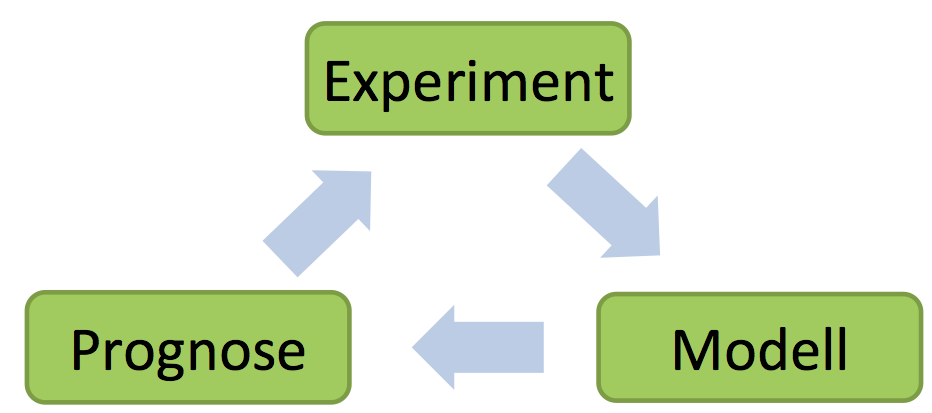
\includegraphics[width=7cm]{images/induktiveslernen}
	\end{center}
	\caption{Kreislauf des induktiven Lernens}
	\label{abb:indukt}
\end{figure}
\vspace{0.5cm}
Eine weitere Methode ist die Quantitative Struktur-Aktivit�tsanalyse (QSAR) \cite{qsar}, bei der die Wirkung eines Molek�ls durch die molekularen Eigenschaften beschrieben werden kann. Durch QSAR kann eine Prognose, wie ein Molek�l sich bei einer Interaktion verh�lt, aufgestellt werden.\\
Der Begriff der pharmakologisch motivierten molekularen �hnlichkeit \cite{chemoinformatik} erm�glicht die Vorhersage anhand bereits bekannter Verbindungen. Zwei Molek�le werden als �hnlich bezeichnet, wenn sie sich in biologischen Systemen �hnlich verhalten.\\
Besonders bei den letzten beiden vorgestellten Verfahren eignet sich der Einsatz von computergest�tzte Verfahren.
Computergest�tzte Verfahren oder Werkzeuge finden in der modernen Chemie immer mehr Anwendung. Sie eignen sich besonders, da mit ihrer Hilfe gro�e Mengen an Informationen analysiert werden k�nnen (z.B. durch QSAR). Die sogenannte Chemieinformatik ist ein Gebiet der Chemie, die mit Hilfe von Methoden der Informatik versucht chemische Probleme zu l�sen. \cite{textbook}\cite{chemoinformatik}\cite{introduction}

Die molekulare �hnlichkeit von zwei Molek�len kann durch Einsatz von computergest�tz-\\ten Methoden auf verschiedene Arten untersucht werden. Sie kann durch topologische Indizes (z.B. Randi\'{c}-Index \cite{randic}), durch Fingerprint Generierung \cite{chemoinformatik}\cite{introduction}, bei der angegeben wird welche strukturellen Eigenschaften oder funktionellen Gruppen ein Molek�l enth�lt, oder auch mit �hnlichkeits- bzw. Distanzma�en (z.B. Tanimoto-Koeffizient \cite{matrices}) bestimmt werden. \cite{matrices}

Durch die Bestimmung der molekularen �hnlichkeit lassen sich nicht nur f�r einzelne Molek�le Vorhersagen zu den Interaktionen treffen, sondern auch f�r Molek�lmengen, die sich mit chemischen Mustern \cite{Daylightsma}\cite{gci} beschreiben lassen. Die Interaktion einer Verbindung mit anderen erfolgt meist auf Grund von bestimmten Strukturen oder funktionellen Gruppen innerhalb der Verbindung. Diese zu untersuchenden Eigenschaften lassen sich mit chemischen Mustern ausdr�cken (z.B. ein Muster, welches alle Molek�le beschreibt, die eine Nitrogruppe enthalten). Diese Muster stellen eine Beschreibung einer Molek�lmenge, bestehend aus Molek�len mit den relevanten Eigenschaften, dar. Sie k�nnen dazu genutzt werden Molek�le zu filtern. So ist eine Aussortierung von beispielsweise Toxikophoren, oder auch das Ausw�hlen von Verbindungen mit gew�nschten Eigenschaften m�glich.

Um es in der Chemieinformatik zu erm�glichen Interaktionen vorherzusagen oder zu analysieren, k�nnen chemische Verbindungen in eine Graphenstruktur �berf�hrt werden, wodurch eine mathematische Analyse m�glich wird.\\
Es handelt sich bei solchen Molek�lgraphen \cite{introduction} um ungerichtete endliche markierte Graphen. Dabei werden die Atome als Knoten und die chemischen Bindungen als Kanten betrachtet. Die so entstehenden Graphen k�nnen anschlie�end im Rahmen der Graphentheorie auf gemeinsame Eigenschaften oder Teilstrukturen untersucht werden, um die molekulare �hnlichkeit zu bewerten. Analog erfolgt die �bertragung von chemischen Mustern in eine Graphenstruktur, welche dann f�r den Vergleich aus der graphentheoretischen Sicht genutzt werden kann. Dies ist n�tig, da auch chemische Muster und somit die beschriebenen Molek�lmengen �hnlichkeiten zueinander aufweisen k�nnen. Ein Vergleich w�rde es erm�glichen festzustellen, ob es eine Hierarchie der chemischen Muster gibt, ob es in einer Menge von chemischen Mustern redundante Muster gibt, aber auch um festzustellen, ob sich bestimmte Teilstrukturen oder funktionelle Gruppen in bereits genutzten Mustern wiederfinden. Bislang gibt es in die Chemieinformatik keine Methode um chemische Muster auf ihre �hnlichkeit zu �berpr�fen. In der Informatik und den, zu chemischen Mustern �quivalenten, regul�ren Ausdr�cken\footnote[1]{Zeichenkette, die eine Menge von Zeichenketten beschreibt} gibt es Ans�tze zur �hnlichkeitsanalyse. Meist basiert die Analyse auf der Generierung und Vergleich von endlichen Automaten\footnote[2]{Modell zur Beschreibung eines Verhaltens nach Eingabe einer Anfrage, bestehend aus einer endlichen Anzahl an Zust�nden, Zustands�berg�ngen und Aktionen \cite{endlauto}}\cite{regex}.
Die Komplexit�t der chemischen Muster verhindert eine �bertragung dieses Ansatzes auf das hier vorgestellte Problem, weshalb es n�tig ist ein neues Verfahren zu entwickeln. Ein naiver Ansatz w�re es die Molek�le, die von chemischen Mustern beschrieben werden zu vergleichen. Es kann passieren, dass verschiedene Muster durch Zufall die gleichen Molek�le beschreiben, indem z.B. zwei funktionelle Gruppen, jeweils als chemisches Muster beschrieben, gemeinsam und dennoch unabh�ngig in einem Molek�l auftreten. Bei diesem Ansatz muss es einen Abgleich geben, der �berpr�ft welche Atome in dem Molek�l von den Mustern beschrieben werden. Zudem erm�glicht dieser Vergleich von chemischen Mustern es nicht eine allgemeine Aussage �ber die �hnlichkeit zu treffen, da der Vergleich abh�ngig von der genutzten Molek�lmenge ist, die unter Umst�nden keine Molek�le beinhaltet, die von chemischen Mustern beschrieben werden.

Eine L�sung zum Vergleich zweier chemischer Muster wird in dieser Arbeit vorgestellt und beschrieben. Der L�sungsansatz wurde im Rahmen einer Masterarbeit von A. Mashychev \cite{Master} entwickelt und in der hier vorgestellten Arbeit weiterentwickelt und implementiert.

\subsection{Grundlagen}
F�r die in den folgenden Kapiteln beschriebene Arbeit ist es n�tig einige Begriffe und Grundlagen zu erkl�ren.
\subsubsection{SMILES} \label{sssec:smiles}
Unter einem SMILES (\textit{Simplified Molecular Input Line Entry Specification}) versteht man eine String-Repr�sentation von Molek�len. Entwickelt wurde diese Beschreibung mit Hilfe von ASCII-Zeichen und Bindungssymbolen. Der Vorteil von SMILES gegen�ber anderen Molek�lrepr�sentationen ist die Eigenschaft, dass die Molek�lbeschreibung in einer Zeile kompakt und effizient gespeichert werden kann.
Ein effizientes Arbeiten mit SMILES-Strings ist dadurch m�glich, dass ein SMILES-String leicht in einen Molek�lgraphen �berf�hrt werden kann. Die Grammatik eines SMILES-Strings gliedert sich in f�nf grundlegene Einheiten:
\begin{itemize}
	\item Atome (mit impliziten und expliziten Eigenschaften)
	\item Bindungen
	\item Verzweigungen
	\item Unterbrechungen
	\item Ringe
\end{itemize}
Kovalent gebundene Atome stehen benachbart in einer Zeichenkette. Bindungprimitive, die Beschreibungen von chemischen Bindungen, werden zwischen den jeweiligen Atomen angegeben. \cite{gci}\cite{smiles}

\subsubsection*{Atome} \label{sssec:smilesatome}
Die Atom-Beschreibung innerhalb eines SMILES-String erfolgt �ber die Angabe des Element-Symbols. Eine Besonderheit ist dabei die Angabe eines Atoms durch \texttt{*}. Das \texttt{*} gilt dabei als nicht spezifiziertes oder unbekanntes Atom, einer sogenannten \textit{Wildcard}. Des Weiteren werden Elementen, die im \textit{organic subset}\footnote[1]{Teilmenge der chemischen Elemente bestehend aus B, C, N, O, P, S, F, Cl, Br, I und *. Diese Elemente k�nnen ohne \texttt{[]} angegeben werden. Sie besitzen in dieser Form die implizite Anzahl an Bindungen zu Wasserstoffen aufgrund der kleinst m�glichen Valenz, keine Ladung, keine Chiralit�t und keine isotopischen Eigenschaften. \cite{Daylightsmi}} enthalten sind von den restlichen Elementen des Periodensystems unterschieden.\\
Eine weitere Besonderheit betrifft die Atome C, N, P, O, S, As, Se und *. Diese Atome k�nnen, durch Angabe der Element-Symbole als Kleinbuchstaben, als aromatische Atome interpretiert werden.

Neben den Element-Symbol, werden Atome mit Hilfe weiterer Eigenschaften, den sogenannten Atomprimitiven, beschrieben.
Grunds�tzlich gilt dabei folgender Syntax f�r die Angabe einer Atombeschreibung:
\begin{center}
	\texttt{[<mass>symbol<chiral><hcount><sign<charge>>]}
\end{center}

Tabelle \ref{tab:smilesatom} beschreibt die einzelnen Eigenschaften und wie sie in einem SMILES repr�sentiert werden. Beispiel \ref{bsp:smiles0} zeigt drei unterschiedliche SMILES und ihre zugeh�rigen Molek�le, die sie beschreiben. \cite{gci}\cite{Daylightsmi}\\

\begin{table}[h]
	\centering
	\captionabove{Beschreibung der m�glichen Atomprimitive. \texttt{Symbol} beschreibt, wie in Kapitel \ref{sssec:smilesatome} erl�uter das Element-Symbol. \texttt{@} gibt an, dass die folgenen Atome gegen den Uhrzeigersinn gelistet sind, bei \texttt{@@} sind sie im Uhrzeigersinn gelistet. \texttt{n} ist bei den Atomprimitiven eine nat�rliche Zahl. \cite{gci}}
	\begin{tabular}{| l | l | l |}
		\hline Atomprimitiv & SMILES-Syntax & Beschreibung\\
		\hline \texttt{<mass>} & \texttt{<n>} & Masse des Atoms \\
		\texttt{symbol} & \texttt{Symbol} & Element-Symbol nach Periodensystem \\
		\texttt{<chiral>} & \texttt{@@} oder \texttt{@} & Chiralit�t an tetraedrischen Kohlenstoffen \\ 
		\texttt{<hcount>} & \texttt{H<n>} & Anzahl gebundener Wasserstoff-Atome \\
		\texttt{<sign<charge>>} & \texttt{-<n>} oder \texttt{+<n>} & Ladung des Atoms \\ \hline
	\end{tabular}
	\label{tab:smilesatom}
\end{table}

\begin{bsp}
	\label{bsp:smiles0}
\end{bsp}
\begin{tabular}{m{0.22\textwidth} m{0.1\textwidth} m{0.1\textwidth}}
	\texttt{O} & beschreibt & H$_2$O \\
	&&\\
	\texttt{[Fe+2]} & beschreibt & Fe$^{+2}$\\
	&&\\
	\texttt{N[C@@](F)(C)C(=O)O} & beschreibt & 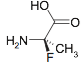
\includegraphics[width=2cm]{images/SMILESBspChir}
\end{tabular}

\subsubsection*{Bindungen}
Innerhalb eines SMILES-Strings wird zwischen den, in Tabelle \ref{tab:smilesbond} beschriebenen, Bindungen unterschieden. Beispiel \ref{bsp:smiles1} zeigt drei Beispiele von SMILES und die Molek�le, die sie repr�sentieren. \cite{smiles}\\

\begin{table}[h]
	\centering
	\captionabove{Beschreibung der m�glichen Bindungsprimitiven. \texttt{default} beschreibt den Fall, dass zwischen zwei Atombeschreibungen keine Bindung angegegben wird. \texttt{\char`\\} und \texttt{/} beschreiben eine Konfigurationsisomerie, die \textit{cis-trans-Isomerie}, die im Beispiel \ref{bsp:smiles1} dargestellt ist. \cite{Daylightsmi}}
	\begin{tabular}{| l | l |}
		\hline SMILES-Syntax & Beschreibung\\
		\hline \texttt{default} & Einfachbindung \\
		\texttt{-} & Einfachbindung \\
		\texttt{=} & Doppelbindung \\ 
		\texttt{\#} & Dreifachbindung \\
		\texttt{:} & aromatische Bindung (1.5 fach) \\ 
		\texttt{\char`\\ und /} & nach oben und nach unten Bindung als  Stereospezifikation \\
		& von Doppelbindungen (angegeben in Paaren) \\ \hline
	\end{tabular}
	\label{tab:smilesbond}
\end{table}

\begin{bsp}
	\label{bsp:smiles1}
\end{bsp}
\begin{tabular}{m{0.1\textwidth} m{0.1\textwidth} m{0.1\textwidth}}
	\texttt{C=O} & beschreibt & 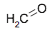
\includegraphics[width=1.2cm]{images/SMILESBsp1}\\
	\texttt{F/C=C/F} & beschreibt & 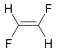
\includegraphics[width=1.5cm]{images/SMILESBsp5}\\
	\texttt{F/C=C\char`\\F} & beschreibt & 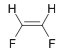
\includegraphics[width=1.5cm]{images/SMILESBsp4}
\end{tabular}
	
\subsubsection*{Verzweigungen}
Eine Verzweigung innerhalb des Molek�lgraphens wird durch \texttt{()} angegeben. Die Ausdr�cke k�nnen gereiht und geschachtelt werden. Beispiel \ref{bsp:smiles2} zeigt eine solche Verzweigung eines Molek�ls. In diesem Molek�l sind mindestens zwei Verzweigungen zur Beschreibung n�tig. \cite{gci}\cite{smiles}\\
\begin{bsp}
	\label{bsp:smiles2}
\end{bsp}
\begin{tabular}{m{0.13\textwidth} m{0.1\textwidth} m{0.1\textwidth}}
	\texttt{CC(C)C(=O)O} & beschreibt & 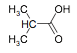
\includegraphics[width=1.9cm]{images/SMILESBsp2}
\end{tabular}

\subsubsection*{Unterbrechungen}
Um eine Unterbrechung zu kennzeichnen kann in der SMILES Sprache ein "`\texttt{.}"' genutzt werden, der zwischen zwei Atombeschreibungen steht. Dadurch werden Atome, die nicht miteinander verbunden sind kenntlich gemacht, wie Beispiel \ref{bsp:smilespunkt} zeigt. \cite{gci}\cite{Daylightsmi}\\
\begin{bsp}
	\label{bsp:smilespunkt}
\end{bsp}
\begin{tabular}{m{0.13\textwidth} m{0.1\textwidth} m{0.1\textwidth}}
	\texttt{[Na+].[Cl-]} & beschreibt & Na$^+$ Cl$^-$ \\
\end{tabular}

\subsubsection*{Ringe}
Eine Ringbindung kann durch die Angabe eines Zahlenpaares dargestellt werden. Dabei wird eine Bindung in einem Molek�l, die einen Ringschluss hervorrufen w�rde entfernt und an die beiden beteiligten Atome ein passendes Zahlenpaar angef�gt, wie das Beispiel \ref{bsp:smiles3} zeigt. \cite{Daylightsmi}\\
\begin{bsp}
	\label{bsp:smiles3}
\end{bsp}
\begin{tabular}{m{0.09\textwidth} m{0.1\textwidth} m{0.1\textwidth}}
	\texttt{C1CCCCC1} & beschreibt & 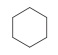
\includegraphics[width=1.5cm]{images/SMILESBsp3}
\end{tabular}

\newpage
\subsubsection{SMARTS} \label{sssec:smarts}
Die Abk�rzung SMARTS steht f�r \textit{SMiles ARbitrary Target Specification} und bezeichnet eine Sprache, die chemischer Muster und deren Eigenschaften mit Hilfe von kurzen Stringbeschreibungen repr�sentiert.
Die SMARTS Sprache ist eine Spezifizierung von SMILES. Daher gilt jeder SMILES ist auch ein valider SMARTS. SMARTS-Ausdr�cke besitzen zus�tzliche Atom- bzw. Bindungsprimitive, die im Folgenden erkl�rt werden. \cite{Daylightsma}\cite{gci}

\subsubsection*{Atome}
Die SMARTS Sprache besitzt eine m�chtigere Beschreibung im Vergleich zur SMILES-Sprache. Dazu wurden die Atomprimitive beschrieben in Kapitel \ref{sssec:smiles} um die, in Tabelle \ref{tab:smartsatomprimi} dargestellten, Atomprimitive erweitert. \cite{Daylightsma}\cite{gci}\\ 
\begin{table}[h]
	\centering
	\captionabove{Beschreibung der, f�r SMARTS hinzukommenden, Atomprimitive. \texttt{n} und \texttt{c} sind hierbei nat�rliche Zahlen. Die Zeile "`default-Wert"' gibt den Wert an den ein Atomprimitiv einnimmt, wenn \texttt{n} und \texttt{c} nicht angegeben sind. \cite{Daylightsma}}
	\begin{tabular}{| l | l | l |}
		\hline Syntax & Beschreibung & default-Wert \\
		\hline \texttt{a} & aromatisches Atom & - \\
		\texttt{A} & aliphatisches Atom & - \\ 
		\texttt{D<n>} & \textless n\textgreater Bindungen zu nicht-H Atomen & n = 1 \\
		\texttt{X<n>} & Atom mit insgesamt \textless n\textgreater Bindungen & n = 1 \\ 
		\texttt{x<n>} & Atom mit \textless n\textgreater Ringbindungen & n \textgreater = 1 \\ 
		\texttt{v<n>} & Atom mit Bindungsordnung \textless n\textgreater & n = 1 \\
		\texttt{H<n>} & Atom mit \textless n\textgreater Bindungen zu expliziten Wasserstoffen & n = 1\\
		\texttt{h<n>} & Atom mit \textless n\textgreater Bindungen zu impliziten Wasserstoffen & n \textgreater = 1 \\
		\texttt{R<n>} & in \textless n\textgreater Ringen eines SSSR & jedes Ringatom \\
		\texttt{r<n>} & in dem kleinsten Ring einer SSSR mit  \textless n\textgreater Atomen & jedes Ringatom \\
		\texttt{\#<n>} & Atom mit Ordnungszahl \textless n\textgreater & - \\
		\texttt{@<c><n>} & Chiralit�tsklasse \textless c\textgreater, Chiralit�t \textless n\textgreater & - \\
		\texttt{@<c><n>?} & Chiralit�tsklasse \textless c\textgreater, Chiralit�t \textless n\textgreater oder nicht spezifiziert & - \\ \hline
	\end{tabular}
	\label{tab:smartsatomprimi}
\end{table}

\subsubsection*{Bindungen}
Die Bindungsprimitiven der SMARTS Sprache werden um die in Tabelle \ref{tab:smartsbondprimi} dargestellten Eigenschaften erweitert.\\

\begin{table}[h]
	\centering
	\captionabove{Beschreibung der f�r SMARTS hinzukommenden Bindungsprimitiven. \texttt{default} beschreibt den Fall, dass zwischen zwei Atombeschreibungen keine Bindung angegegben wird. \cite{Daylightsma}\cite{gci}}
	\begin{tabular}{| l | l |}
		\hline SMARTS-Syntax & Beschreibung \\ 
		\hline \texttt{default} & Einfach- oder aromatische Bindung \\ 
		\texttt{?\char`\\ und ?/} & nach oben oder nicht spezifiziert \\
		& und nach unten oder nicht spezifiziert\\
		$\sim$ & beliebige Bindung (Wildcard) \\
		\texttt{@} & beliebige Bindung in einem Ring\\ \hline
	\end{tabular}
	\label{tab:smartsbondprimi}
\end{table}

\subsubsection*{Logische Operatoren}
Atom- und Bindungsprimitive k�nnen in der SMARTS Sprache mit Hilfe von logischen Operatoren verkn�pft werden. In der Tabelle \ref{tab:smartslogprimi} sind die Operatoren aufgelistet.\\
\begin{table}[h]
	\centering
	\captionabove{Beschreibung der logischen Operatoren in der SMATRTS Sprache, wobei es sich bei \texttt{SMARTSExp} um ein Atom- oder Bindungsprimitiv handelt. \cite{gci}}
	\begin{tabular}{| l | l |}
		\hline SMARTS-Syntax & Beschreibung \\
		\hline \texttt{!<SMARTSExp>} & nicht \texttt{!<SMARTSExp>} \\ 
		\texttt{<SMARTSExp1>\&<SMARTSExp2>} & \texttt{<SMARTSExp1>} und \texttt{<SMARTSExp2>} (starke Bindung)\\
		\texttt{<SMARTSExp1>,<SMARTSExp2>} & \texttt{<SMARTSExp1>} oder \texttt{<SMARTSExp2>} \\
		\texttt{<SMARTSExp>;<SMARTSExp>} & \texttt{<SMARTSExp1>} und \texttt{<SMARTSExp2>} (schwache Bindung)\\ \hline
	\end{tabular}
	\label{tab:smartslogprimi}
\end{table}

\subsubsection*{Unterbrechungen}
Auch in der SMARTS Sprache sind Atom-Unterbrechungen, also nicht miteinander verbundene Atome mit Hilfe eines "`\texttt{.}"' m�glich. Bei der SMARTS Sprache ist es zus�tzlich noch m�glich, durch Setzung von Klammern, ein unterschiedliches Betrachten von SMARTS-Ausdr�cken zu erm�glichen (siehe Tabelle \ref{tab:smartsunterbrprimi}).\\
\begin{table}[h]
	\centering
	\captionabove{Beschreibung f�r m�gliche Unterbrechungen innerhalb der SMATRTS Sprache. Bei \texttt{SMARTSExp} handelt es sich um ein Atomprimitiv. \cite{gci}}
	\begin{tabular}{| l | l |}
		\hline SMARTS-Syntax & Beschreibung \\ 
		\hline \texttt{<SMARTSExp1>.<SMARTSExp2>} & \texttt{<SMARTSExp1>} und \texttt{<SMARTSExp2>}\\ & k�nnen, m�ssen aber nicht verbunden sein\\
		\texttt{(<SMARTSExp1>).(<SMARTSExp2>)} & \texttt{<SMARTSExp1>} und \texttt{<SMARTSExp2>}\\ & treffen in verschiedenen (nicht kovalent\\ & verbundenen) Fragmenten\\
		\texttt{(<SMARTSExp1>).<SMARTSExp2>} & \texttt{<SMARTSExp1>} und \texttt{<SMARTSExp2>}\\ & treffen unabh�ngig voneinander\\ \hline
	\end{tabular}
	\label{tab:smartsunterbrprimi}
\end{table}

\subsubsection*{Rekursive Ausdr�cke}
Ein weiterer Zusatz der SMARTS Sprache ist die Erweiterung der Beschreibung von Atom\-eigenschaften, durch rekursive Ausdr�cke. Unter rekursiven Ausdr�cken versteht man die Beschreibung der Atomumgebung durch einen weiteren SMARTS-Ausdruck in der Form \texttt{\$(SMARTSExp)}. \cite{Daylightsma}\cite{gci}\\
\begin{bsp}
\end{bsp}
\label{bsp:smarts1}
\begin{tabular}{l l}
	\texttt{ [C[\$(CO)]} & beschreibt ein Kohlenstoffatom, welches als Umgebung kovalent an ein\\ & Sauerstoffatom gebunden ist
\end{tabular}

\newpage
\subsubsection{Subgraph-Isomorphie}
Ein weiterer Begriff, der vorab erl�utert werden muss, ist der der Subgraph-Isomorphie. Die Subgraph-Isomorphie ist ein $\mathcal{NP}$-vollst�ndiges Graphenproblem der theoretischen Informatik. \cite{introduction}\cite{gci}\cite{graph}\\
Gegeben sei ein Graph $G=(V,E)$. $V$ beschreibt die Menge an Knoten, die im Graphen $G$ enthalten sind und $E$ die Menge an Kanten des Graphens, so dass gilt:
\begin{align}
E \subseteq \{(v_i,v_j) | v_i,v_j \in V, v_i \neq v_j\}
\end{align}
Gegeben sei  ein weiterer Graph $G'=(V',E')$. 
Besitzen zwei Graphen $G$ und $G'$ die gleiche Menge an Knoten $V = V'$ und die gleiche Menge an Kanten $E = E'$ so gilt auch $G = G'$, sie sind also gleich oder automorph.
Gilt f�r $G'(V',E')$
\begin{align}
V' \subseteq V,E' \subseteq E \cap (V' \times V')
\end{align}
so ist $G'$ ein Subgraph von $G$. Gilt weiter
\begin{align}
	E' = \{ (v_i,v_j) \in E | v_i,v_j \in V' \},
\end{align}
so ist $G'$ ein induzierter Subgraph von $G$.

Gegeben seien nun zwei Graphen $G$ und $F$, die eine unterschiedliche Knotenmenge haben, also nicht gleich sein k�nnen. Sie lassen sich dennoch durch den Isomorphiebegriff miteinander vergleichen.
Die Isomorphie ist ein Fachbegriff der Graphentheorie und wird geschrieben als $G \simeq F$. Ein Graph $G$ ist zu einem anderen Graph $F$ genau dann isomorph, wenn eine bijektive Abbildung $m: V_F \to V_G$ existiert mit
\begin{align}
	(v_i,v_j) \in E_F \Leftrightarrow (m(v_i),m(v_j)) \in E_G.
\end{align}
Die Abbildung $m$ wird dann als Isomorphismus von $F$ nach $G$ bezeichnet.
Unter der Graphenisomorphie bezeichnet man einen Isomorphismus zweier Graphen gleicher Gr��e.
Besitzt Graph $F$ eine geringerer Anzahl an Knoten und Kanten als $G$, spricht man von Subgraph-Isomorphie, falls $F$ zu einem Teilgraphen von $G$ isomorph ist, also gilt
\begin{align}
	 V_F \to V_{G'},V_{G'} \subseteq V_G 
\end{align}
mit
\begin{align}
	(v_i,v_j) \in E_F \Leftrightarrow (m(v_i),m(v_j)) \in E_{G'}
\end{align}
f�r einen induzierten Subgraph, bzw.
\begin{align}
	(u,v) \in E_F \Rightarrow (m(u),m(v)) \in E_{G'}
\end{align}
%
% EOF
%
%
% L�sungsstrategie
%
\def\bigcircle{(0:0cm) ellipse (2.0cm and 1.0cm)}
\def\bigcircletwo{(0:0cm) ellipse (2.0cm and 1.0cm)}
\def\bigcirclemove{(0:-1cm) ellipse (2.0cm and 1.0cm)}
\def\bigcirclemovetwo{(0:1cm) ellipse (2.0cm and 1.0cm)}
\def\smallcircle{(0:0.4cm) ellipse (1.5cm and 0.5cm)}
\def\smallcircletwo{(0:-0.4cm) ellipse (1.5cm and 0.5cm)}
\def\AM{(0:0cm) ellipse (2.0cm and 1.0cm)}
\def\ZM{(0:5cm) ellipse (2.0cm and 1.0cm)}

\section{L�sungsstrategie}
In dieser Arbeit wird ein Verfahren vorgestellt, das es erm�glicht zwei chemische Muster auf eine Teilmengen-Relation zu untersuchen. Dabei wird zwischen Anfrage- und Zielmuster unterschieden. Wird eine Teilemengen-Relation festgestellt so erfolgt die Ausgabe der L�sung durch ein eindeutiges \textit{Mapping} des Anfrage- und Zielmusters. Dieses \textit{Mapping} ordnet den Atomen Anfragemusters das dazugeh�rigen Atom des Zielmusters zu.

Mit dieser L�sung kann herausgefunden werden, ob unterschiedlich definierte Muster dennoch Molek�lmengen beschreiben, die eine Teilmengen-Relation entsprechen. Somit k�nnen, wie im Kapitel \ref{sssec:einleitung} beschrieben, zum Beispiel bei einer Beschreibung der gleichen Molek�lmenge redundante Muster identifiziert werden.

Im folgenden Kapitel soll ein �berblick �ber die entwickelten Konzepte \cite{Master} und die Struktur der L�sung des in Kapitel \ref{sssec:einleitung} vorgestellten Problems gegeben werden.

\subsection{Konzepte} \label{ssec:konzepte}
Zum besseren Verst�ndnis werden im Folgenden die entwickelten Kontzepte des Verfahrens erl�utert, die eine Untersuchung auf Teilmengen-Relationen erm�glichen.

\subsubsection{Relationen} \label{sssec:rel}
Die vorliegende Arbeit behandelt den Vergleich von chemischen Mustern anhand von Teilmengen-Relationen. Das entwickelte Verfahren kann chemische Muster auf vier Teil-\\mengen-Relationen �berpr�fen. Gleichheit ($=$), Untermenge ($\subseteq$), Obermenge($\subseteq$) und Schnitt ($\cap$).
Die genaue Definition dieser Teilmengen-Relationen soll in diesem Abschnitt beschrieben werden, wobei zwischen Anfrage- ($A$) und Zielmuster ($Z$) unterschieden wird. Die Mengen an Molek�len, die vom Anfrage- bzw. Zielmuster beschrieben wird werden als $AM$ und $ZM$ bezeichnet und werden in diesem Kapitel zur Veranschaulichung als Venn-Diagramme pr�sentiert.\\
\begin{center}
	\begin{tikzpicture}
	\begin{scope}[fill opacity=0.3]
	\fill[green] \AM;
	\end{scope}
	\begin{scope}[fill opacity=0.3]
	\fill[cyan] \ZM;
	\end{scope}
	
	\draw \AM;
	\draw \ZM;
	
	\node[align=left] at (0,0) {$AM$};
	\node[text=black] at (5,0) {$ZM$};
	\end{tikzpicture}
\end{center}
\subsubsection*{Gleichheit}
Wenn zwei Beschreibungen von chemische Muster in allen atomaren und strukturellen Eigenschaften �bereinstimmen, dass hei�t die beschriebenen Molek�lmengen verhalten sich wie im folgenden dargestellten Venn-Diagramm,\\
\begin{center}
\begin{tikzpicture}
\begin{scope}[fill opacity=0.3]
\fill[green] \bigcircle;
\end{scope}
\begin{scope}[fill opacity=0.3]
\fill[cyan] \bigcircletwo;
\end{scope}

\draw \bigcircle;
\draw \bigcircletwo;

\node[text=black] at (0,0) {$AM$ und $ZM$};
\end{tikzpicture}
\end{center}
dann gilt:\\
\begin{align}
	A = Z
\end{align}

\subsubsection*{Untermenge}
Wenn das Anfragemuster in seinen atomaren und strukturellen Eigenschaften im Vergleich zum Zielmuster spezifizierter oder gleich weit spezifiziert ist, sich die Molek�lmengen der beiden chemischen Muster wie folgt verhalten,\\

\begin{figure}[h]
    \begin{center}
	\begin{minipage}{4.5cm}
		\begin{center}
			\begin{tikzpicture}
			\begin{scope}[fill opacity=0.3]
			\fill[green] \smallcircletwo;
			\end{scope}
			\begin{scope}[fill opacity=0.3]
			\fill[cyan] \bigcircle;
			\end{scope}
			
			\draw \smallcircletwo;
			\draw \bigcircle;
			
			\node[align=left] at (-0.4, 0) {$AM$};
			\node[text=black] at (1.5, 0) {$ZM$};
			\end{tikzpicture}
		\end{center}
	\end{minipage}
	\begin{minipage}{1cm}
		\centering
		bzw.
	\end{minipage}
	\begin{minipage}{4.5cm}
		\begin{center}
			\begin{tikzpicture}
			\begin{scope}[fill opacity=0.3]
			\fill[green] \bigcircle;
			\end{scope}
			\begin{scope}[fill opacity=0.3]
			\fill[cyan] \bigcircletwo;
			\end{scope}
			
			\draw \bigcircle;
			\draw \bigcircletwo;
			
			\node[text=black] at (0,0) {$AM$ und $ZM$};
			\end{tikzpicture}
		\end{center}
	\end{minipage}
	\end{center}
\end{figure}

dann gilt:
\begin{align}
	A \subseteq Z
\end{align}

\subsubsection*{Obermenge}
Wenn das Anfragemuster in seinen atomaren und strukturellen Eigenschaften im Vergleich zum Zielmuster allgemeiner oder gleich weit spezifiziert ist, sich die Molek�lmengen der beiden chemischen Muster also wie folgt verhalten,\\

\begin{figure}[h]
	\begin{center}
		\begin{minipage}{4.5cm}
			\begin{center}
				\begin{tikzpicture}
				\begin{scope}[fill opacity=0.3]
				\fill[green] \bigcircle;
				\end{scope}
				\begin{scope}[fill opacity=0.3]
				\fill[cyan] \smallcircle;
				\end{scope}
				
				\draw \bigcircle;
				\draw \smallcircle;
				
				\node[text=black] at (-1.5, 0) {$AM$};
				\node[align=left] at ( 0.4, 0) {$ZM$};
				\end{tikzpicture}
			\end{center}
		\end{minipage}
		\begin{minipage}{1cm}
			\centering
			bzw.
		\end{minipage}
		\begin{minipage}{4.5cm}
			\begin{center}
				\begin{tikzpicture}
				\begin{scope}[fill opacity=0.3]
				\fill[green] \bigcircle;
				\end{scope}
				\begin{scope}[fill opacity=0.3]
				\fill[cyan] \bigcircletwo;
				\end{scope}
				
				\draw \bigcircle;
				\draw \bigcircletwo;
				
				\node[text=black] at (0,0) {$AM$ und $ZM$};
				\end{tikzpicture}
			\end{center}
		\end{minipage}
	\end{center}
\end{figure}

dann gilt:
\begin{align}
	A \supseteq Z
\end{align}

\subsubsection*{Schnitt}
Zwei chemische Muster haben in zwei F�llen einen gemeinsamen, nicht leeren Schnitt.
Entweder wenn sie durch logische Alternative einen �berlappung von atomaren oder strukturellen Eigenschaften besitzen, oder es innerhalb des Anfragemusters Teilstrukturen gibt, die eine Untermenge des Zielmusters beschreiben sowie Teilstrukturen, die eine Obermenge des Zielmusters beschreiben. Verhalten sich also die beiden chemischen Muster in ihrer Molek�lmenge wie folgt,\\

\begin{center}
\begin{tikzpicture}
\begin{scope}[fill opacity=0.3]
\fill[green] \bigcirclemove;
\end{scope}
\begin{scope}[fill opacity=0.3]
\fill[cyan] \bigcirclemovetwo;
\end{scope}

\draw \bigcirclemove;
\draw \bigcirclemovetwo;

\node[text=black] at (-1.5, 0) {$AZ$};
\node[align=left] at (1.5, 0) {$ZM$};
\end{tikzpicture}
\end{center}

dann gilt:
\begin{align}
	A \cap Z
\end{align}

\subsubsection{Valenzzust�nde} \label{sssec:valenz}
Um zwei chemische Muster auf, die in Kapitel \ref{sssec:rel} vorgestellten, Teilmengen-Relationen zu �berpr�fen, muss es erm�glicht werden die Menge an Eigenschaften, die Atome und Bindungen beschreiben miteinander vergleichen zu k�nnen. F�r die komplexen Atombeschreibungen muss daf�r der Begriff des Valenzzustandes eingef�hrt werden. Allgemein versteht man unter einem Valenzzustand einen relevanten Zustand den ein zu untersuchendes Element einnehmen kann.
Durch den anschlie�enden Vergleich der chemisch m�glichen Valenzzust�nde von zwei zu untersuchenden Atomenbeschreibungen ist dann eine Untersuchung auf Teilmengen-Relationen m�glich.

In der hier vorgestellten L�sung besteht die Menge der Eigenschaften, die ein Valenzzustand eines Atoms beschreiben kann aus:
\begin{itemize}
	\item Atomname
	\item Atomnummer
	\item Atomgewicht
	\item Atomvalenz
	\item Anzahl der Einfachbindungen
	\item Anzahl der Doppelbindungen
	\item Anzahl der Dreifachbindungen
	\item Formalladung
	\item Anzahl der Bindungen zu Wasserstoffatomen
	\item ob das Atom aromatisch ist
	\item in wie vielen Ringen eines SSSR\footnote[1]{\textit{smallest set of smallest rings}} sich das Atom
	\item welche Gr��e hat der kleinsten SSSR-Ring in dem sich das Atom befindet
	\item Anzahl der Bindungen in Ringen
\end{itemize}
Anhand dieser Eigenschaften ist es m�glich die komplexe Struktur der Atombeschreibungen eines chemischen Musters zu kategorisieren und zu analysieren.

\subsubsection{Fingerprint} \label{sssec:fprint}
Anhand der Menge von chemisch m�glichen Valenzzust�nden eines in chemischem Mustern vorkommenden Atoms, kann ein Fingerprint generiert werden. Ein Fingerprint ist eine Repr�sentation aller, durch die oben beschriebenen Eigenschaften m�glichen Valenzzust�nde. Dieser Fingerprint in Form eines Bit-Arrays (siehe Abb. \ref{abb:bitarrayatom}) gibt an, ob eine Atombeschreibung ein Valenzzustand beschreibt (Bit auf "`1"' gesetzt) oder nicht (Bit auf "`0"' gesetzt).

\begin{figure}[h]
	\centering
	\begin{tikzpicture}
	\node[draw,fill=cyan!20,minimum height=1cm,minimum width = 1cm,xshift=1cm,font=\ttfamily][label={[xshift=1cm, yshift=1.2cm,rotate=50]\footnotesize erster Valenzzustand}](N1){1};
	\draw node[below=0cm of N1]{\scriptsize 0};
	\node[draw,fill=cyan!20,minimum height=1cm,minimum width = 1cm,xshift=2cm,font=\ttfamily][label={[xshift=1.1cm, yshift=1.3cm,rotate=50]\footnotesize zweiter Valenzzustand}](N2){1};
	\draw node[below=0cm of N2]{\scriptsize 1}; 
	\node[draw,fill=green!20,minimum height=1cm,minimum width = 1cm,xshift=3cm,font=\ttfamily][label={[xshift=1.1cm, yshift=1.2cm,rotate=50]\footnotesize dritter Valenzzustand}](N3){0};
	\draw node[below=0cm of N3]{\scriptsize 2}; 
	\node[draw,fill=cyan!20,minimum height=1cm,minimum width = 1cm,xshift=4cm,font=\ttfamily][label={[xshift=1.2cm, yshift=1.2cm,rotate=50]\footnotesize vierter Valenzzustand}](N4){1};
	\draw node[below=0cm of N4]{\scriptsize 3}; 
	
	\node [tape, draw,minimum size=1cm,tape bend top=none,
	tape bend height=0.4cm,rotate=90] at (4.8,0) (t) {};
	\node [tape, draw,minimum size=1cm,tape bend top=none,
	tape bend height=0.4cm,rotate=270] at (6.8,0) (t) {};
	
	\node at (5.8,0.5) {\dots};
	\node at (5.8,-0.5) {\dots};
	
	\node[draw,fill=green!20,minimum height=1cm,minimum width = 1cm,xshift=7.6cm][label={[xshift=1.2cm, yshift=1.4cm,rotate=50]\footnotesize vorletzter Valenzzustand}](N5){0} ;
	\node[draw,fill=green!20,minimum height=1cm,minimum width = 1cm,xshift=8.6cm][label={[xshift=1.1cm, yshift=1.3cm,rotate=50]\footnotesize letzter Valenzzustand}](N6){0} ;
	\draw node[below=0cm of N5]{\scriptsize 164206}; 
	\draw node[below=0cm of N6]{\scriptsize 164207}; 
	\end{tikzpicture}
	\caption{Schematische Darstellung eines Fingerprints f�r eine Atombeschreibung}
	\label{abb:bitarrayatom}
\end{figure}

Der Fingerprint f�r den Vergleich zwischen zwei Bindungen kann ohne den Begriff der Valenzzust�nde erstellt werden. Ben�tigt wird ein Bit-Array bestehend aus f�nf Bits, die die folgenden Bindungen beschreiben:
\begin{itemize}
	\item[1. Bit:] Einfachbindung
	\item[2. Bit:] Doppelbindung
	\item[3. Bit:] Dreifachbindung
	\item[4. Bit:] Ringbindung
	\item[5. Bit:] Aromatische Bindung
\end{itemize}

\begin{figure}[h]
	\centering
	\begin{tikzpicture}
	\node[draw,fill=cyan!20,minimum height=1cm,minimum width = 1cm,xshift=1cm,font=\ttfamily][label={[xshift=0.9cm, yshift=0.9cm,rotate=50]\footnotesize Einfachbindung}](N1){1};
	\draw node[below=0cm of N1]{\scriptsize 0};
	\node[draw,fill=cyan!20,minimum height=1cm,minimum width = 1cm,xshift=2cm,font=\ttfamily][label={[xshift=0.8cm, yshift=0.9cm,rotate=50]\footnotesize Doppelbindung}](N2){1};
	\draw node[below=0cm of N2]{\scriptsize 1}; 
	\node[draw,fill=green!20,minimum height=1cm,minimum width = 1cm,xshift=3cm,font=\ttfamily][label={[xshift=0.9cm, yshift=1cm,rotate=50]\footnotesize Dreifachbindung}](N3){0};
	\draw node[below=0cm of N3]{\scriptsize 2}; 
	\node[draw,fill=cyan!20,minimum height=1cm,minimum width = 1cm,xshift=4cm,font=\ttfamily][label={[xshift=0.8cm, yshift=0.8cm,rotate=50]\footnotesize Ringbindung}](N4){1};
	\draw node[below=0cm of N4]{\scriptsize 3}; 
	\node[draw,fill=green!20,minimum height=1cm,minimum width = 1cm,xshift=5cm,font=\ttfamily][label={[xshift=0.8cm, yshift=0.9cm,rotate=50]\footnotesize arom. Bindung}](N5){0};
	\draw node[below=0cm of N5]{\scriptsize 4};  
	\end{tikzpicture}
	\caption{Schematische Darstellung eines Fingerprints f�r eine Bindungsbeschreibung}
	\label{abb:bitarraybond}
\end{figure}

Abbildung \ref{abb:bitarraybond} zeigt schematisch, wie dieses Bit-Array f�r den Fingerprint einer Bindung aufgebaut ist. Hier wird beispielsweise eine Bindung, die sowohl eine Einfach-, Doppel- oder Ringbindung beschreibt dargestellt.

\newpage
\subsection{Struktur} \label{ssec:struktur}
Anhand der in Kapitel \ref{ssec:konzepte} erl�uterten Konzepte ist es m�glich das Verfahren zur Untersuchung auf Teilmengen-Relationen zu realisieren.
Es gliedert sich in sechs grundlegende Schritte.
Ein groben �berblick �ber die Struktur wird im Folgenden anhand der Abbildung \ref{abb:workflow} gegeben. Die Schritte sind in Kapitel \ref*{realisierung} detailiert beschrieben. 
 
Die Eingaben des Verfahrens beinhalten ein Anfragemuster mit Atomen (durch "`VA"' mit eindeutiger Identifikationsnummer in der Abbildung \ref{abb:workflow} beschrieben) sowie Bindungen (durch "`EA"' und eindeutiger Nummer beschrieben). Das Anfrage-Muster hat eine beliebige Gr��e (Ausgegrauter Bereich ab Atom "`VA2"'). Das Zielmuster hat die Atome- ("`VZ"') und Bindungsbezeichnung ("`EZ"') und hat ebenfalls eine beliebige Gr��e. Zu den beiden Mustern wird noch eine der vier m�glichen Teilmengen-Relation angegeben.

Im ersten Schritt werden die Muster aufbereitet und gefiltert. Die Aufbereitung erfolgt durch die eindeutige Kennzeichnung jedes Atoms (Knoten) der Muster durch ein . Anschlie�end wird je nach Teilmengen-Relation �berpr�ft, ob ein Vergleich der gegebenen Muster m�glich ist (siehe Abbildung \ref{abb:workflow} Schritt 1).

Der zweite Schritt wird ausgef�hrt, falls die �berpr�fung der Muster positiv war. Ansonsten erfolgt keine Ausgabe, da keine bijektive Abbildung gefunden wurde. In ihm werden f�r alle Atome und Bindungen der Muster Fingerprints erstellt.

Im dritten Schritt werden anhand der gegebenen Teilmengen-Relation die Fingerprints verglichen. Die Fingerprints der Knoten des Anfragemusters werden mit allen Fingerprints der Knoten des Zielmusters paarweise verglichen (in Abbildung \ref{abb:workflow} entsprechen die gr�nen Pfeile einer positiven �berpr�fung einer Teilmengen-Relation, rote Pfeile einer negativen �berpr�fung).

Entsprechen zwei Fingerprints der gegebenen Teilmengen-Relation, so wird im vierten Schritt in der Relations-Matrix der entsprechende Eintrag auf "`1"' gesetzt.

Im f�nften Schritt werden die gewonnenen Matrizen an einen Algorithmus zur Untersuchung auf Subgraph-Isomorphie �bergeben.

Das Ergebnis des gefundenen Isomorphismus wird dann in Form eines eindeutigen \textit{Mappings} als Ausgabe im letzten Schritt gebracht und ausgegeben.

\begin{figure}[h]
	\begin{center}
	\includegraphics[width=17cm]{images/Workflow}
	\end{center}
	\caption{Schematischer Ablauf des entwickelten Verfahrens.}
	\label{abb:workflow}
\end{figure}

%
% EOF
%
%
% Realisierung
%
\section{Realisierung} \label{realisierung}
Das Programm \textit{SmartsSmarts} wurde, wie in Kapitel \ref{ssec:struktur} beschrieben, in sechs Schritten realisiert. Im folgenden Kapitel sollen diese Schritte erl�utert werden.

Grundlage des Programms zum Vergleich von chemischen Mustern sind die in Kapitel \ref{sssec:smarts} vorgestellten SMARTS-Ausdr�cke.
Dem Programm werden neben einem Anfrage-SMARTS und Ziel-SMARTS zudem die zu untersuchende Teilmengen-Relation �bergeben.

\subsection{Genutze Software}
Das in dieser Arbeit vorgestellte Verfahren wurde im Rahmen der NAOMI-Softwartebibliothek \cite{naomi} des Zentrums f�r Bioinformatik (ZBH) der Universit�t Hamburg implementiert. Aus den folgende Modulen wurden Funktionen und Klassen genutzt:
\begin{enumerate}
	\setlength\itemsep{0em}\setlength\parskip{0em}
	\item \texttt{Chemistry}
	\item \texttt{SmartsParser}
	\item \texttt{Molecule}
	\item \texttt{SmartsMatcher}
\end{enumerate}
An welchen Stellen das \textit{SmartsSmarts}-Programm die Module nutzt wird in Abbildung \ref{fig:softwarestruk} (Kapitel \ref{sec:softwarearch}) gezeigt.

\subsection{Aufarbeitung und Auswahl}\label{ssec:vorverarbeitung}
Der Anfrage- und Ziel-SMARTS wird zun�chst in eine Form gebracht, die es erm�glicht im letzten Schritt des Verfahrens das \textit{Mapping} zu erzeugen. Die dazu genutzten \textit{Label} sind eindeutige Identifikationsnummern, die als \texttt{:ID} an die Knoten eines SMARTS-Ausdrucks gef�gt werden k�nnen. Dabei wird jedes Label einmalig an das Vergleichspaar aus Anfrage- und Ziel-SMARTS vergeben. Bestehende \textit{Label} werden �bernommen.\\
Anschlie�end werden f�r Anfrage- und Ziel-SMARTS �berpr�ft, ob ein Vergleich grund-\\s�tzlich anhand der Knoten-Anzahl und der gegebenen Relation m�glich ist (siehe Tabelle \ref{tab:anzahlcheck}). F�r die Schnitt-Relation ($\cap$) ist zu beachten, dass Anfrage- und Ziel-SMARTS die gleiche Anzahl an Knoten haben m�ssen, damit ein nicht leerer Schnitt vorliegt. Grund daf�r ist, dass die Schnitt-Menge zweier SMARTS-Muster ein SMARTS-Ausdruck beschreiben, welcher eine Untermenge von Anfrage- und Ziel-SMARTS sein soll. W�ren die beiden Muster unterschiedlich gro�, w�re der nicht leere Schnitt maximal so gro� wie der kleinere SMARTS-Ausdruck. F�r das gr��ere Muster kann also keine Untermengen-Relation vorliegen.\\

\begin{table}[h]
	\centering
	\captionabove{Anzahl�berpr�fung der Knoten des Anfrage-SMARTS ($Query$) und Ziel-SMARTS ($Target$)}
	\begin{tabular}{| c | l |}
		\hline Relation & Bedingung \\
		\hline $=$ and $\cap$ & $QueryNodeCount = TargetNodeCount$ \\
		$\subseteq$ & $QueryNodeCount >= TargetNodeCount$ \\
		$\supseteq$ & $QueryNodeCount <= TargetNodeCount$ \\
		\hline
	\end{tabular}
	\label{tab:anzahlcheck}
\end{table}

\subsection{Fingerprintgenerierung}
Die Basis f�r die Untersuchung auf eine bestimmte Teilmengen-Relation wird in diesem Schritt gewonnen. Anhand der Fingerprints von Knoten und Kanten k�nnen zwei chemische Muster miteinander verglichen werden.
In Kapitel \ref{sssec:valenz} und \ref{sssec:fprint} wurde bereits das Konzept des Fingerprints beschrieben.
Beide SMARTS-Ausdr�cke werden in eine digitale Graphenstruktur �bertragen. �ber diesen Graphen wird anschlie�end iteriert um f�r jeden Knoten und jede Kante den Fingerprint zu erstellen.\\
F�r Knoten werden, wie Tabelle \ref{tab:smartvalenz} zeigt, Eigenschaften ausgelesen und anhand dieser der Fingerprint generiert.\\

\begin{table}[h]
	\centering
	\captionabove{Eigenschaften der Valenzzust�nde f�r Atome und ihre zugeh�rigen SMARTS-Atomprimitive}
	\begin{tabular}{| l | l |}
		\hline Eigenschaft & abgeleitet aus SMARTS-Atomprimitiv \\
		\hline Element & \texttt{*}, \texttt{a}, \texttt{A} und alle Elementnamen \\
		Atomnummer & \texttt{\#n} \\
		Atomvalenz & \texttt{v<n>} \\
		Anzahl der Einfachbindungen & \texttt{D<n>}, \texttt{H<n>} \\
		Anzahl der Doppelbindungen & \texttt{D<n>} \\
		Anzahl der Dreifachbindungen & \texttt{D<n>} \\
		Formalladung & \texttt{+<n>}, \texttt{-<n>} \\
		Anzahl zu Wasserstoffatomen & \texttt{D<n>}, \texttt{H<n>} \\
		ob das Atom aromatisch ist & \texttt{*}, \texttt{a}, \texttt{A} und alle Atomnamen \\
		in wie vielen Ringen eines SSSR & \texttt{R<n>} \\
		sich das Atom befindet  & \\
		welche Gr��e hat der kleinsten SSSR- & \texttt{r<n>} \\
		Ring in dem sich das Atom befindet & \\
		Anzahl der Bindungen in Ringen & \texttt{x<n>} \\
		\hline
	\end{tabular}
	\label{tab:smartvalenz}
\end{table}
Die Generierung erfolgt durch eine sequentielle Abfrage und Abgleich aller Eigenschaften und dementsprechender Bit-Setzung. Ausgegangen wird von einem Bit-Array bei dem jedes Bit auf "`0"' gesetzt ist. Im ersten Schritt werden, wie im Algorithmus \ref{alg:fingerprint1} beschrieben, die Bits der Valenzzust�nde, die nicht durch die Atomnamen-Eigenschaften des Knotens beschrieben sind, auf "`1"' gesetzt. Zudem wird in diesem Schritt bereits die Aromazit�t untersucht, die im sp�teren Verlauf genutzt wird.

Die Eigenschaft der Atommasse (\texttt{<n>}) kann anhand des Fingerprints nicht verglichen werden, da die Menge an m�glichen Atommassen nicht im Umfang der Valenzzust�nde enthalten ist. Diese Eigenschaft zwischen zwei zu vergleichenden Knoten wird vor der Fingerprintgenerierung abgeglichen. Die Trennstellen-Eigenschaft der SMARTS-Sprache ist in dem hier entwickelte Konzept nicht ber�cksichtigt.

\begin{algorithm}[H]
\caption{Fingerprintgenerierung Ausschnitt 1 \cite{Master}} \label{alg:fingerprint1}
\begin{algorithmic}[1]
\Procedure{TakePropertyFingerprint}{$node$}

\State $node\_is\_aliphatic =$ \texttt{true}
\State $node\_is\_aromatic =$ \texttt{true}
\ForAll{$\big(i \in [1,nof\_valenceStates]\big)$}
	\State $sec\_temp\_bit\_array[i] =$ \texttt{true}
\EndFor
\ForAll{$\big(node\_Symbol = \Call{GetNodesSymbol}{node}\big)$} \Comment Abbildung Atomname
		
	\ForAll{$\big(i \in [1,nof\_valenceStates]\big)$}
		\State $temp\_bit\_array[i] =$ \texttt{false}
	\EndFor
	
	\NoThen	
	\If{$\big(node\_symbol \ne SMARTS\_ANY\_ATOM\big)$}
		\ForAll{$\big(i \in [1,nof\_valenceStates]\big)$}
			\If{$\big(node\_symbol = \Call{GetSymbol}{valencestates[i]}\big)$}
				\State $temp\_bit\_array[i] =$ \texttt{true}
			\EndIf
			\NoThen
		\EndFor

	\NoThen
		
	\If{$\big(\Call{NodeSymbolNegationFlag}{node} == \texttt{true}\big)$}
		\ForAll{$\big(i \in [1,nof\_valenceStates]\big)$}
			\If{\big($temp\_bit\_array[i] ==$ \texttt{true}$\big)$}
				\State $temp\_bit\_array[i] = $\texttt{false}
			\Else
				\State $temp\_bit\_array[i] = $\texttt{true}
			\EndIf
			\NoThen
		\EndFor
    \EndIf
	\Else
	    \ForAll{$\big(i \in [1,nof\_valenceStates]\big)$}
	    \State $temp\_bit\_array[i] =$ \texttt{true}
	    \EndFor

		\If{$\big(\Call{NodeSymbolNegationFlag}{node} == \texttt{true}\big)$}
			\If{$\big(\Call{NodeIsAliphatic}{node} == \Call{NodeIsAromatic}{node}\big)$}
				\ForAll{$\big(i \in [1,nof\_valenceStates]\big)$}
					\State $temp\_bit\_array[i] =$ \texttt{false}
				\EndFor
			\EndIf
		\EndIf
	\EndIf
	\NoThen
	\If{$\big(\Call{NodeIsAliphatic}{node} != \texttt{true}\big)$}
		\State $node\_is\_aliphatic =$ \texttt{false}
	\EndIf
	\NoThen
	\If{$\big(\Call{NodeIsAromatic}{node} != \texttt{true}\big)$}
		\State $node\_is\_aliphatic =$ \texttt{false}
	\EndIf
	\State $sec\_temp\_bit\_array = temp\_bit\_array \land sec\_temp\_bit\_array$
\EndFor
\State $bit\_array = bit\_array \lor sec\_temp\_bit\_array$
\EndProcedure
\end{algorithmic}
\end{algorithm}

Die meisten Eigenschaften k�nnen anschlie�end durch einen Abgleich von Graphen-Eigen\-schaften und Valenzzust�nden im Bit Array weiter gepr�ft werden und gegebenenfalls weitere Bits auf "0" gesetzt werden.
Im Algorithmus \ref{alg:fingerprint2} und Algorithmus \ref{alg:fingerprint3} sind die Verarbeitung der Eigenschaften der Bindungen (\texttt{D<n>}) und der Aromazit�t beschrieben, da diese nicht direkt aus der Graphenstruktur abzulesen sind.

\begin{algorithm}[H]
\caption{Fingerprintgenerierung Ausschnitt 2 \cite{Master}} \label{alg:fingerprint2}
\begin{algorithmic}[1]
	\ForAll{$\big(i \in [1,nof\_valenceStates]\big)$}
		\State $temp\_bit\_array[i] =$ \texttt{false}
	\EndFor
	
	\ForAll{$\big(node\_degree = \Call{GetNodesDegree}{node}\big)$} \Comment Abbildung \texttt{D<n>}
		\ForAll{$\big(i \in [1,nof\_valenceStates]\big)$}
			\NoThen
			\If {$ \begin{pmatrix*}[l]
					&\Big(node\_degree \ne \big(\Call{GetNofBonds}{valencestates[i]}\\
					
					&-\Call{GetNofHydrogens}{valencestates[i]}\big) \textbf{ and}\\
					
					&\big(\Call{NodeDegreeNegationFlag}{node} == \texttt{false}\big)\Big)\\
					
					\textbf{or} & \Big(node\_degree = \big(\Call{GetNofBonds}{valencestates[i]}\\ 
					
					&-\Call{GetNofHydrogens}{valencestates[i]}\big) \textbf{ and}\\
					
					& (\Call{NodeDegreeNegationFlag}{node} == \texttt{true})\Big)\\
					
					\textbf{and} & bit\_array[i] == \texttt{true}
				\end{pmatrix*} $}
					\State $bit\_array[i] =$ \texttt{false}
			\EndIf
		\EndFor
		\State $temp\_bit\_array = temp\_bit\_array \lor bit\_array$
	\EndFor
	\State $bit\_array = bit\_array \land temp\_bit\_array$
\end{algorithmic}
\end{algorithm}
\begin{algorithm}[H]
	\caption{Fingerprintgenerierung Ausschnitt 3 \cite{Master}} \label{alg:fingerprint3}
	\begin{algorithmic}[1]
		\ForAll{$\big(i \in [1,nof\_valenceStates]\big)$} \Comment{Abbildung Aromazit�t}
		\NoThen
		\If {$ \begin{pmatrix*}[l]
			& \big(node\_is\_aromatic == \texttt{true} \textbf{ and } node\_is\_aliphatic == \texttt{false}\\
			
		  	& \textbf{and } \Call{IsAromatic}{valencestates[i]} == \texttt{false}\big)\\
		  	
		  	\textbf{or} & \big(node\_is\_aromatic == \texttt{false} \textbf{ and } node\_is\_aliphatic == \texttt{true}\\
		  	
		  	& \textbf{and } \Call{IsAromatic}{valencestates[i]} == \texttt{true}\big)\\
			
			\textbf{and} & bit\_array[i] == \texttt{true} 
			\end{pmatrix*}$}
		\State $bit\_array[i] =$ \texttt{false}
		\EndIf
		\EndFor
	\end{algorithmic}
\end{algorithm}
F�r die Kanten k�nnen die Eigenschaften zur Fingerprintgenerierung direkt aus der Graphenstruktur abgelesen werden. Tabelle \ref{tab:smartsbind} stellt dabei die Eigenschaften, die der Fingerprint enth�lt, in Zusammenhang mit den darstellenden SMARTS-Bindungsprimitiven.\\

\begin{table}[h]
	\centering
	\captionabove{F�r die Fingerprintgenerierung genutzte Eigenschaften einer Bindung und dazugeh�rige Bindungsprimitive}
	\begin{tabular}{| l | l |}
		\hline Eigenschaft & SMARTS-Bindungsprimitive \\ 
		\hline Einfachbindung & \texttt{-}, \texttt{/}, \texttt{\char`\\}, $\sim$\\
		Doppelbindung & \texttt{=}, $\sim$\\
		Dreifachbindung & \texttt{\#}, $\sim$\\
		Ringbindung & \texttt{@}, $\sim$\\
		aromatische Bindung & \texttt{:}, $\sim$ \\ \hline
	\end{tabular}
	\label{tab:smartsbind}
\end{table}

Nicht alle Eigenschaften eines SMARTS-Ausdruck k�nnen in dem hier vorgestellten Verfahren verarbeitet werden. Zum Beispiel k�nnen die in Kapitel \ref{sssec:smarts} beschriebenen Rekursionen, die f�r SMARTS-Ausdr�cke genutzt werden, um Umgebungen von SMARTS-Primitiven zu definieren nicht beachtet werden. F�r weitere nicht unterst�tzte SMARTS-Primitve siehe Kapitel \ref{ssec:probleme}. L�sungsans�tze werden in Kapitel \ref{sec:ausblick} beschrieben.

\subsection{Vergleich und Aufbau Relation-Matrix} \label{ssec:relmatr}
F�r die Untersuchung auf einen Subgraphisomorphismus von zwei chemischen Mustern ben�tigt man Initial-Matrizen f�r Knoten und Kanten, die die m�glichen bijektiven Abbildungen der einzelnen Elemente repr�sentieren.
Anschlie�end wird die Initial-Matrix der Knoten und die der Kanten zusammen mit den Adjazenzmatrizen\footnote[1]{Matrix zugeh�rig zu einen Graphen, die durch "`1"' angeben, dass eine Kante zwischen zwei Knoten besteht oder durch "`0"', dass es keine Kante zwischen zwei Knoten gibt. Dabei besitzt sie f�r jeden Knoten eine Zeile ($i$) und eine Spalte ($j$). Ein Element ($i,j$) gibt die Adjazenz vom $i$-ten und $j$-ten Knoten an. \cite{graph}} der beiden chemischen Mustern an einen Algorithmus zur Berechnung des Isomorphismus �bergeben. In dieser Arbeit wurde dazu der Algorithmus nach Ullmann \cite{ullmann} verwendet.\\
Anhand der Fingerprints, die f�r alle Bestandteile der beiden zu untersuchenden SMARTS-Ausdr�cke erstellt wurden, k�nnen R�ckschl�sse auf die Teilmengen-Relationen gezogen werden.\\
F�r den Vergleich werden Bit-Operationen genutzt. Die Tabelle \ref{tab:bitop} zeigt welche Bit-Operationen dazu ausgef�hrt werden m�ssen, um die Teilmengen-Relationen zu �berpr�fen. Anschlie�end k�nnen mit den Ergebnissen der Vergleiche die Initial-Matrizen initialisiert werden. In diesem Kontext werden sie als Relations-Matrizen bezeichnet, da sie R�ckschl�sse auf Teilmengen-Relationen geben.\\

\begin{table}[h]
	\centering
	\captionabove{Ergibt die durchgef�hrte Bit-Operation aus der linken Spalte ein Bit-Array, welches keine auf "1" gesetzten Bits enth�lt, so gilt die in der rechten Spalte angegebene Teilmengen-Relation \cite{Master}}
	\begin{tabular}{| l | l |}
		\hline Bit-Operation & Teilmengen-Relation \\
		\hline $QueryArray \oplus TargetArray$ & $Query=Target$ \\
		$(QueryArray \land TargetArray)\oplus QueryArray$ & $Query\subseteq Target$ \\
		$(TargetArray \land QueryArray)\oplus TargetArray$ & $Query\supseteq Target$ \\ \hline
	\end{tabular}
	\label{tab:bitop}
\end{table}

Wird f�r zwei Knoten oder zwei Kanten festgestellt, dass die angegebene Teilmengen-Relation besteht so wird der Matrix Eintrag auf "`1"' gesetzt. Abbildung \ref{abb:matrix} zeigt ein Beispiel einer initialisierten Relations-Matrix von zwei SMARTS-Ausdr�cken.

\begin{figure}[h]
	\centering
	\begin{align*}
		\begin{pmatrix}
			0 & 1 & 1 & 1 \\
			1 & 0 & 0 & 0 \\
			1 & 1 & 1 & 1 \\
		\end{pmatrix}
	\end{align*}
	\caption{Die Matrix ist ein Beispiel einer Relations-Matrix der Teilmengen-Relation $\subseteq$, die mit dem Anfrage-SMARTS \texttt{P(=S)(S)S} und dem Ziel-SMARTS \texttt{S=P$\sim$[*,\#1]} initialisiert wurde. Die Spalten entsprechen den Knoten des Anfrage-SMARTS und die Zeilen den Knoten des Ziel-SMARTS}
	\label{abb:matrix}
\end{figure}

Zur �berpr�fung der Teilmengen-Relation $Query\cap Target$ kann keine einfache Bit-Opera-\\tion durchgef�hrt werden. Durch Zuhilfenahme der in Tabelle \ref{tab:bitop} beschriebenen Bit-Operationen k�nnen zwei Elemente auf $Query\cap Target$ gepr�ft werden. Zwei chemische Muster haben einen wie in Kapitel \ref{sssec:rel} nicht leeren Schnitt in zwei F�llen:

Sei $G^Q(V^Q,E^Q)$ die Graphenrepr�sentation des Anfrage-SMARTS und $G^T(V^T,E^T)$ die Graphenrepr�sentation des Ziel-SMARTS. Weiter sei ein Knoten $v \in V$ bestehend aus der Menge an logischen Alternativen $LA_v$, sowie eine Kante $e \in E$ bestehend aus der Menge an logischen Alternativen $LA_e$. F�r ein m�gliches \textit{Mapping} $M_{QT}$ bestehend aus Knoten-Paaren $(v_Q, v_T)$ und den impliziten Kanten-Paaren $(e_Q, e_T)$ muss gelten:
\begin{align}
\begin{split}
	& \Big[\forall (v_Q,v_T) \in M_{QT}:\Big(LA_{v_Q}=,\cap,\subset,\supset LA_{v_T}\Big)\\
	& \land \forall (e_Q,e_T) \in M_{QT}:\Big(LA_{e_Q}=,\cap,\subset,\supset LA_{e_T}\Big)\Big]\\	
	\land & \Big[\exists (v'_Q,v'_T) \in M_{QT}:\Big(LA_{v'_Q} \neq LA_{v'_T} \land LA_{v'_Q} \not\subset LA_{v'_T} \land LA_{v'_Q} \not\supset LA_{v'_T}\Big)\\
	& \lor \exists (e'_Q,e'_T) \in M_{QT}:\Big(LA_{e'_Q} \neq LA_{e'_T} \land LA_{e'_Q} \not\subset LA_{e'_T} \land LA_{e'_Q} \not\supset LA_{e'_T}\Big)\Big]
	\label{eq:fall1} 
\end{split}
\end{align} 

%\begin{align}
%\begin{split}
%& \Big[ \exists v_Q \in V^Q \exists v_T \in V^T :\Big( \exists a_Q \in LA_{v_Q} \exists a_T \in LA_{v_T} :\big( a_Q =,\subseteq,\supseteq a_T \big)\\	
%& \land  \exists a'_Q \in LA_{v^Q} \neq a_Q \exists a'_T \in LA_{v^T} \neq a_T :\big( a_Q' \neq a_T' \big) \Big)\\	
%& \land \forall v_Q' \in V^Q \forall v_T' \in V^T :\Big(  v'_Q \neq v_Q \land v'_T \neq v_T \land v_Q' =, \subseteq, %\supseteq v_T' \Big)\Big]\\	
%\lor & \Big[ \exists e_Q \in E^Q \exists e_T \in E^T :\Big( \exists a_Q \in LA_{e_Q} \exists a_T \in LA_{e_T} :\big( a_Q =,\subseteq,\supseteq a_T \big)\\	
%& \land  \exists a'_Q \in LA_{e^Q} \neq a_Q \exists a'_T \in LA_{e^T} \neq a_T : \big( a_Q' \neq a_T' \big) \Big)\\	
%& \land \forall e_Q' \in E^Q \forall e_T' \in E^T :\Big(  e'_Q \neq e_Q \land e'_T \neq e_T \land e_Q' =, \subseteq, \supseteq e_T' \Big)\Big]
%\label{eq:fall1alt} 
%\end{split}
%\end{align} 
oder
\begin{align}
\begin{split}
& \Big(\forall (v_Q,v_T) \in M_{QT}: \big(LA_{v_Q} =,\cap,\subset,\supset LA_{v_T}\big)\\
&\land \forall (e_Q,e_T) \in M_{QT}: \big(LA_{e_Q} =,\cap,\subset,\supset LA_{e_T}\big)\Big)\\
\land &\Big[\Big( \exists (v'_Q,v'_T),(v''_Q,v''_T) \in M_{QT}\backslash \{(v_Q,v_T)\}:\\
& \big((v'_Q,v'_T)\neq(v''_Q,v''_T) \land LA_{v'_Q} \subset LA_{v'_T} \land LA_{v''_Q} \supset LA_{v''_T} \big) \Big)\\
&\lor \Big( \exists (e'_Q,e'_T),(e''_Q,e''_T) \in M_{QT}\backslash \{(e_Q,e_T)\}:\\
& \big((e'_Q,e'_T)\neq(e''_Q,e''_T) \land LA_{e'_Q} \subset LA_{e'_T} \land LA_{e''_Q} \supset LA_{e''_T} \big) \Big)\Big]
\end{split}
\label{eq:fall2} 
\end{align}
%\begin{align}
%\begin{split}
%	&\Big( \big( \exists v_Q \in V^Q \exists v_T \in V^T ( v^Q \subset v^T ) \land \exists v'_Q \in V^Q \exists v'_T \in V^T (v'_Q \neq v_Q \land v'_T \neq v_T \land v'^Q \supset v'^T) \big)\\
%	& \lor \big( \exists e_Q \in E^Q \exists e_T \in E^T ( e^Q \subset e^T ) \land \exists e'_Q \in E^Q \exists e'_T \in E^T (e'_Q \neq e_Q \land e'_T \neq e_T \land e'^Q \supset e'^T) \big) \Big)\\
%	\land & \forall v''_Q \in V^Q \forall v''_T \in V^T \big( v''_Q \neq v'_Q \neq v_Q \land v''_T \neq v'_T \neq v_T \land v''^Q =,\subseteq,\supseteq v''^T \big) \\
%	\land & \forall e''_Q \in E^Q \forall e''_T \in E^T \big( e''_Q \neq e'_Q \neq e_Q \land e''_T \neq e'_T \neq e_T \land e''^Q =,\subseteq,\supseteq e''^T \big) \\
%	\end{split}
%	\label{eq:fall2alt} 
%\end{align}
Beispiel \ref{bsp:intersecone} zeigt, zwei SMARTS-Ausdr�cke f�r die Formel \eqref{eq:fall1} gilt. Ein Knoten erf�llt die Eigenschaft des zweiten Teils der Formel. Die restlichen Knoten erf�llen den ersten Teil.\\

\begin{bsp}
	\label{bsp:intersecone}
\end{bsp}
\begin{table}[h]
	\centering
	\begin{tabular}{l | c c c}
		Anfrage-SMARTS & \texttt{[Cl,I]} & $\sim$ & \texttt{O} \\
		Teilmengen-Relation & $\cap$ & $=$ & $=$ \\
		Ziel-SMARTS & \texttt{[Cl,F] }& $\sim$ & \texttt{O}\\
	\end{tabular}
\end{table}

Beispiel \ref{bsp:intersectwo} zeigt zwei SMARTS-Ausdr�cke bei denen Formel \eqref{eq:fall2} gilt. F�r mindestens einen Knoten gilt $\supset$, in diesem Beispiel ist es jeweils der letzte Knoten. Des Weiteren gilt f�r mindestens ein Knoten- oder Bindungspaar $\subset$, in diesem Beispiel die jeweils ersten beiden Knoten und die Bindung.\\

\begin{bsp}
\label{bsp:intersectwo}
\end{bsp}
\begin{table}[h]
	\centering
	\begin{tabular}{l | c c c}
		Anfrage-SMARTS & \texttt{[C;!R]} & $\sim$ & \texttt{O} \\
		Teilmengen-Relation & $\subset$ & $=$ & $\supset$ \\
		Ziel-SMARTS & \texttt{[\#6] }& $\sim$ & \texttt{[OH]}\\
	\end{tabular}
\end{table}

\subsection{Subgraphisomorphie Analyse}
Anhand der Relations-Matrizen von Knoten und Kanten ist es nun m�glich zwei Muster auf eine Subgraphisomorphismus zu untersuchen.

Mit der f�r die Knoten erzeugten Relations-Matrix, den jeweiligen Adjazenz-Matrizen und der Information zur Vereinbarkeit der Kanten durch die entsprechende Relations-Matrix wird durch den Algorithmus nach Ullmann ein Isomorphismus gesucht und die gefundenen bijektiven Abbildungen in Form von Permutationsmatrizen ausgegeben.

Bei der �berpr�fung auf eine Schnitt-Relation werden die Permutationsmatrizen in einem weiteren Schritt erneut auf diese Teilmengen-Relation gepr�ft. In diesem Schritt wird f�r die resultierende bijektive Abbildung gepr�ft, ob Formel \eqref{eq:fall1} oder Formel \eqref{eq:fall2} gelten.

\subsection{Kennzeichnung}
Zur eindeutigen Zuordnung der gefundenen Isomorphismen wurde anschlie�end eine �n-\\derung der \textit{Label} des Ziel-SMARTS erzeugt, die als Abbildung des Anfrage-SMARTS dienen. Durch diese Kennzeichnung der Knoten eines Anfrage-SMARTS in einem Ziel-SMARTS wird bei der Ausgabe deutlich welche Knoten eine Abbildung darstellen. Beispiel \ref{bsp:labelmapping} zeigt f�r die vier m�glichen Teilmengen-Relationen die Ausgabe der gefundenen \textit{Mappings}. Abbildung \ref{abb:solution} zeigt eine Visualisierung (erzeugt mit SMARTSviewer \cite{smartsview}\cite{smartsviewsoftware}) der Ergebnisse.\\

\begin{bsp}
	\label{bsp:labelmapping}
\end{bsp}
\begin{table}[h]
	\begin{tabular}{l l | l}
		\textbf{Gleichheit:} & Anfrage-SMARTS & \texttt{[C:1](=[O:2])[Cl,Br,I,F:3]}\\
		& Ziel-SMARTS & \texttt{[O:2]=[C:1]-[F,Cl,Br,I:3]}\\
		&&\\
		\textbf{Schnitt:} & Anfrage-SMARTS & \texttt{[\#7:1]-[N:2]=[O:3]}\\
		& Ziel-SMARTS & \texttt{[!\#7:3]$\sim$[NX2:2]$\sim$[NX1:1]}\\
		&&\\
		\textbf{Untermenge:} & Anfrage-SMARTS & \texttt{[O:1]=[C:2][N:3]=[N+:4]=[N-:5]}\\
		& Ziel-SMARTS & \texttt{[N:3]=[N+:4]=[N-:5]}\\
		&&\\
		\textbf{Obermenge:} & Anfrage-SMARTS & \texttt{[S:1][C:2]\#[N:3]}\\
		& Ziel-SMARTS & \texttt{[S:1](=[O:5])(=[O:6])[C:2]\#[N:3]}\\
	\end{tabular}
\end{table}

\begin{figure}[h!]
	\centering
	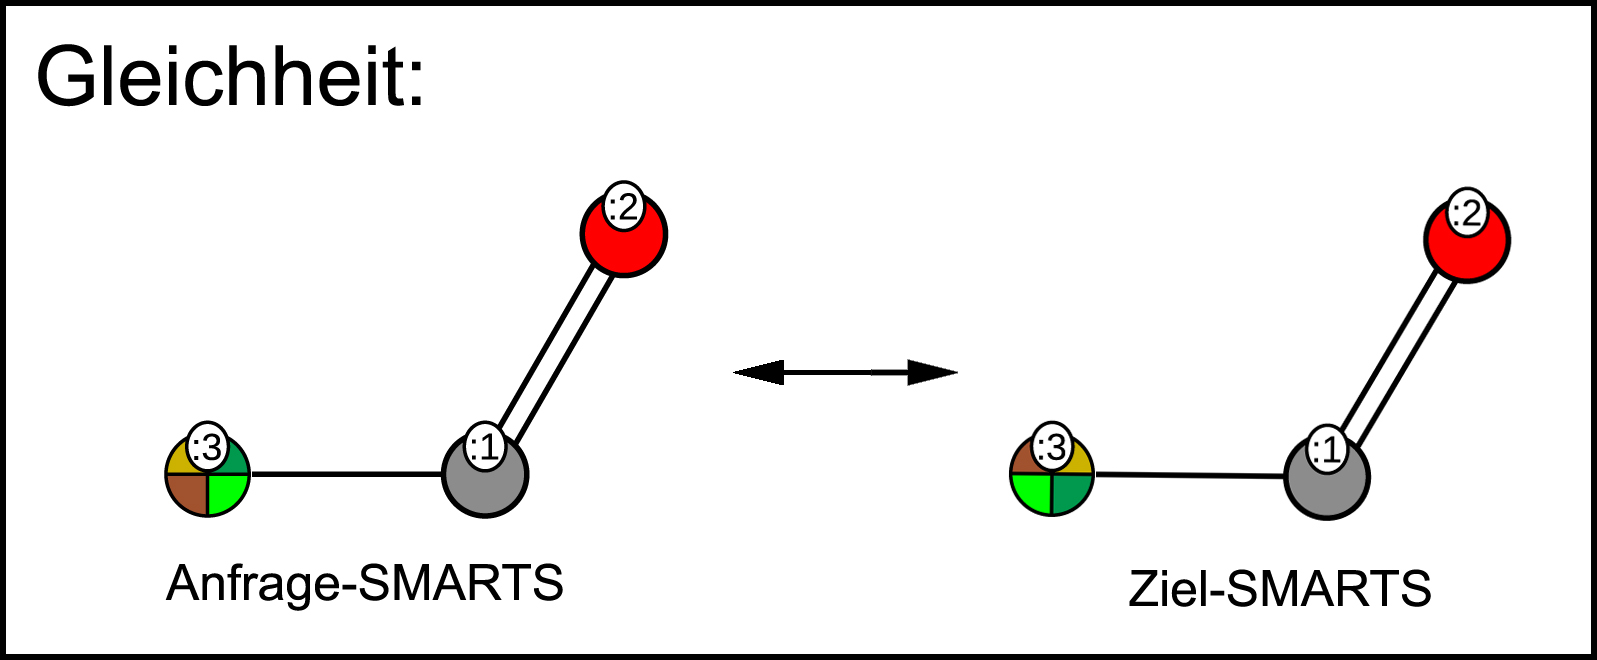
\includegraphics[width=10cm]{images/gleichmapping}\\
	\vspace{0.3cm}
	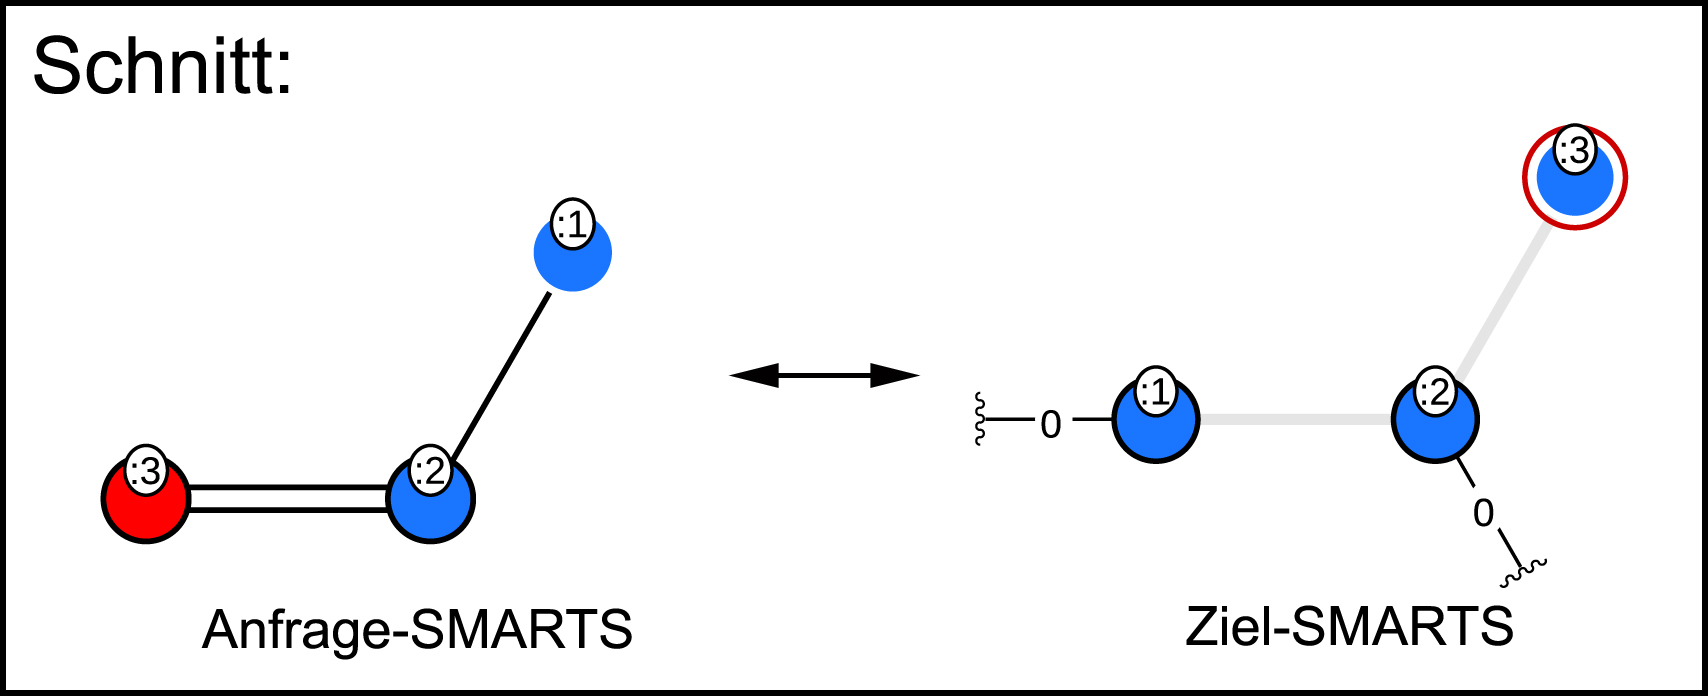
\includegraphics[width=11cm]{images/schnittmapping}\\
	\vspace{0.3cm}
	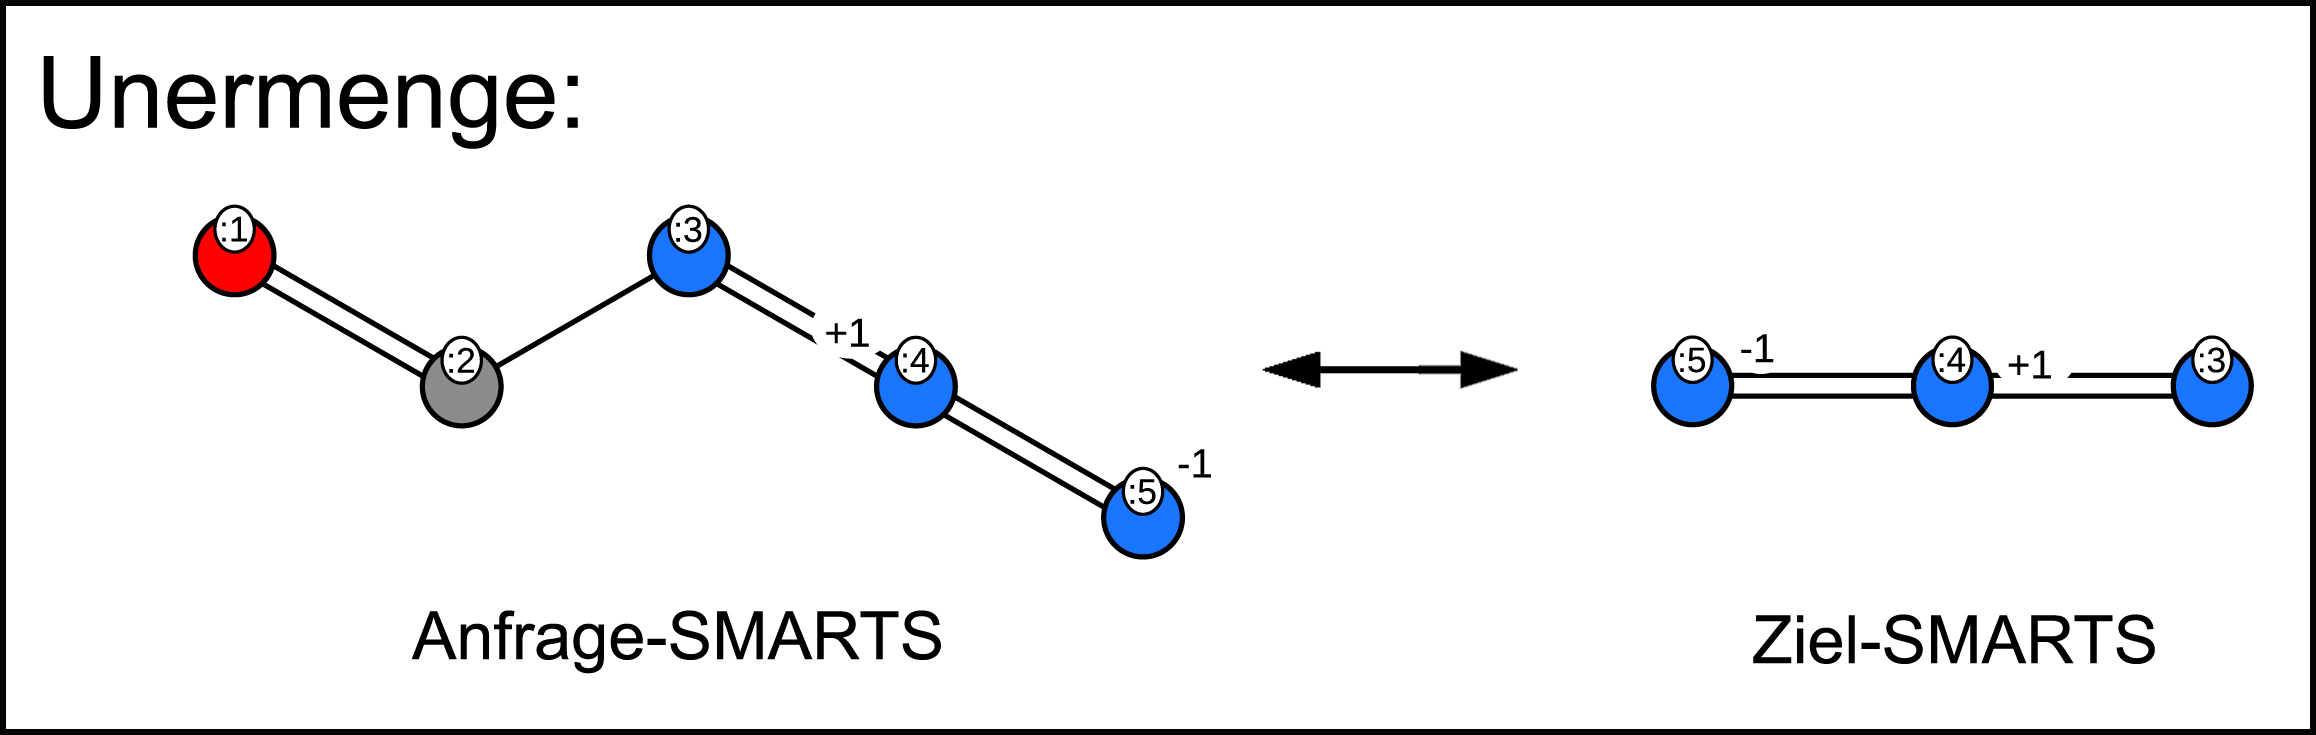
\includegraphics[width=12cm]{images/untermapping}\\
	\vspace{0.3cm}
	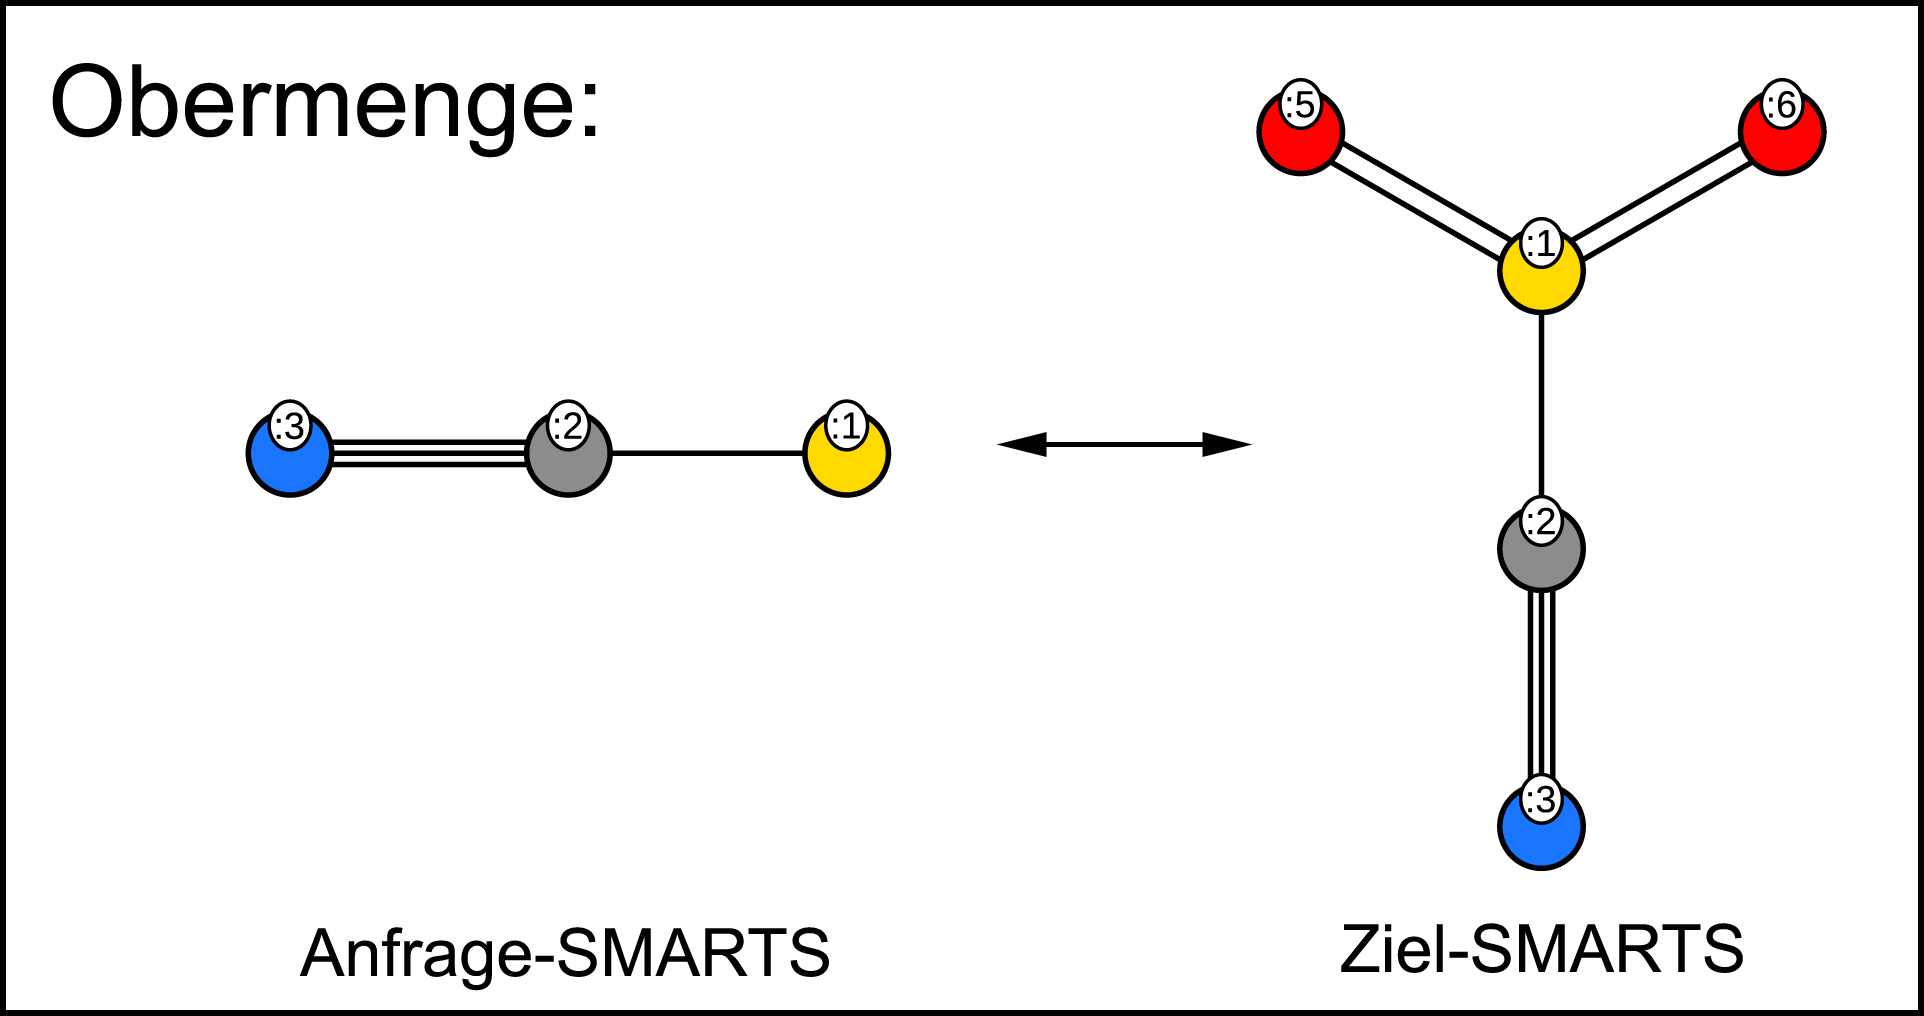
\includegraphics[width=10cm]{images/obermapping}
	\caption{Visualisierung der gefundenen \textit{Mappings} aus Beispiel \ref{bsp:labelmapping}.}
	\label{abb:solution}
\end{figure}
%
% EOF
%
\section{Evaluation}
\subsection{Testen}\label{ssec:test}
Zur �berpr�fung der Korrektheit des implementierten Verfahrens \textit{SmartsSmarts} wurden im ersten Schritt der Evaluation die Hauptfunktionen, die das Verfahren nutzt, auf korrekte Ergebnisse �berpr�ft. Welche Testfunktionen genutzt wurden wird in diesem Kapitel beschrieben.

\begin{description}
\item[\texttt{fingerprint:}]\hfill \\
Die Testfunktion pr�ft, ob bei der �bergaben von einem Knoten eines SMARTS-Ausdrucks ein Fingerprint generiert wurde, der die richtigen Bits gesetzt hat.

\item[\texttt{mapping:}]\hfill \\
�berpr�ft die Korrektheit der Funktion bei der anhand von zwei Fingerprints und einer Teilmengen-Relation ermittelt wird, ob die gew�nschte Teilmengen-Relation gefunden wurde.

\item[\texttt{nodeRelationMatrix:}]\hfill \\
Initialisiert eine Relations-Matrix und �berpr�ft, ob diese korrekt erstellt wurde.

\item[\texttt{smartsSmartsUllmann:}]\hfill \\
Testfunktion die ermittelt, ob bei der �bergabe von zwei SMARTS-Ausdr�cken und einer Teilmengen-Relation das erwartete \textit{Mapping} in Form einer Permutationsmatrix ausgegeben wird.

\end{description}

Durch die Testfunktionen konnten Fehler in der Finerprintgenerierung und der Isomorphismusanalyse durch den Algorithmus nach Ullmann identifiziert und behoben werden.

\subsection{Validierung}\label{ssec:validierung}
Nachdem die Korrektheit der einzelnen Funktionen getestet wurde, erfolgte anschlie�ende eine Validierung des implementierten Verfahrens.

Die Validierung erfolgt dabei �ber den Vergleich von Molek�lmengen. Es wurden 6~000 Molek�le aus der ZINC-Datenbank \cite{zinc} genutzt (siehe Anhang \ref{ssec:zinc}).\\
Die genutzten SMARTS-Ausdr�cke \cite{smartsdata} wurden vom Zentrum f�r Bioinformatik ver�ffentlicht. Der Datensatz beinhaltet 1~469 SMARTS-Ausdr�cke (siehe Anhang \ref{ssec:aasmarts}).

\subsubsection{Durchf�hrung}
Das implementierte Verfahren wurde validiert indem die Molek�lmengen der SMARTS-Ausdr�cken verglichen wurden.
Das Vorgehen gliedert sich dabei in zwei Schritte.\\
Im ersten Schritt wird f�r zwei SMARTS-Ausdr�cke und einer Teilmengen-Relation �ber-\\pr�ft, ob ein \textit{Mapping} gefunden wurde.\\
Schritt zwei �berpr�ft das Verhalten von Anfrage- und Ziel-SMARTS im Bezug auf das Treffen (\textit{Matching}) von Molek�len. Wenn ein \textit{Mapping} gefunden wird, wird �ber die Molek�lliste iteriert und gepr�ft ob Anfrage- und Ziel-SMARTS ihrer Teilmengen-Relation entsprechend das gleiche Molek�l treffen. Tabelle \ref{tab:validierung} zeigt welche Bedingungen f�r welche Teilmengen-Relation erf�llt sein muss.\\

\begin{table}[h]
	\centering
	\captionabove{�bersicht der Bedinungen, die die SMARTS-Ausdr�cke eines \textit{Mappings} erf�llen m�ssen, um f�r eine Teilmengen-Relation als valides \textit{Mapping} zu gelten. Betrachtet werden dabei die Teilmengen-Relationen Gleichheit, Untermenge und Obermenge.}
	\begin{tabular}{| c | l |}
		\hline Teilmengen-Relation & Bedingung des \textit{Matchings}\\
		\hline Gleichheit ($=$) & Anfrage-SMARTS und Ziel-SMARTS\\
		& m�ssen gleiches Molek�l treffen\\
		Untermenge ($\subseteq$) &   Wenn Anfrage-SMARTS Molek�l trifft,\\
		& muss auch Ziel-SMARTS treffen\\
		Obermenge ($\supseteq$) &   Wenn Ziel-SMARTS Molek�l trifft,\\
		& muss auch Anfrage-SMARTS treffen\\ \hline
	\end{tabular}
	\label{tab:validierung}
\end{table}

Falls kein \textit{Mapping} gefunden wird, wird ebenfalls �ber die Molek�lliste iteriert und f�r jedes Molek�l gepr�ft, ob beide SMARTS-Ausdr�cken das zu �berpr�fende Molek�l treffen. Ist dies der Fall werden die beiden SMARTS-Ausdr�cke zusammen mit der Teilmengen-Relation ausgegeben, um manuell ausschlie�en zu k�nnen, dass ein \textit{Mapping} nicht gefunden wurde. Solch ein Fall tritt auf, wenn innerhalb eines Molek�ls unterschiedliche Atome durch den SMARTS-Ausdruck beschrieben werden.

Die Schnitt-Relation kann mit dieser Methode nicht validiert werden, da nicht gew�hrleistet ist, dass der Teil des Schnittes des gefundenen \textit{Mappings} ein Molek�l trifft. Bei Beispiel \ref{bsp:validschnitt} und Abbildung \ref{abb:thyroxin} tritt der Fall ein, dass anhand der Molek�lmenge eine Validierung nicht m�glich ist. Beispiel \ref{bsp:validschnitt} zeigt ein \textit{Mapping} der Schnitt-Relation, wird nun das \textit{Matching}-Verhalten der beiden SMARTS-Ausdr�cke in Bezug auf das Molek�l aus Abbildung \ref{abb:thyroxin} verglichen, wird festgestellt, dass trotz eines gefundenen \textit{Mappings} die Molek�lmenge nicht vergleichbar ist.\\

\begin{bsp}
	\label{bsp:validschnitt}
\end{bsp}
\begin{table}[h]
	\centering
	\begin{tabular}{l l | l}
		\textbf{Schnitt-\textit{Mapping}:} & Anfrage-SMARTS & \texttt{[Cl,I:1]}$\sim$\texttt{[c:2]}\\
		& Ziel-SMARTS & \texttt{[Cl,F:1]}$\sim$\texttt{[c:2]}\\
	\end{tabular}
\end{table}

\begin{figure}[h]
	\centering
	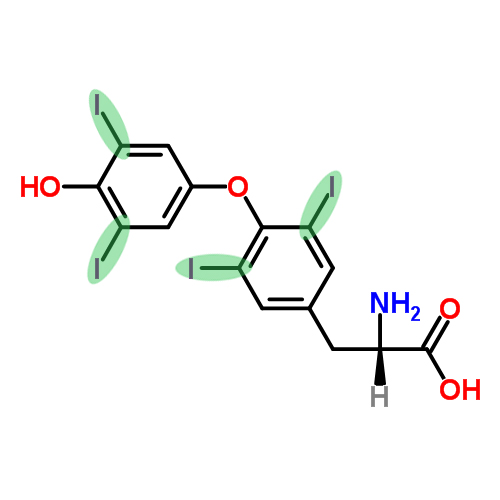
\includegraphics[width=5cm]{images/thyroxin}
	\caption{Levothyroxin mit gr�n gekenntzeichneten Teilstrukturen, bei denen der Anfrage-SMARTS das Molek�l trifft \cite{thyroxin}}
	\label{abb:thyroxin}
\end{figure}

\newpage
\subsubsection{Resultate}
Durch die Validierung konnte ein Fehler aufgedeckt werden, bei dem das Anh�ngen der \textit{Label} im Vorverarbeitungsschritt (siehe Kapitel \ref{ssec:vorverarbeitung}) fehlschlug. Dieser Fehler hat die Ausf�hrung des Verfahrens verhindert. Dieser wurde bei den Tests (siehe Kapitel \ref{ssec:test}) nicht aufgedeckt, da er nur bei einer Kombination aus aromatischen Elementnamen (z.B. \texttt{c}) mit Elementnamen bestehend aus zwei Zeichen (z.B. \texttt{Br}) auftritt.\\
Ein weiteres Fehlverhalten betrifft den zweiten Fall bei dem eine Schnitt-Relation festgestellt werden kann (siehe Kapitel \ref{ssec:relmatr} Gleichung \eqref{eq:fall2}). Dieser Fall wurde durch die Validierung kenntlich gemacht.

Nachdem die beschriebenen Probleme gel�st wurden, war es m�glich die Validierung erfolgreich durchzuf�hren. Bei einem Beispiel des Validierungsverfahrens wurde als Anfrage-SMARTS \texttt{N$\sim$[\#6]} zusammen mit der Angabe, dass alle vier Teilmengen-Relationen an das Programm \textit{SmartsSmarts} �bergeben. Als Ziel-SMARTS wurden die SMARTS-Ausdr�cke als Liste �bergeben. 431 SMARTS-Ausdr�cke konnten von dem Programm nicht verarbeiten werden (siehe Kapitel \ref{ssec:probleme}).
Es wurden 4 Untermengen-\textit{Mappings} und 109 Obermengen-\textit{Mappings} gefunden, welche alle durch die Validierung best�tigt werden konnten. Die F�lle, bei denen ohne \textit{Mapping} dennoch beide SMARTS-Ausdr�cke ein Molek�l getroffen wurden, wurden wie beschrieben manuell �berpr�ft. Es konnte kein fehlendes \textit{Mapping} festgestellt werden.\\
Neben diesem Beispiel wurde die Validierung mehrfach mit unterschiedlichen Anfrage-SMARTS erfolgreich durchgef�hrt.

\newpage
\subsection{Laufzeitanalyse}
F�r die Laufzeitanalyse wurde die ben�tigte Zeit des Verfahrens in Zusammenhang mit der Gr��e der genutzten SMARTS-Ausdr�cke gebracht. Durchgef�hrt wurde die Laufzeitanalyse auf einem Rechner mit Intel\textregistered~Core\texttrademark~7-3770S CPU 3.10GHz. Dabei ist zu beachten, dass nebenl�ufige Prozesse nicht ausgeschlossen werden k�nnen.

Abbildung \ref{abb:laufzeitgleich} zeigt, wie sich die Laufzeit (in Sekunden) bei Anstieg der Knotenanzahl von Anfrage- und Ziel-SMARTS verh�lt. Diese Form der Laufzeitanalyse ist f�r alle vier Teilmengen-Relationen m�glich. Schwankungen der Laufzeit sind auf die Komplexit�t der SMARTS-Ausdr�cke zur�ckzuf�hren. Je verzweigter die Graphenstruktur ist, desto l�nger dauert der Aufbau der Relations-Matrix. Deutlich ist zu erkennen, dass die Schnitt-Relation in etwa die doppelte Zeit ben�tigt. Das liegt daran, dass anschlie�end an die Untersuchung auf einen Isomorphismus durch den Algorithmus nach Ullmann wiederholt die Schnitt-Relation �berpr�ft.

\begin{figure}[h!]
	\centering
	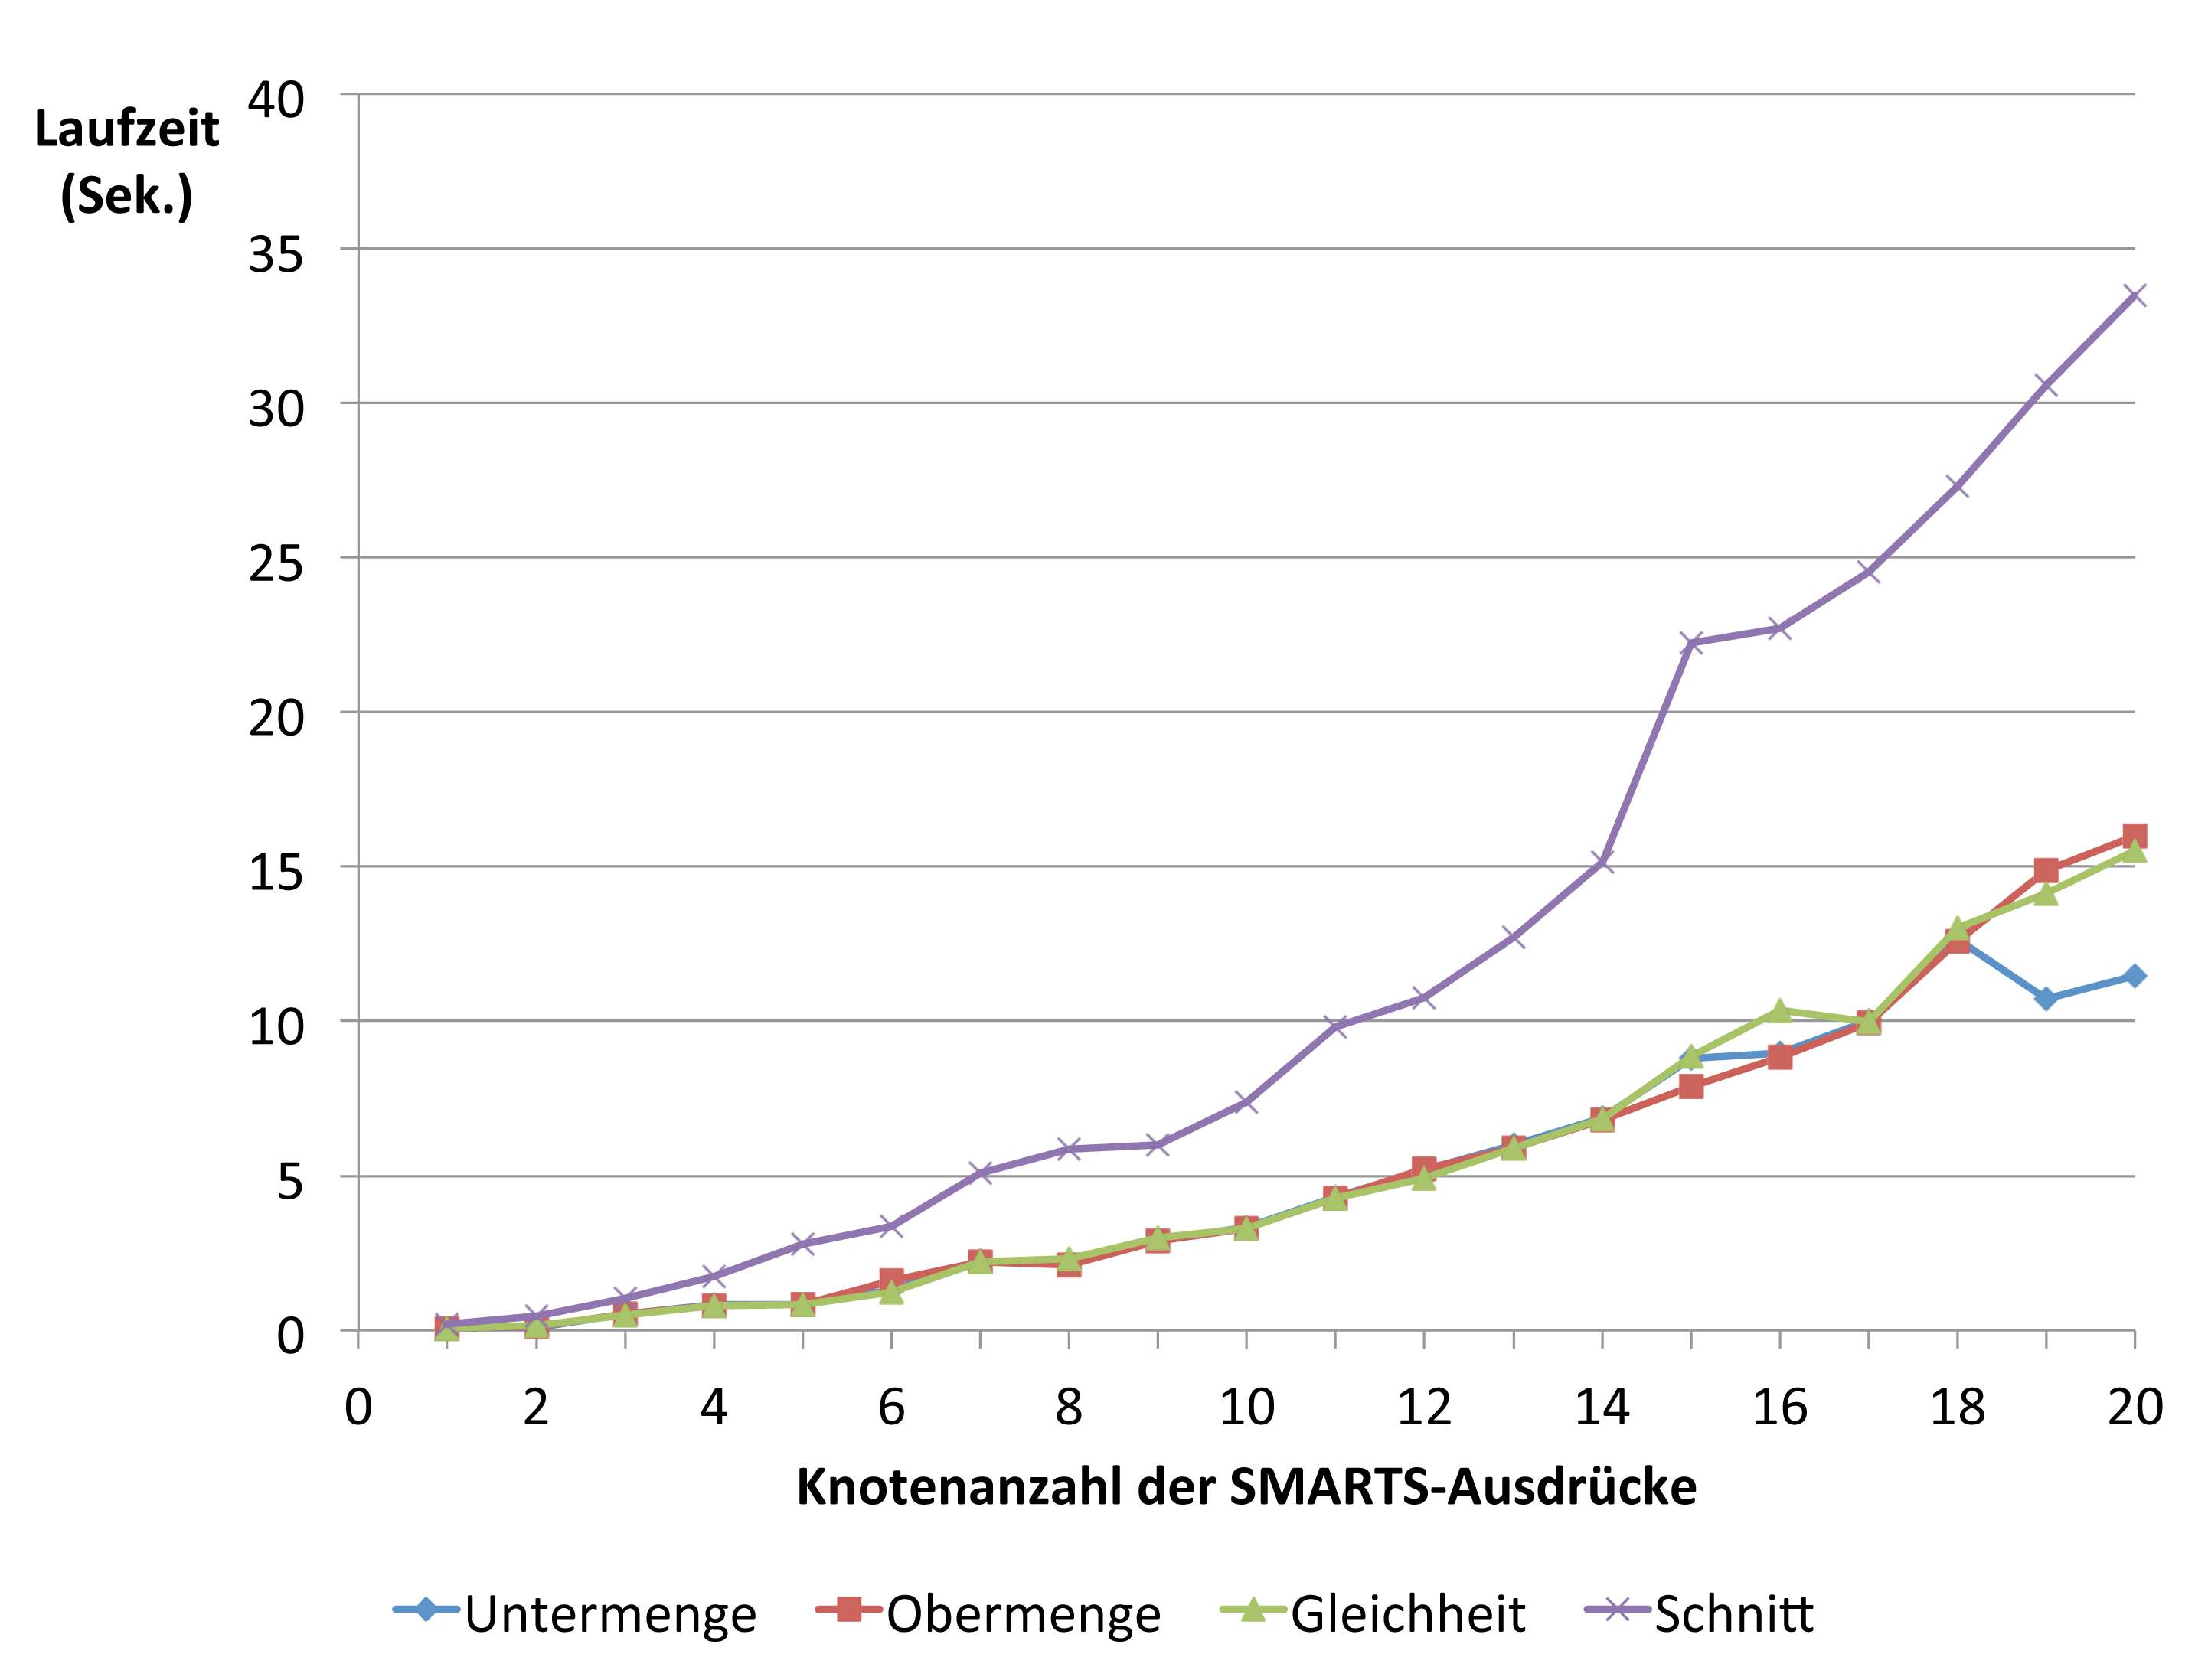
\includegraphics[width=13cm]{images/Laufzeit_gleich}
	\caption{Auftragung der Laufzeit in Sekunden, gegen Anzahl der Knoten eines SMARTS-Ausdrucks, wobei Anfrage- und Ziel-SMARTS die gleiche Gr��e besitzen. Jede Kurve repr�sentiert eine Teilmengen-Relation.}
	\label{abb:laufzeitgleich}
\end{figure}

F�r die Unter- und Obermenge l�sst sich der Fall untersuchen, bei dem die Knoten-Anzahl der SMARTS-Ausdr�cke unabh�ngig voneinander variiert. Abbildung \ref{abb:laufzeitwachs} verdeutlicht den Laufzeitanstieg (in Sekunden) bei einer ansteigenden Gr��e der Anfrage-SMARTS zusammen mit einer gleichbleibenden Gr��e der Ziel-SMARTS. Die Gr��e der gleichbleibenden SMARTS-Ausdr�cke liegt bei einer �berpr�fung auf eine Untermengen-Relation konstant bei einem Knoten. Wird auf eine Obermengen-Relation gepr�ft, so sind die SMARTS-Ausdr�cke konstant bei einer L�nge von 21 Knoten.

\newpage
\begin{figure}[h!]
	\centering
	\includegraphics[width=13cm]{images/laufzeit_wachsend}
	\caption{Auftragung der Laufzeit in Sekunden, gegen Anzahl der Knoten des Ziel-SMARTS. Der Anfrage-SMARTS besteht konstant auf einem (Untermenge) bzw. konstant auf 21 (Obermenge) Knoten.}
	\label{abb:laufzeitwachs}
\end{figure}

\vspace{0.5cm}
Diese Laufzeitanalyse l�sst  visuell auf eine lineare oder quadratische Laufzeit schlie�en. Der genutzte Algorithmus nach Ullmann ben�tigt im schlimmsten Fall, bei einem Anfrag-SMARTS mit Knotenanzahl $n$ und einem Ziel-SMARTS mit Knotenanzahl $m$, eine Laufzeit, die in $\mathcal{O}(m^nn^2)$ liegt. Bei dem Aufbau der Relations-Matrix werden $nm$ Vergleiche, und bei dem Aufbau der Kanten-Vertr�glichkeit $(n-1)(m-1)$ Vergleiche ben�tigt. Letztendlich liegt die Laufzeit des entwickelten Verfahrens im schlimmsten Fall in $\mathcal{O}(m^nn^2)$.
%
% EOF
%
%
% Diskussion und Bewertung
%
\section{Experimente und Auswertung}\label{sec:experimente}
Nach Abschluss der Validierung wurde das vorgestellte und implementierte Verfahren auf echten Daten getestet, die einen m�glichen Anwendungsbereich des Verfahrens darstellen. In dem hier vorgestellten Experimenten handelt es sich um einen Anwendungsbereich, bei dem Filter, bestehend aus SMARTS-Ausdr�cken, auf �berlappungen �berpr�ft werden. Es wurden acht verschiedene SMARTS-Filter miteinander zu verglichen. Diese Filter wurden von im Rahmen der Datenbank ChEMBL \cite{ChEMBL}\cite{ChEMBLrelease}\cite{ChEMBLpersonal} aus den folgenen Quellen zusammengetragen:
\begin{enumerate}
	\item Bristol-Myers Squibb HTS Deck Filters (\textbf{BMS})
	\item University of Dundee NTD Screening Library Filters (\textbf{Dundee})
	\item Glaxo Wellcome Hard Filters (\textbf{Glaxo})
	\item Inpharmatica Unwanted Fragments (\textbf{Inpharmatica})
	\item Pfizer LINT filters (\textbf{LINT})
	\item NIH MLSMR Excluded Functionality Filters (\textbf{MLSMR})
	\item Pan Assay Interference Compounds Filters (\textbf{PAINS})
	\item SureChEMBL Data (\textbf{SureChEMBL})
\end{enumerate} 

Die gewonnenen Listen wurden von Christian Laggner auf falsche SMARTS-Ausdr�cke untersucht und diese korrigiert (siehe Anhang \ref{ssec:experiments}).
Diese Sammlungen von SMARTS-Ausdr�cken werden als sogenannte \textit{structural alerts} eingesetzt. \textit{Structural alerts} werden genutzt um unter Umst�nden problematische Molek�le bei der Wirkstoffentwicklung herauszufiltern. So werden Molek�le mit toxikologisch Substrukturen oder funktionellen Gruppen ausgefiltert, aber auch bekannte instabile Molek�le, Molek�le, die bei Tests st�ren k�nnten und welche, die beim HTS (\textit{High throughput Screening}) \cite{chemoinformatik} h�ufige Treffer darstellen. \cite{ChEMBLrelease}\\

\begin{table}[h]
	\centering
	\captionabove{Anzahl der SMARTS-Ausdr�cke pro \textit{structural alert}-Filter vor und nach der �bergabe an das Programm \textit{SmartsSmarts} (siehe Kapitel \ref{ssec:vorverarbeitung}).}
	\begin{tabular}{| l | l | l |}
		\hline Filter-Set & Anzahl & nach �bergabe\\
		& SMARTS-Ausdr�cke & an \textit{SmartsSmarts}\\
		\hline BMS & 180 & 87\\
		Dundee & 105 & 100\\
		Glaxo & 55 & 54\\
		Inpharmatica & 92 & 83\\
		LINT & 58 & 48\\
		MLSMR & 116 & 105\\
		PAINS & 481 & 423\\
		SureChEMBL & 166 & 148\\ \hline
	\end{tabular}
	\label{tab:experiments}
\end{table}

\newpage
\begin{figure}[h!]
\fbox{\begin{minipage}{16cm}
	\begin{center}
	\begin{minipage}{5cm}
		\centering
		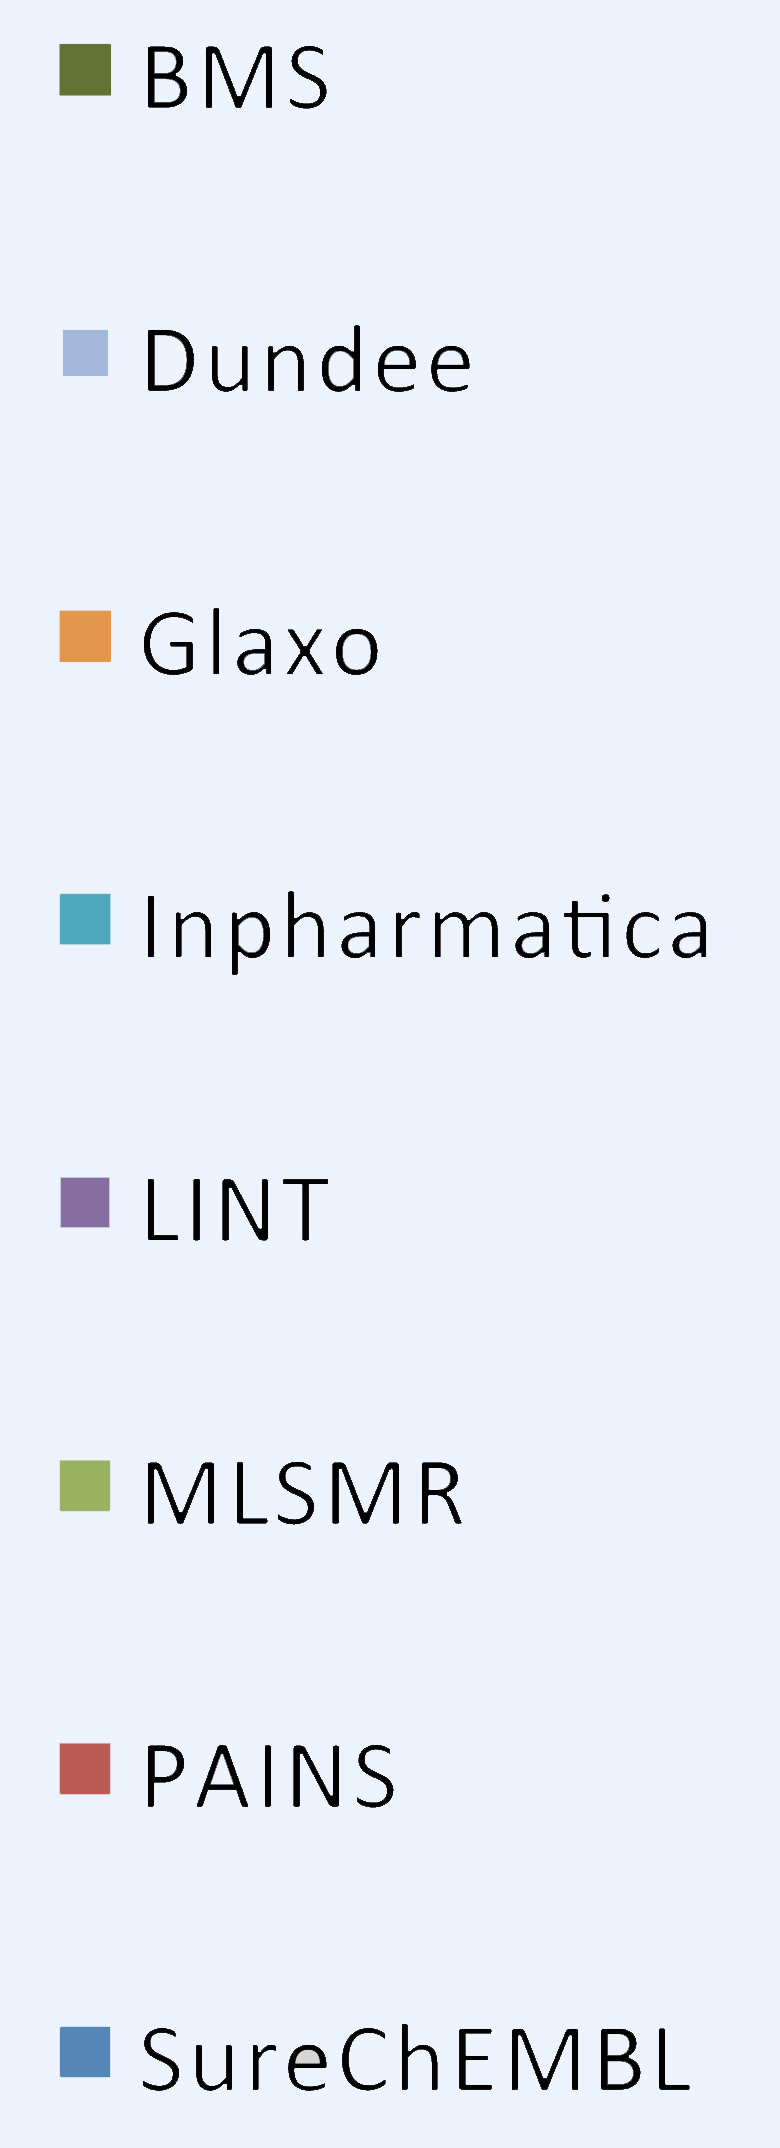
\includegraphics[width=3cm]{images/Legende3}
	\end{minipage}
	\begin{minipage}{5cm}
		\centering
		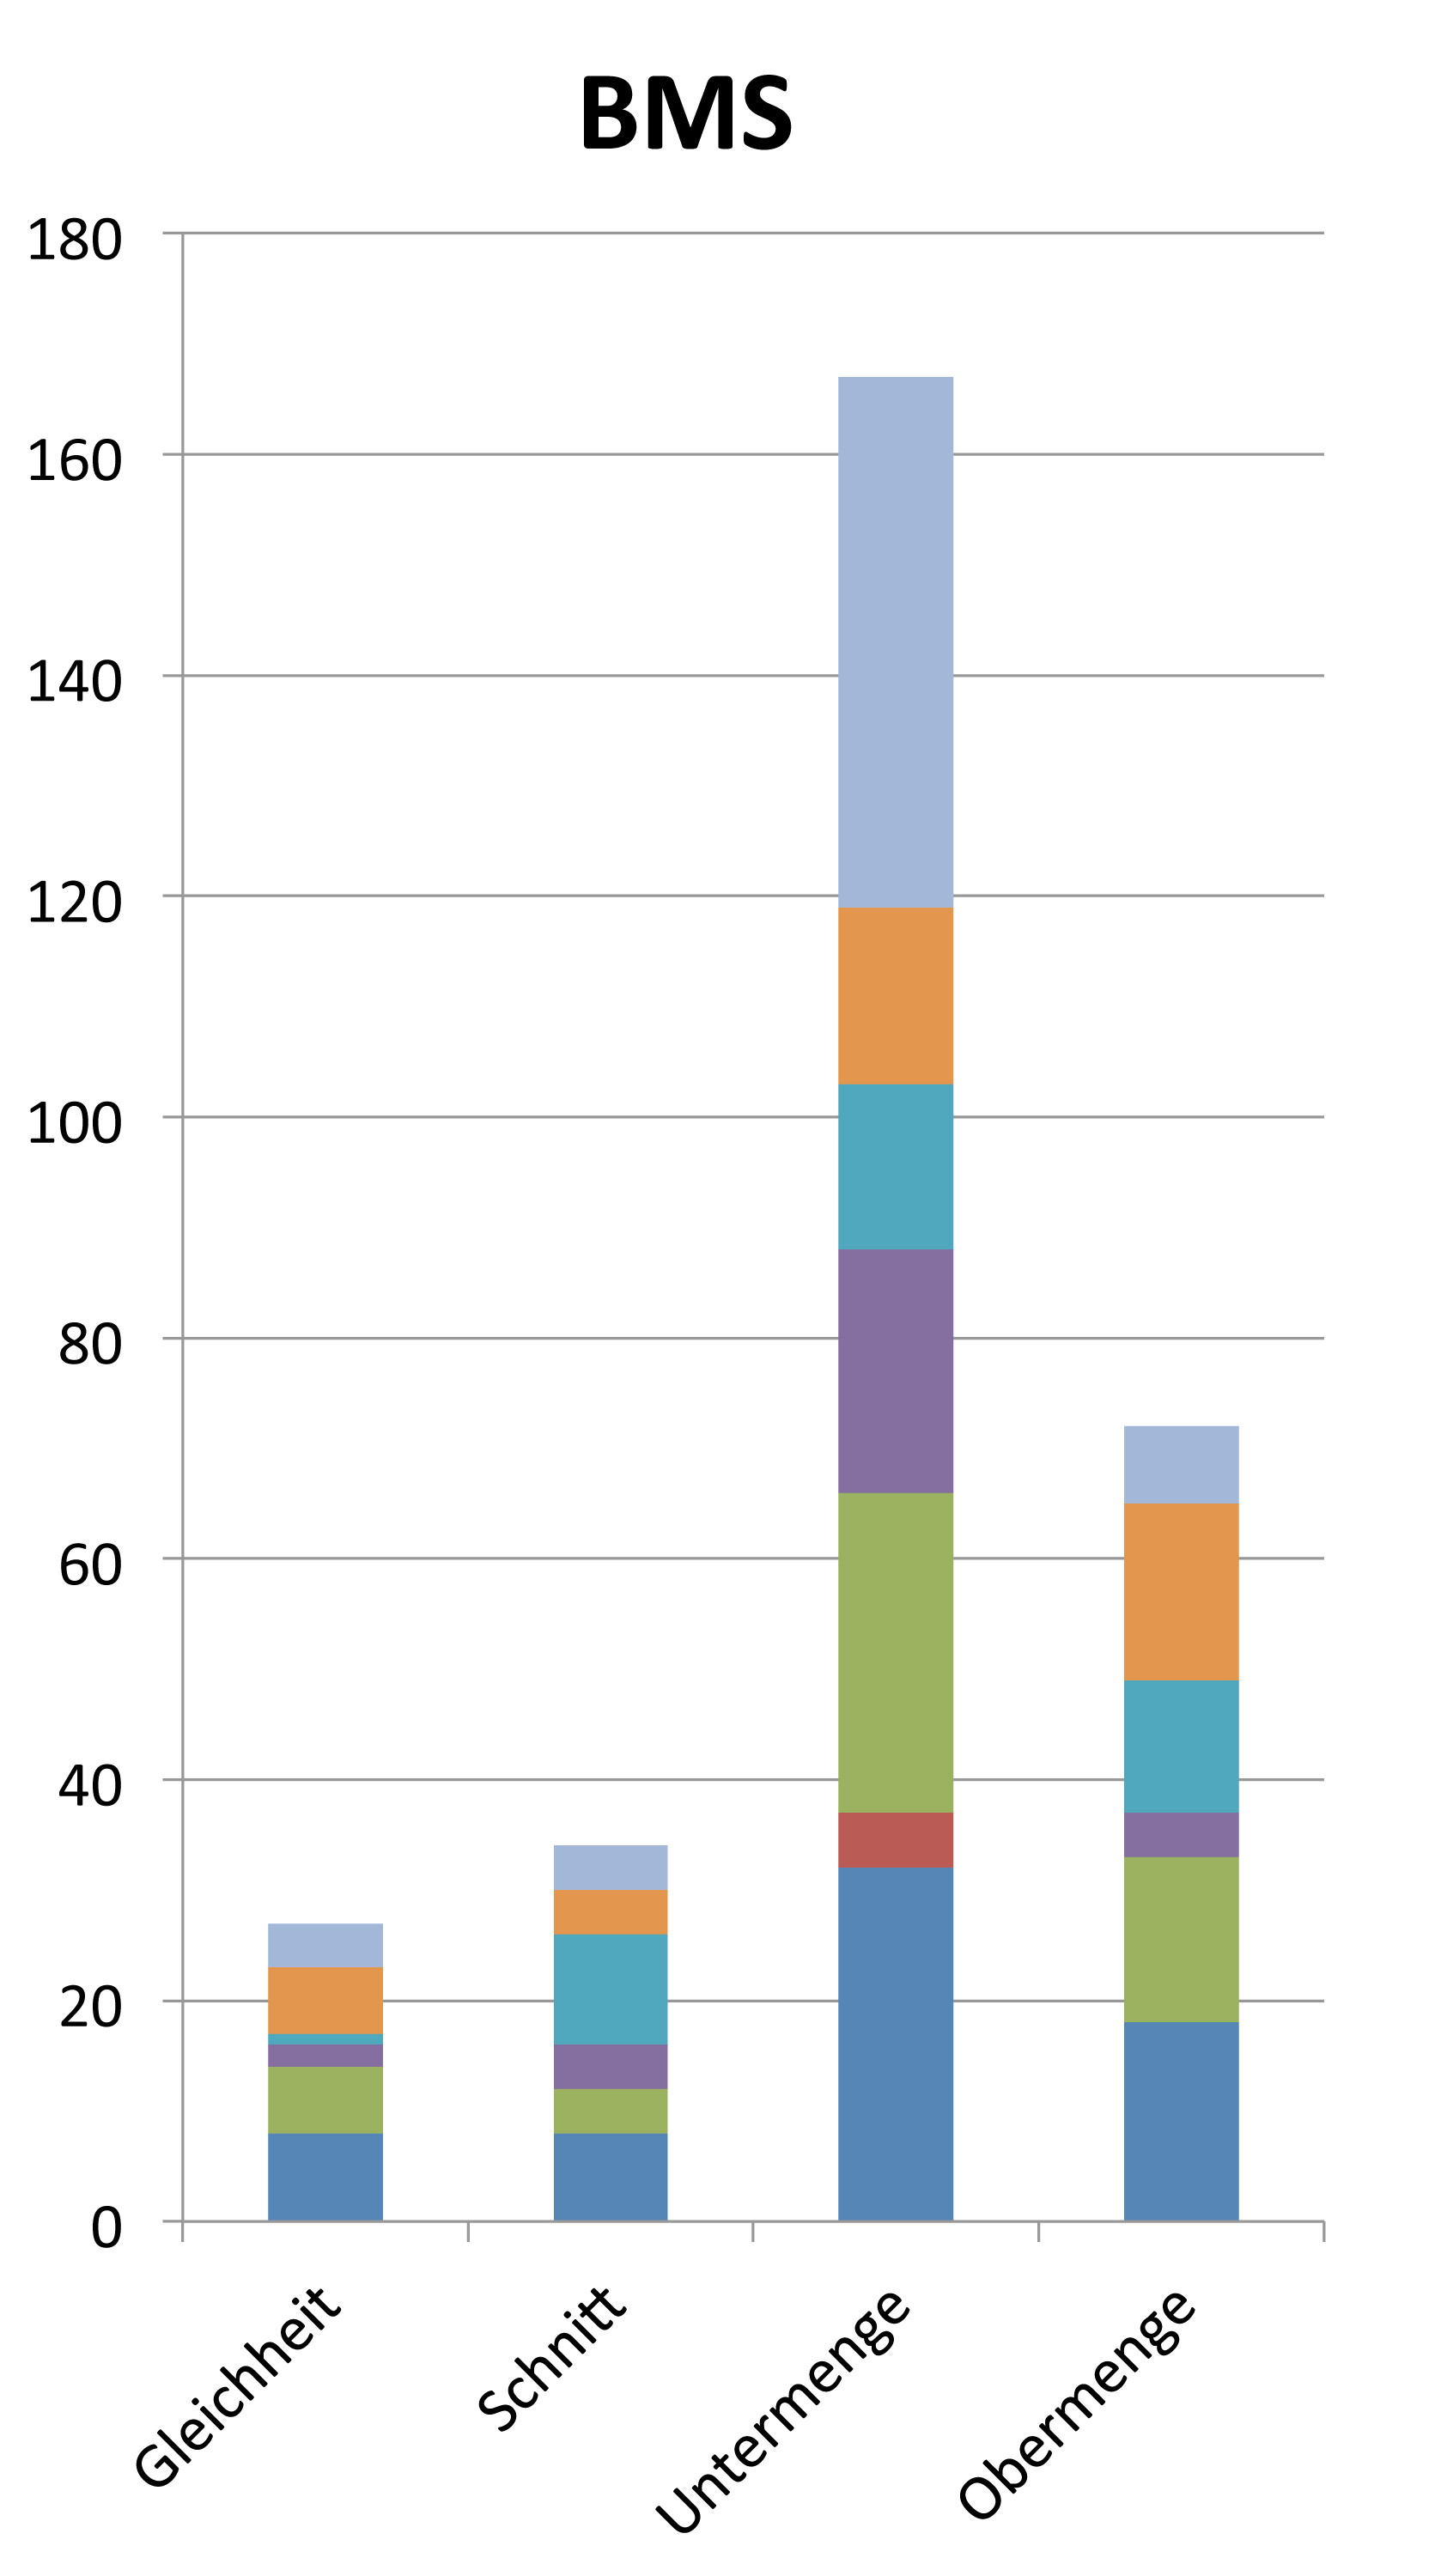
\includegraphics[width=5cm]{images/BMS}
	\end{minipage}
	\begin{minipage}{5cm}
		\centering
		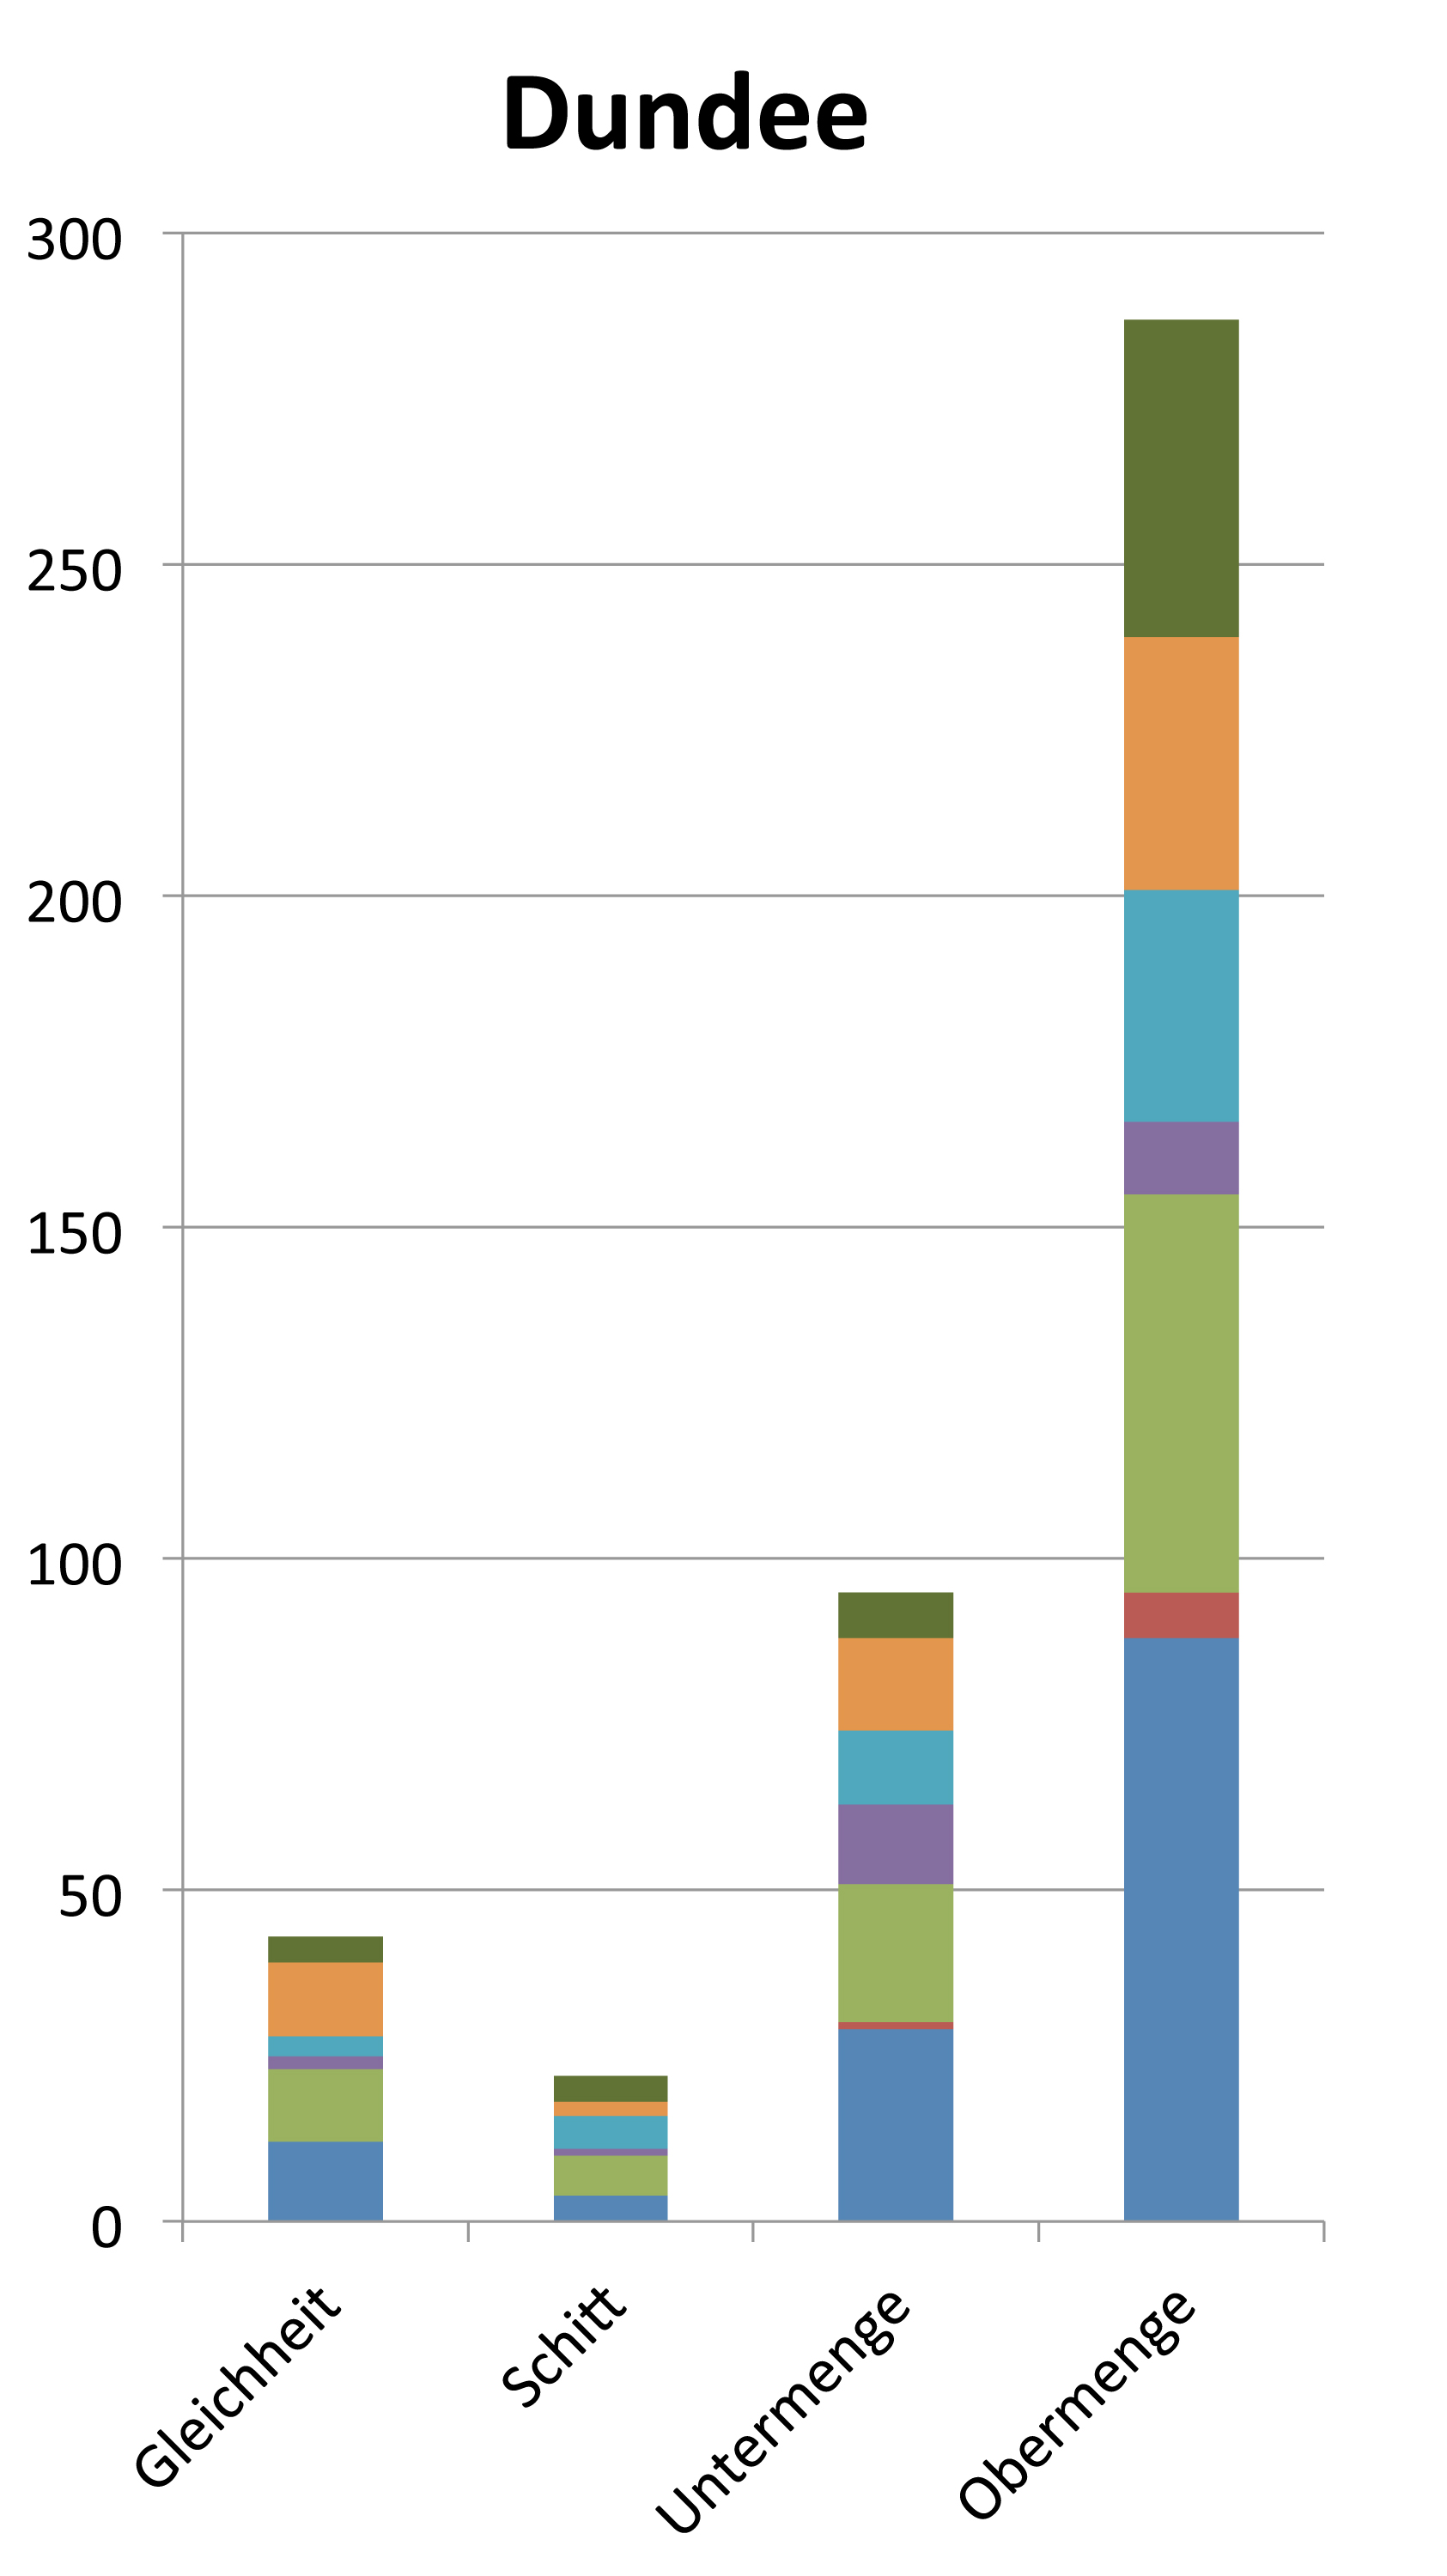
\includegraphics[width=5cm]{images/Dundee}
	\end{minipage}
\begin{center}
	\begin{minipage}{7cm}
		\centering
		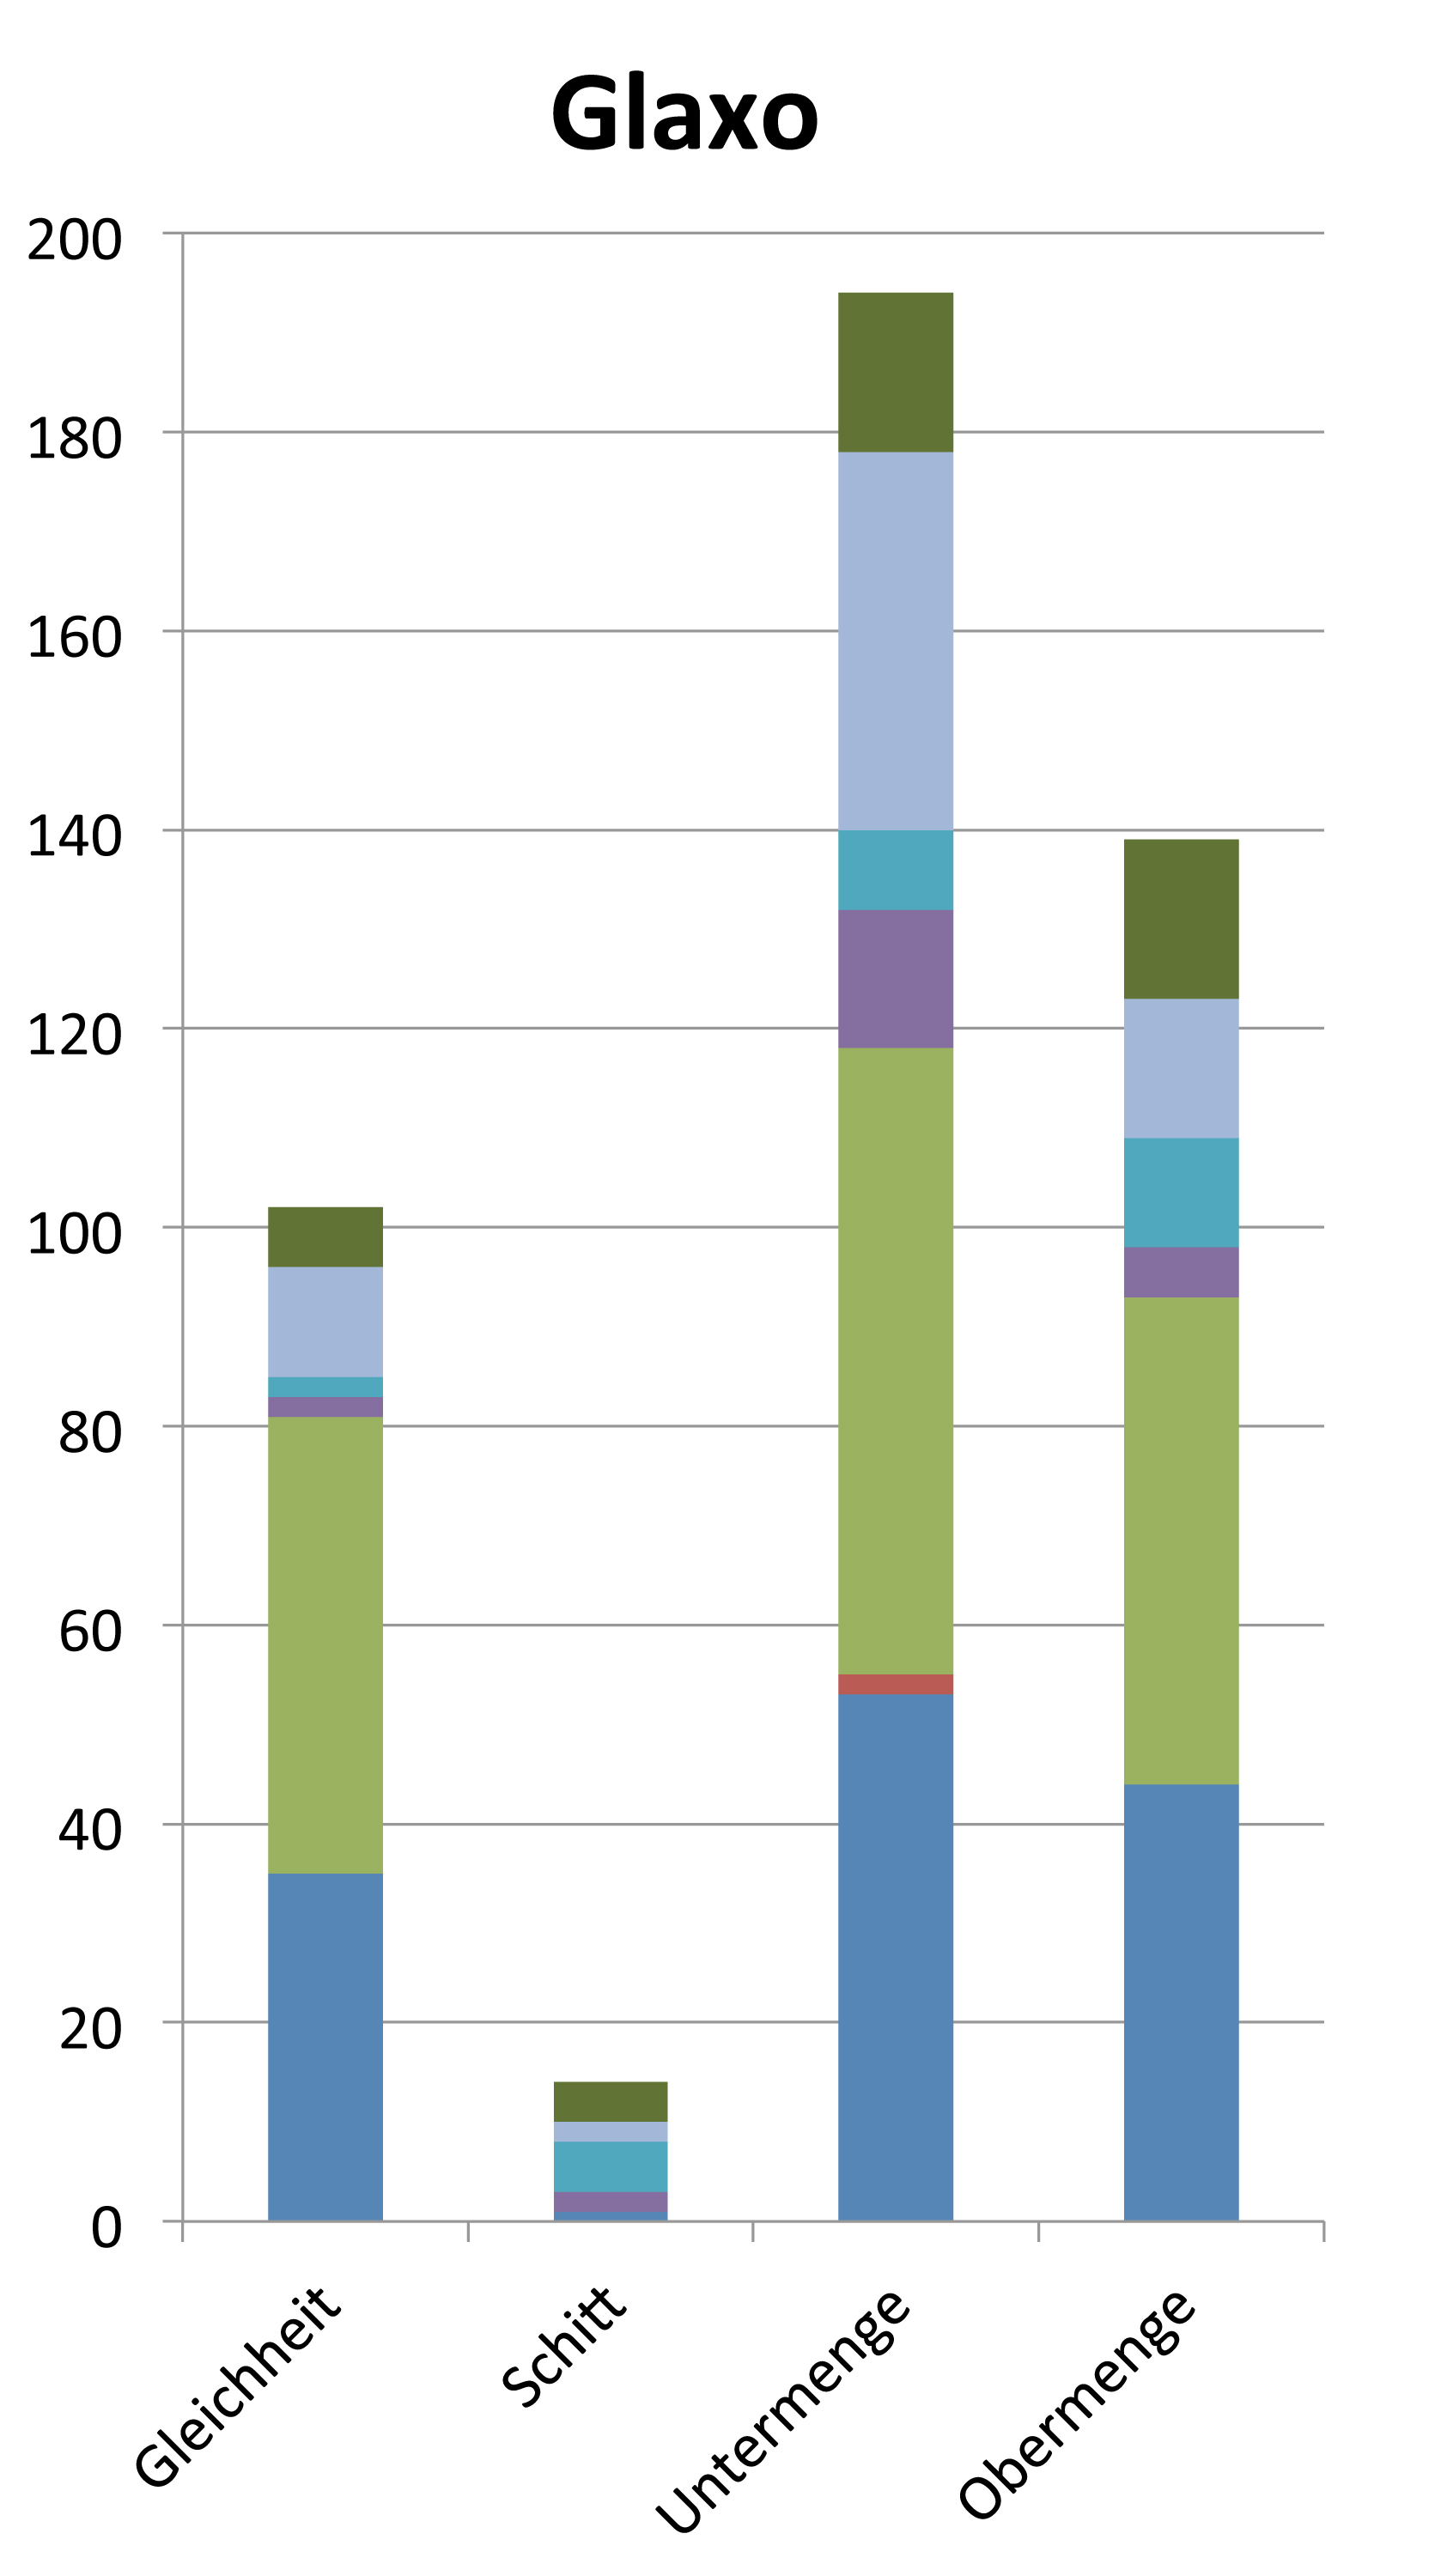
\includegraphics[width=5cm]{images/Glaxo}
	\end{minipage}
	\begin{minipage}{7cm}
		\centering
		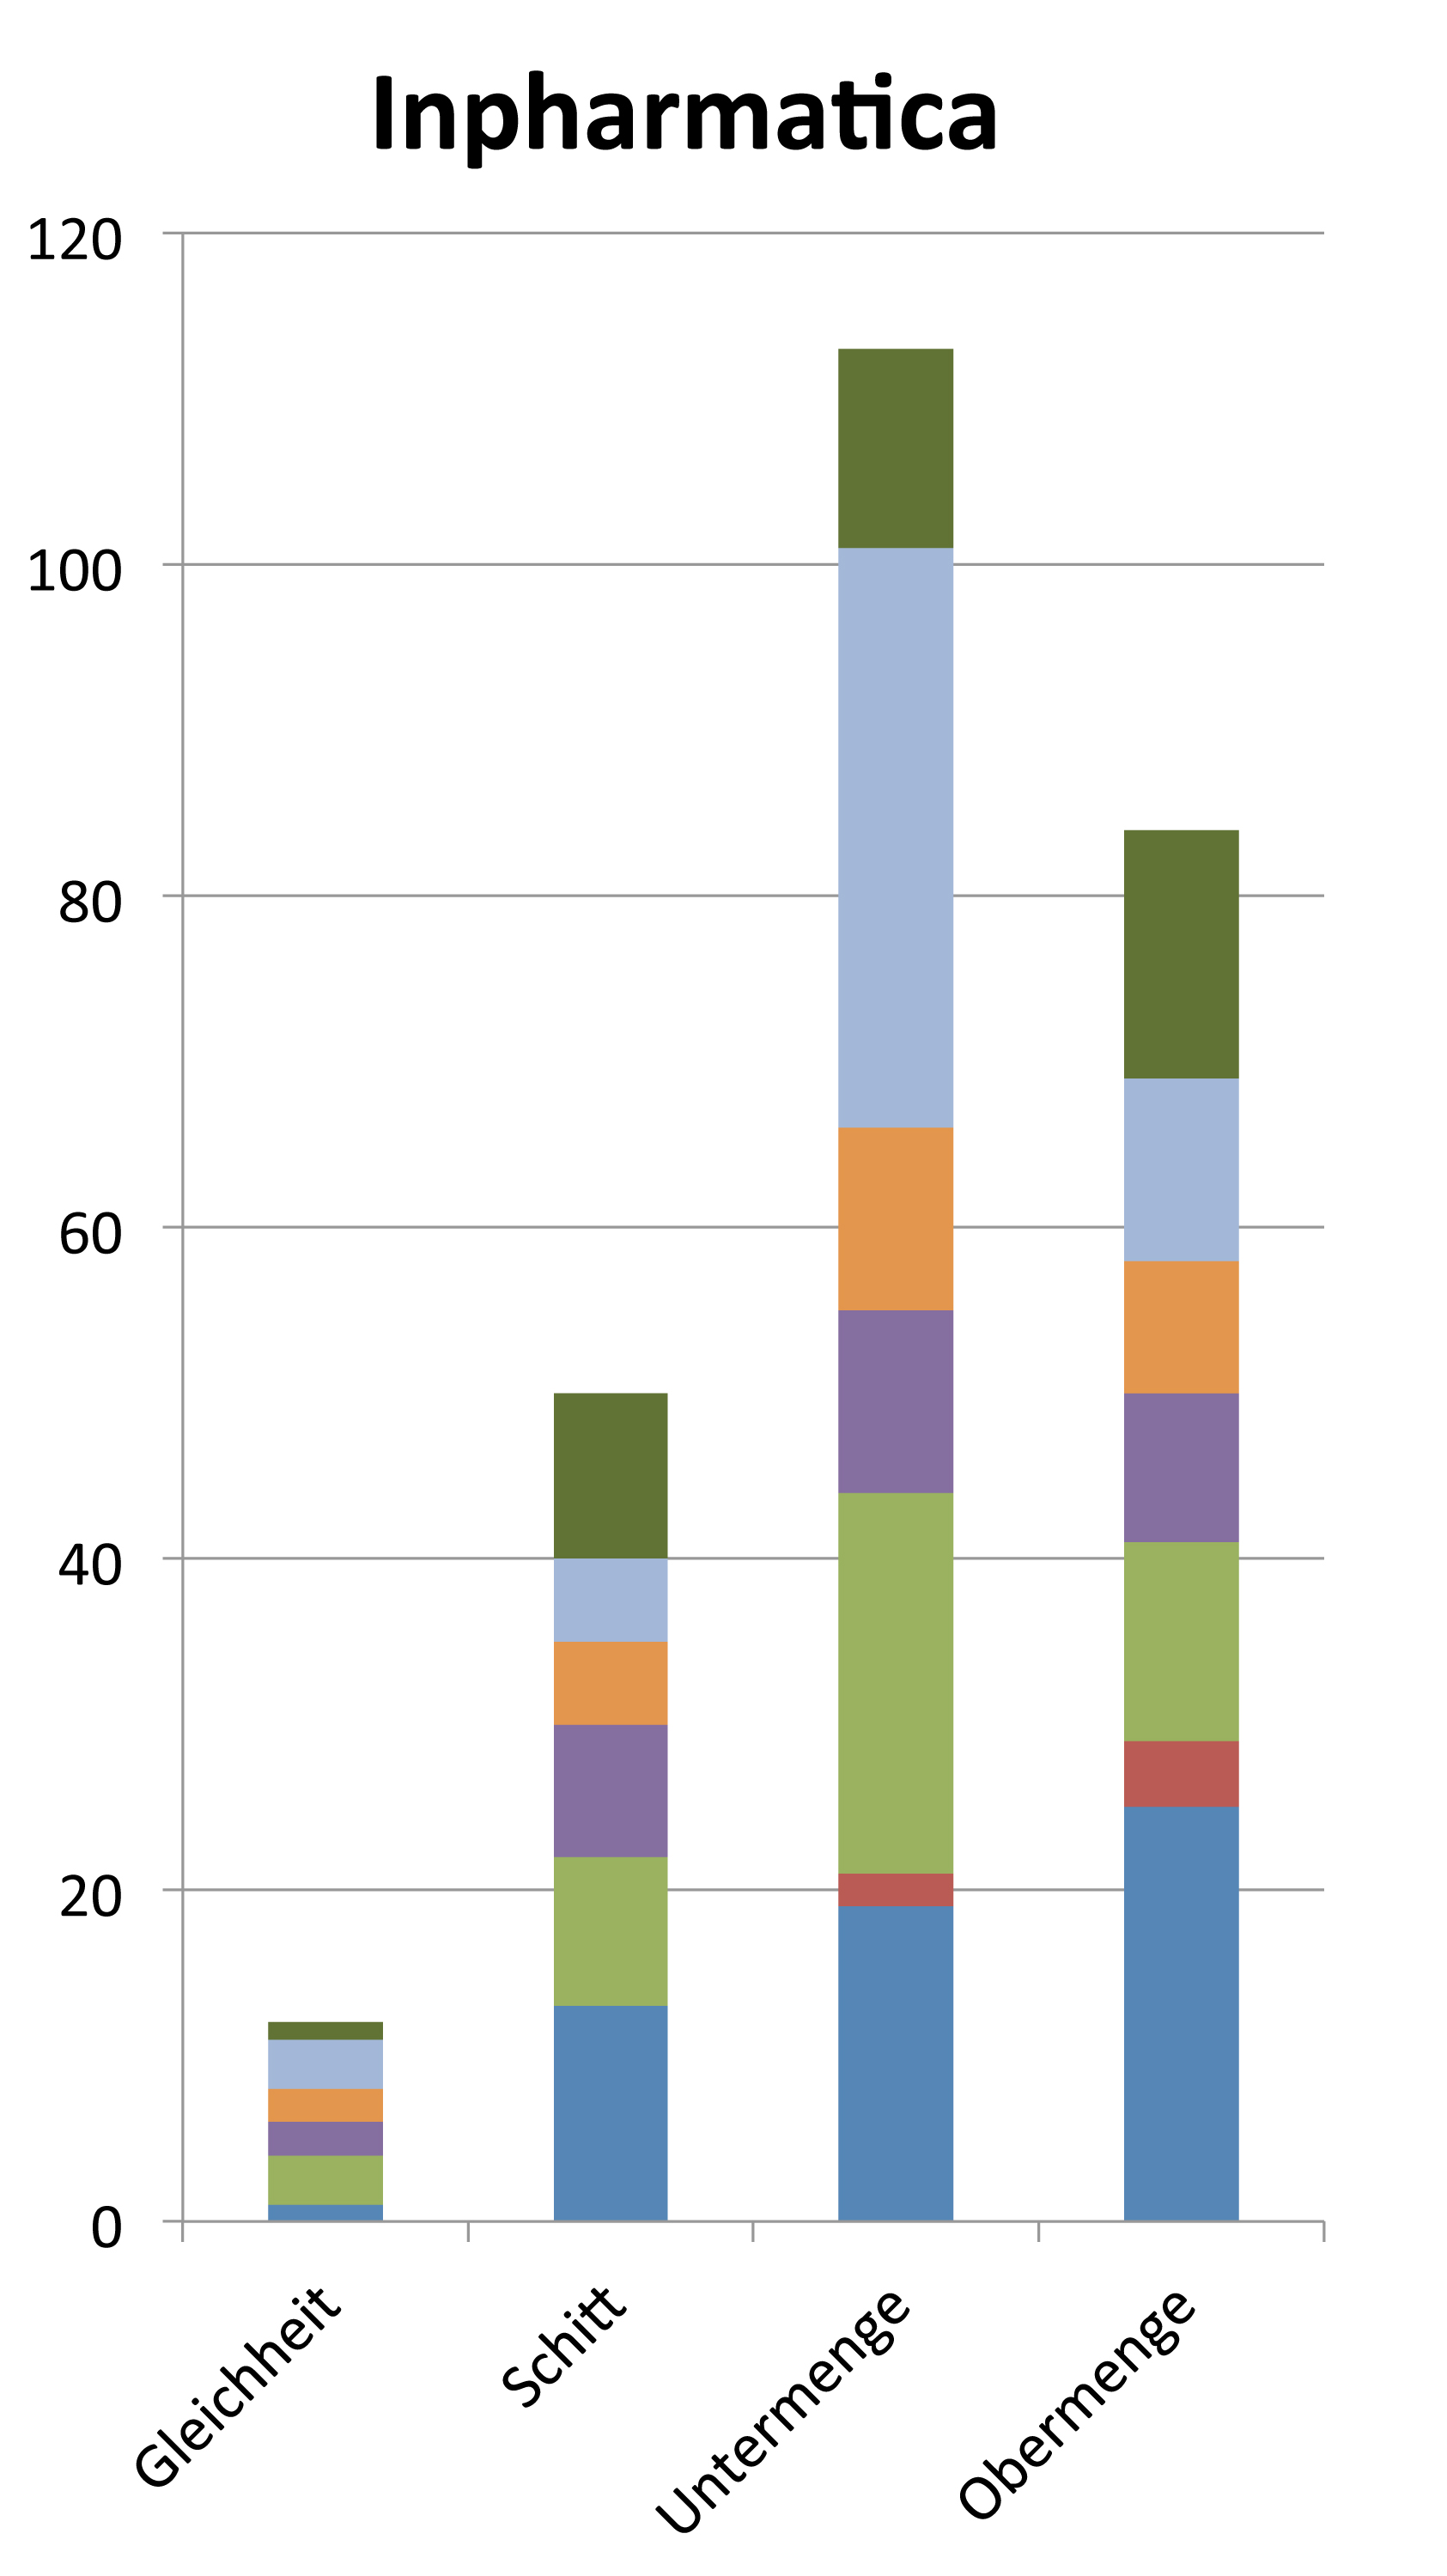
\includegraphics[width=5cm]{images/Inpharmatica}
	\end{minipage}
	\end{center}
\end{center}
\end{minipage}}
\caption{Erster Teil der Experimente: Dargestellt ist f�r wie viele Ziel-SMARTS ein \textit{Mapping} zu den Anfrage-SMARTS der einzelnen SMARTS-Filter (BMS, Dundee, Glaxo und Inpharmatica) gefunden wurde. Die \textit{Mappings} sind Farbig markiert, je nachdem aus welchen anderen Filtern sie stammen. Zu beachten sind die unterschiedlichen Skalierungen (vgl. Tabelle \ref{tab:experiments}).}
\label{abb:experiments1}
\end{figure}

\newpage
\subsection{Diskussion der Experimente}
Anhand der Ergebnisse, die f�r die Vergleiche der SMARTS-Filter gewonnen wurden, k�nnen R�ckschl�sse auf die Art der \textit{structural alters} gezogen werden. Im Folgenden wird auf die Ergebnisse von jedem Filter eingegangen. Zudem wird anschlie�end ein chemisches Muster gezeigt, welches in jedem Filter (ohne PAINS) in einer allgemeinen, oder spezifizierten Form vorlag.

\textbf{BMS} (vgl. Abbildung \ref{abb:experiments1})\\
Nach Durchf�hrung der Vergleiche von dem Filter BMS mit allen anderen Filtern wird deutlich, dass bei den Vergleichen vor allem eine Untermengen-Relation festgestellt wurde. Es l�sst darauf schlie�en, dass BMS im Vergleich zu den anderen (insbesondere zu Dundee) Filter nutzt, die spezifizierter eingesetzt werden.

\textbf{Dundee} (vgl. Abbildung \ref{abb:experiments1})\\
Durch die vorgehende Pr�fung auf Redundanz wurde bei dem Filter Dundee ein redundantes Muster festgestellt. Bei Dundee l�sst sich das Gegenteil zu BMS feststellen. So sind die Filter aus diesem Set allgemeiner gehalten. In Anbetracht der Anzahl der SMARTS-Ausdr�cke wurde eine gro�e Menge SMARTS-Ausdr�cken gefunden, f�r die eine Obermengen-Relation festgestellt werden konnte.

\textbf{Glaxo} (vgl. Abbildung \ref{abb:experiments1})\\
Bei den Vergleichen mit dem Set von Glaxo wurden �ber 100 \textit{Mappings} gefunden, die eine Gleichheit darstellen. Da der Glaxo-Filter mit 54 brauchbaren SMARTS-Ausdr�cken eine relativ geringe Gr��e hat, deutet die gro�e Anzahl der \textit{Mappings} darauf hin, dass dieser Filter SMARTS-Ausdr�cke benutzt, die in �hnlicher Form in den meisten anderen Filtern vorkommt.

\textbf{Inpharmatica} (vgl. Abbildung \ref{abb:experiments1})\\
F�r Inpharmatica wurden beinahe ausgewogen Ober- und Untermengen-\textit{Mappings gefunden}. Besonders auff�llig ist die hohe Anzahl von Ziel-SMARTS, f�r die ein \textit{Mapping} der Schnitt-Relation gefunden wurde. Zur�ckzuf�hren l�sst sich dieses Verhalten darauf, dass die SMARTS-Ausdr�cke, die der Filter Inpharmatica nutzt, h�ufig Teilstrukturen besitzen die allgemeiner sind, sowie welche die spezifischer sind.

\textbf{LINT} (vgl. Abbildung \ref{abb:experiments2})\\
Anhand der Ergebnisse der Vergleiche mit dem SMARTS-Filter LINT kann davon ausgegangen werden, dass die genutzten SMARTS-Ausdr�cke gr��tenteils allgemeiner gehalten sind. Da der SMARTS-Filter nur 48 SMARTS-Ausdr�cke nutzt und somit der kleinste Filter ist konnte mit diesem Ergebnis gerechnet werden.

\textbf{MLSMR} (vgl. Abbildung \ref{abb:experiments2})\\
�hnlich zu dem SMARTS-Filter Inpharmatica wurde auch bei dem Filter MLSMR eine Ausgewogenheit von gefundenen \textit{Mappings} zwischen Unter- und Obermenge festgestellt. Zudem wurde zu �ber 100 Ziel-SMARTS eine Gleichheit-Relation festgestellt. MSLSMR scheint damit einen SMARTS-Filter zu nutzen, der einen guten Repr�sentanten der anderen Filter darstellen k�nnte.

\begin{figure}[h!]
\fbox{\begin{minipage}{16cm}
	\begin{center}
		\begin{minipage}{5cm}
			\centering
			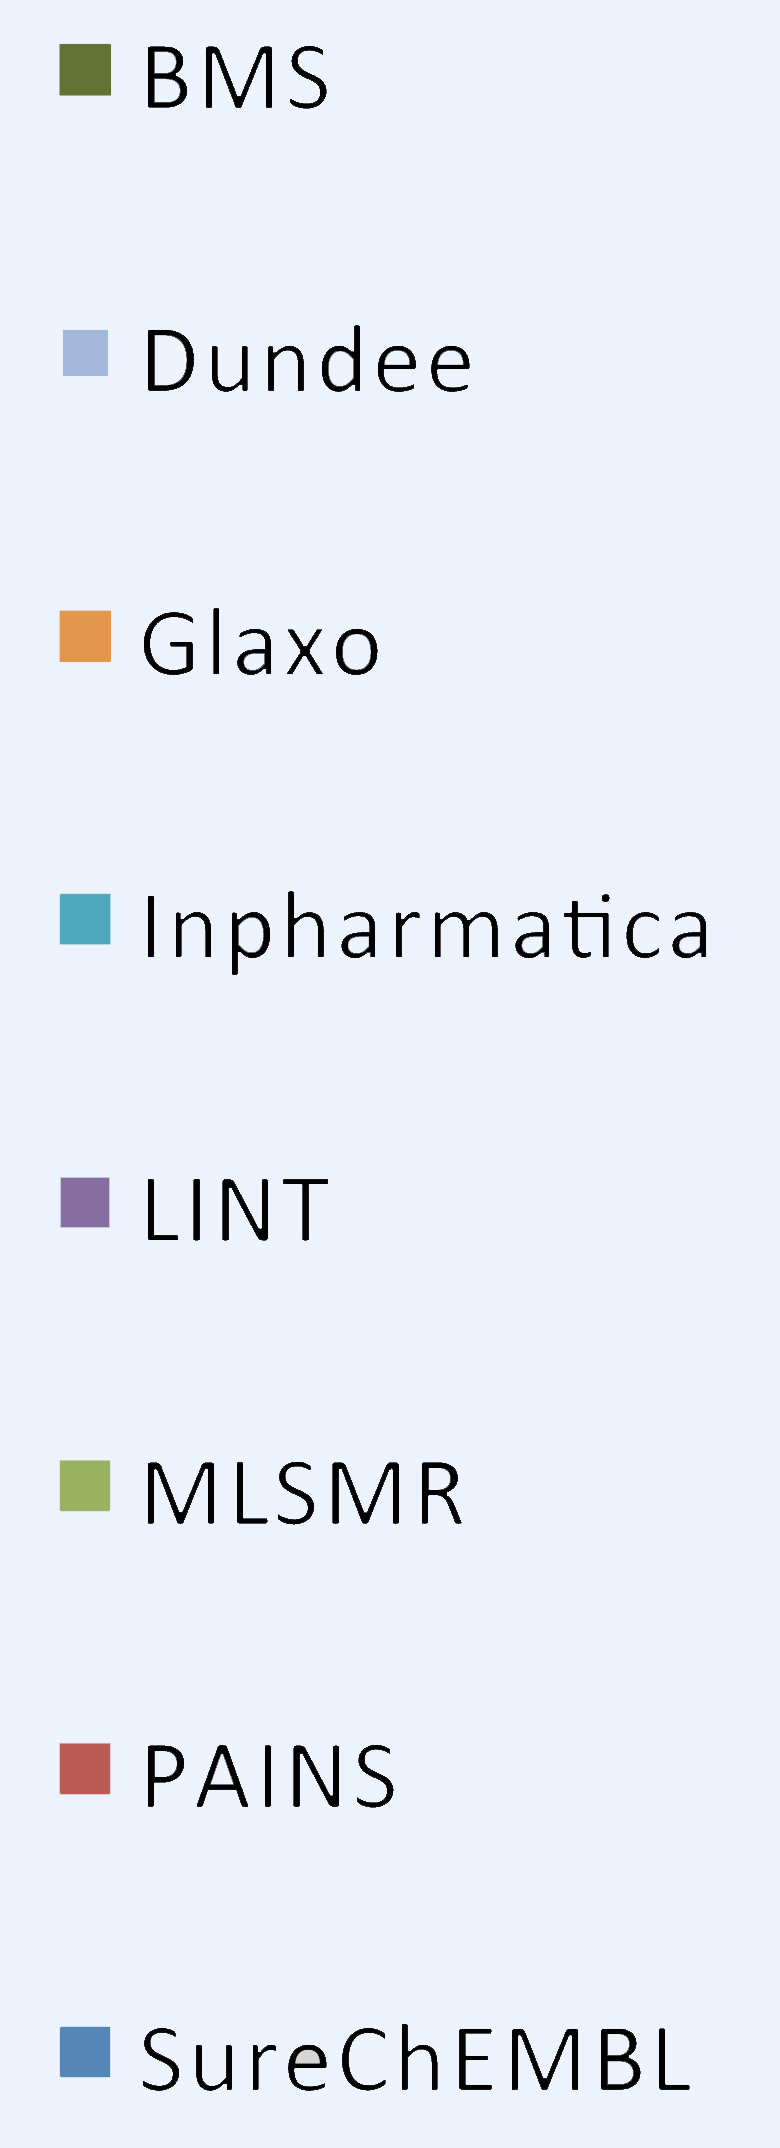
\includegraphics[width=3cm]{images/Legende3}
		\end{minipage}
		\begin{minipage}{5cm}
			\centering
			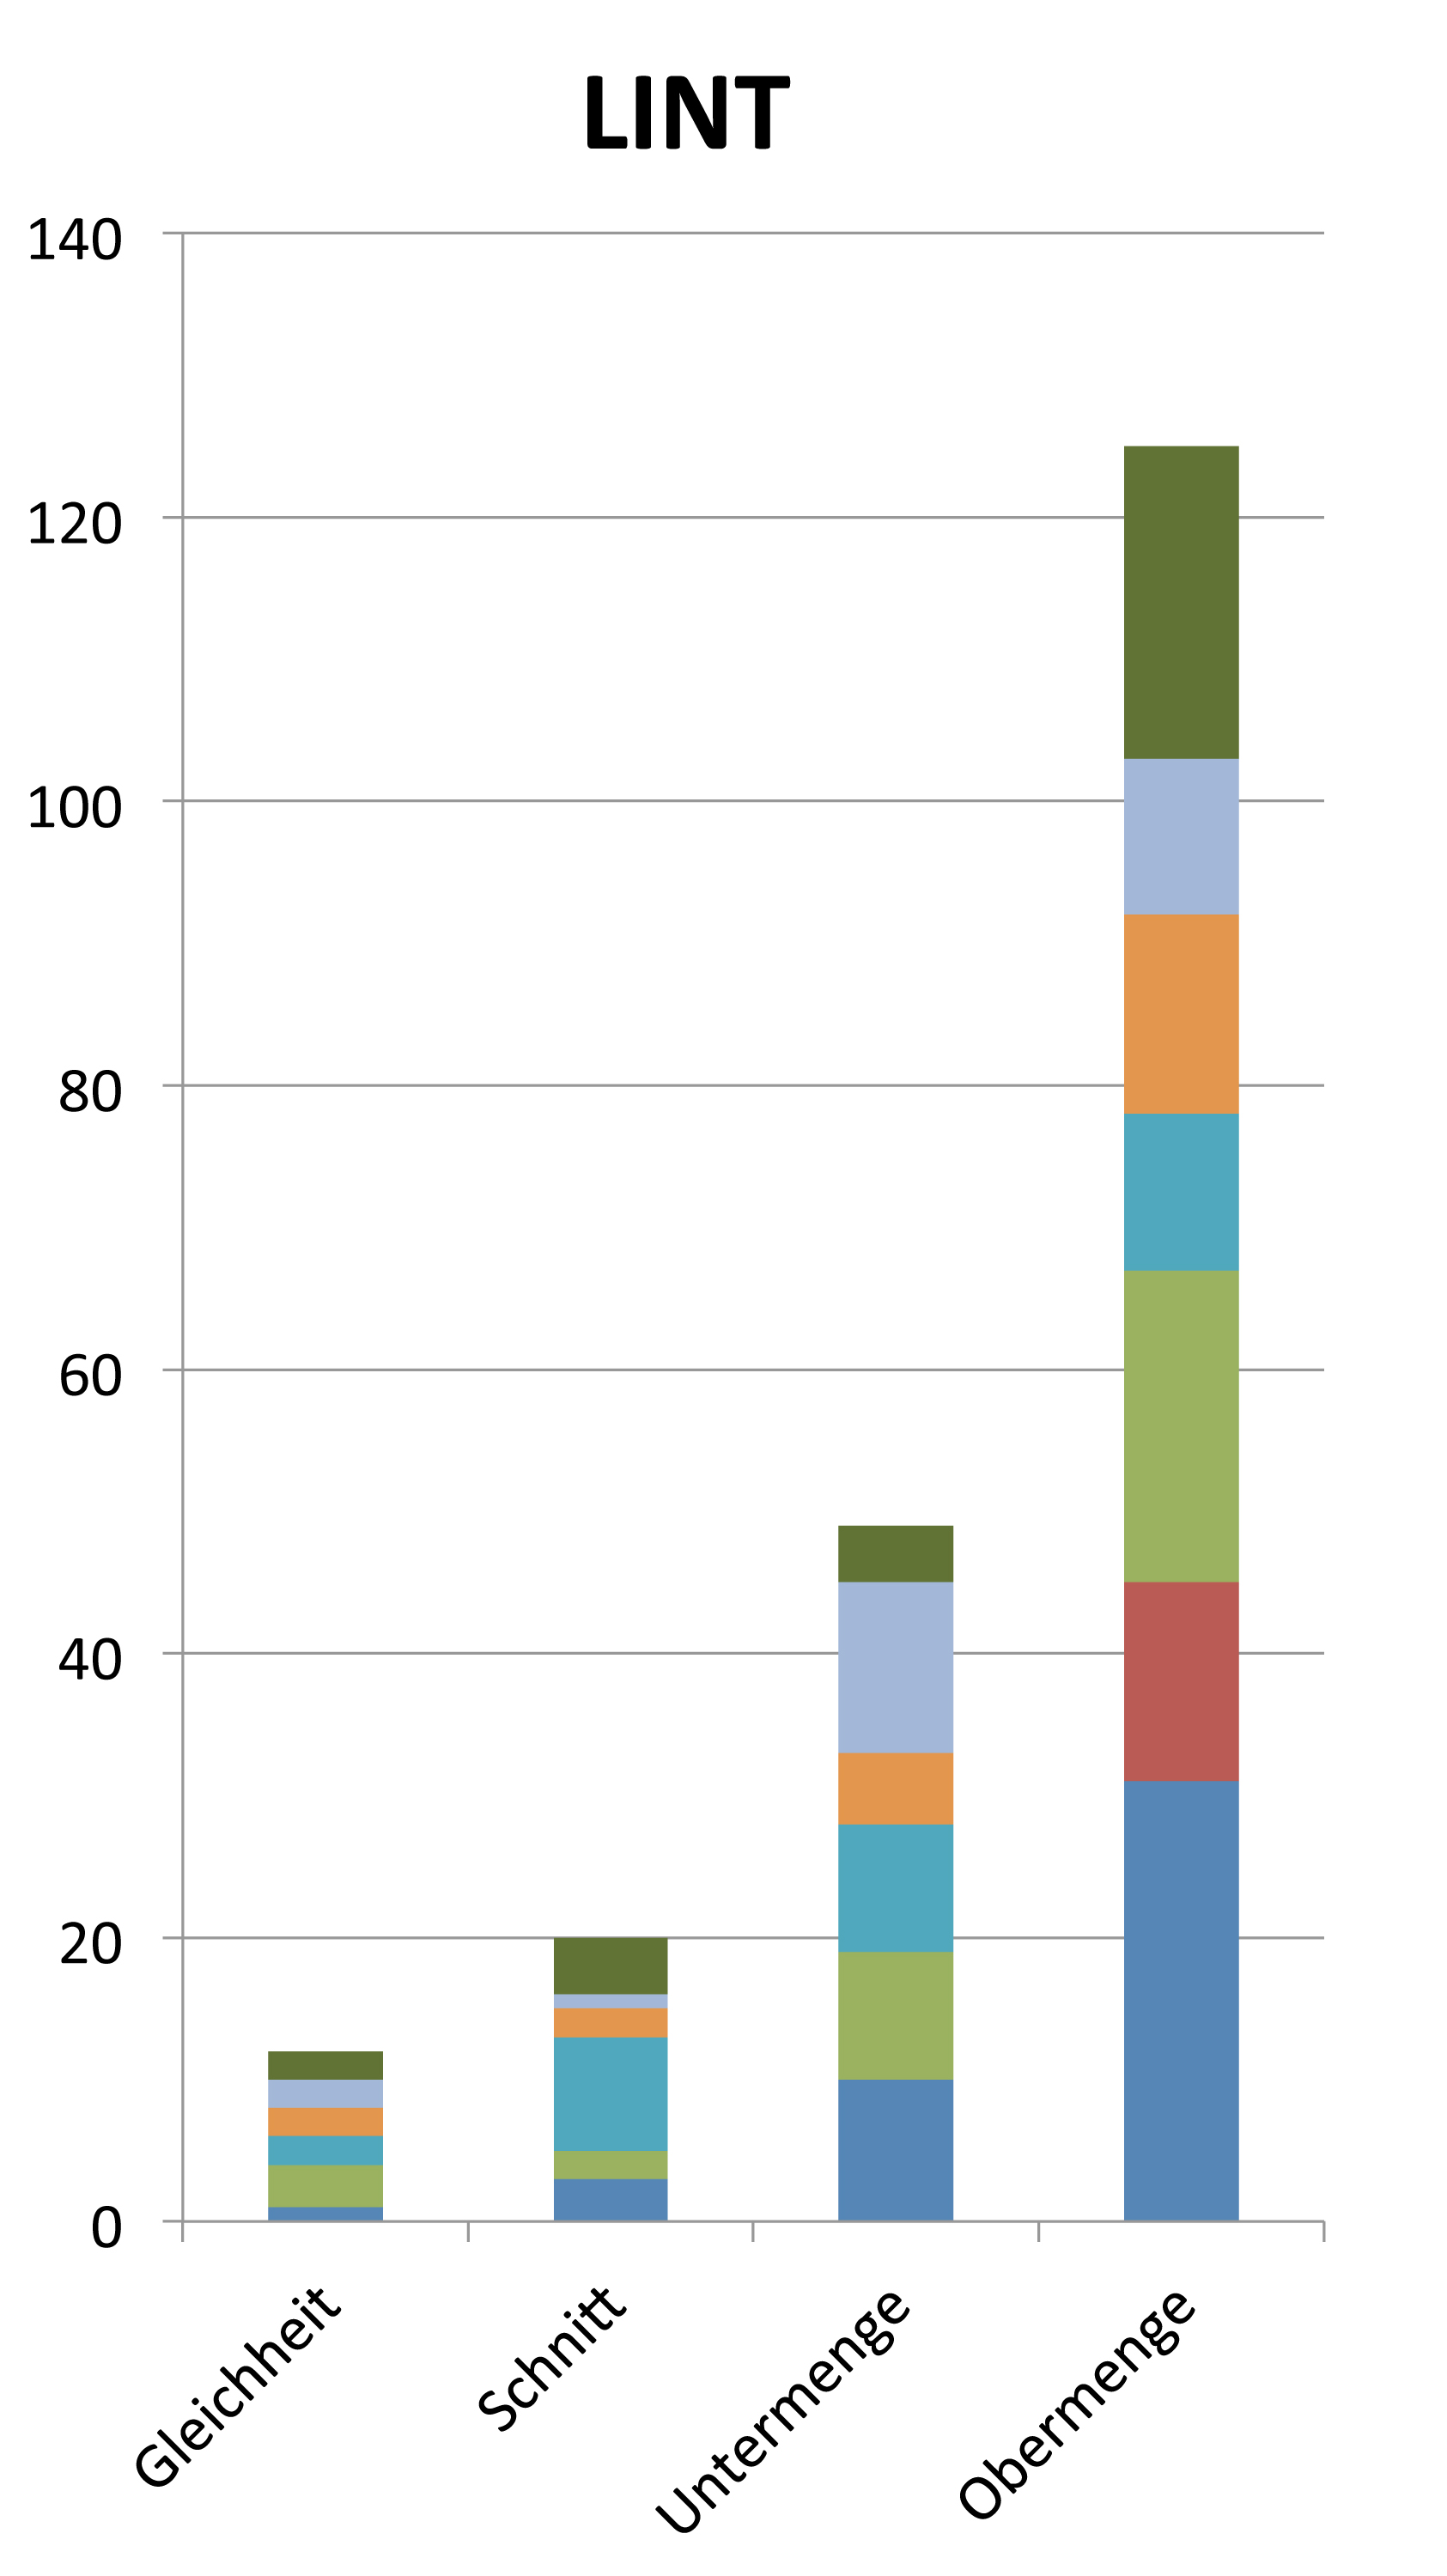
\includegraphics[width=5cm]{images/LINT}
		\end{minipage}
		\begin{minipage}{5cm}
			\centering
			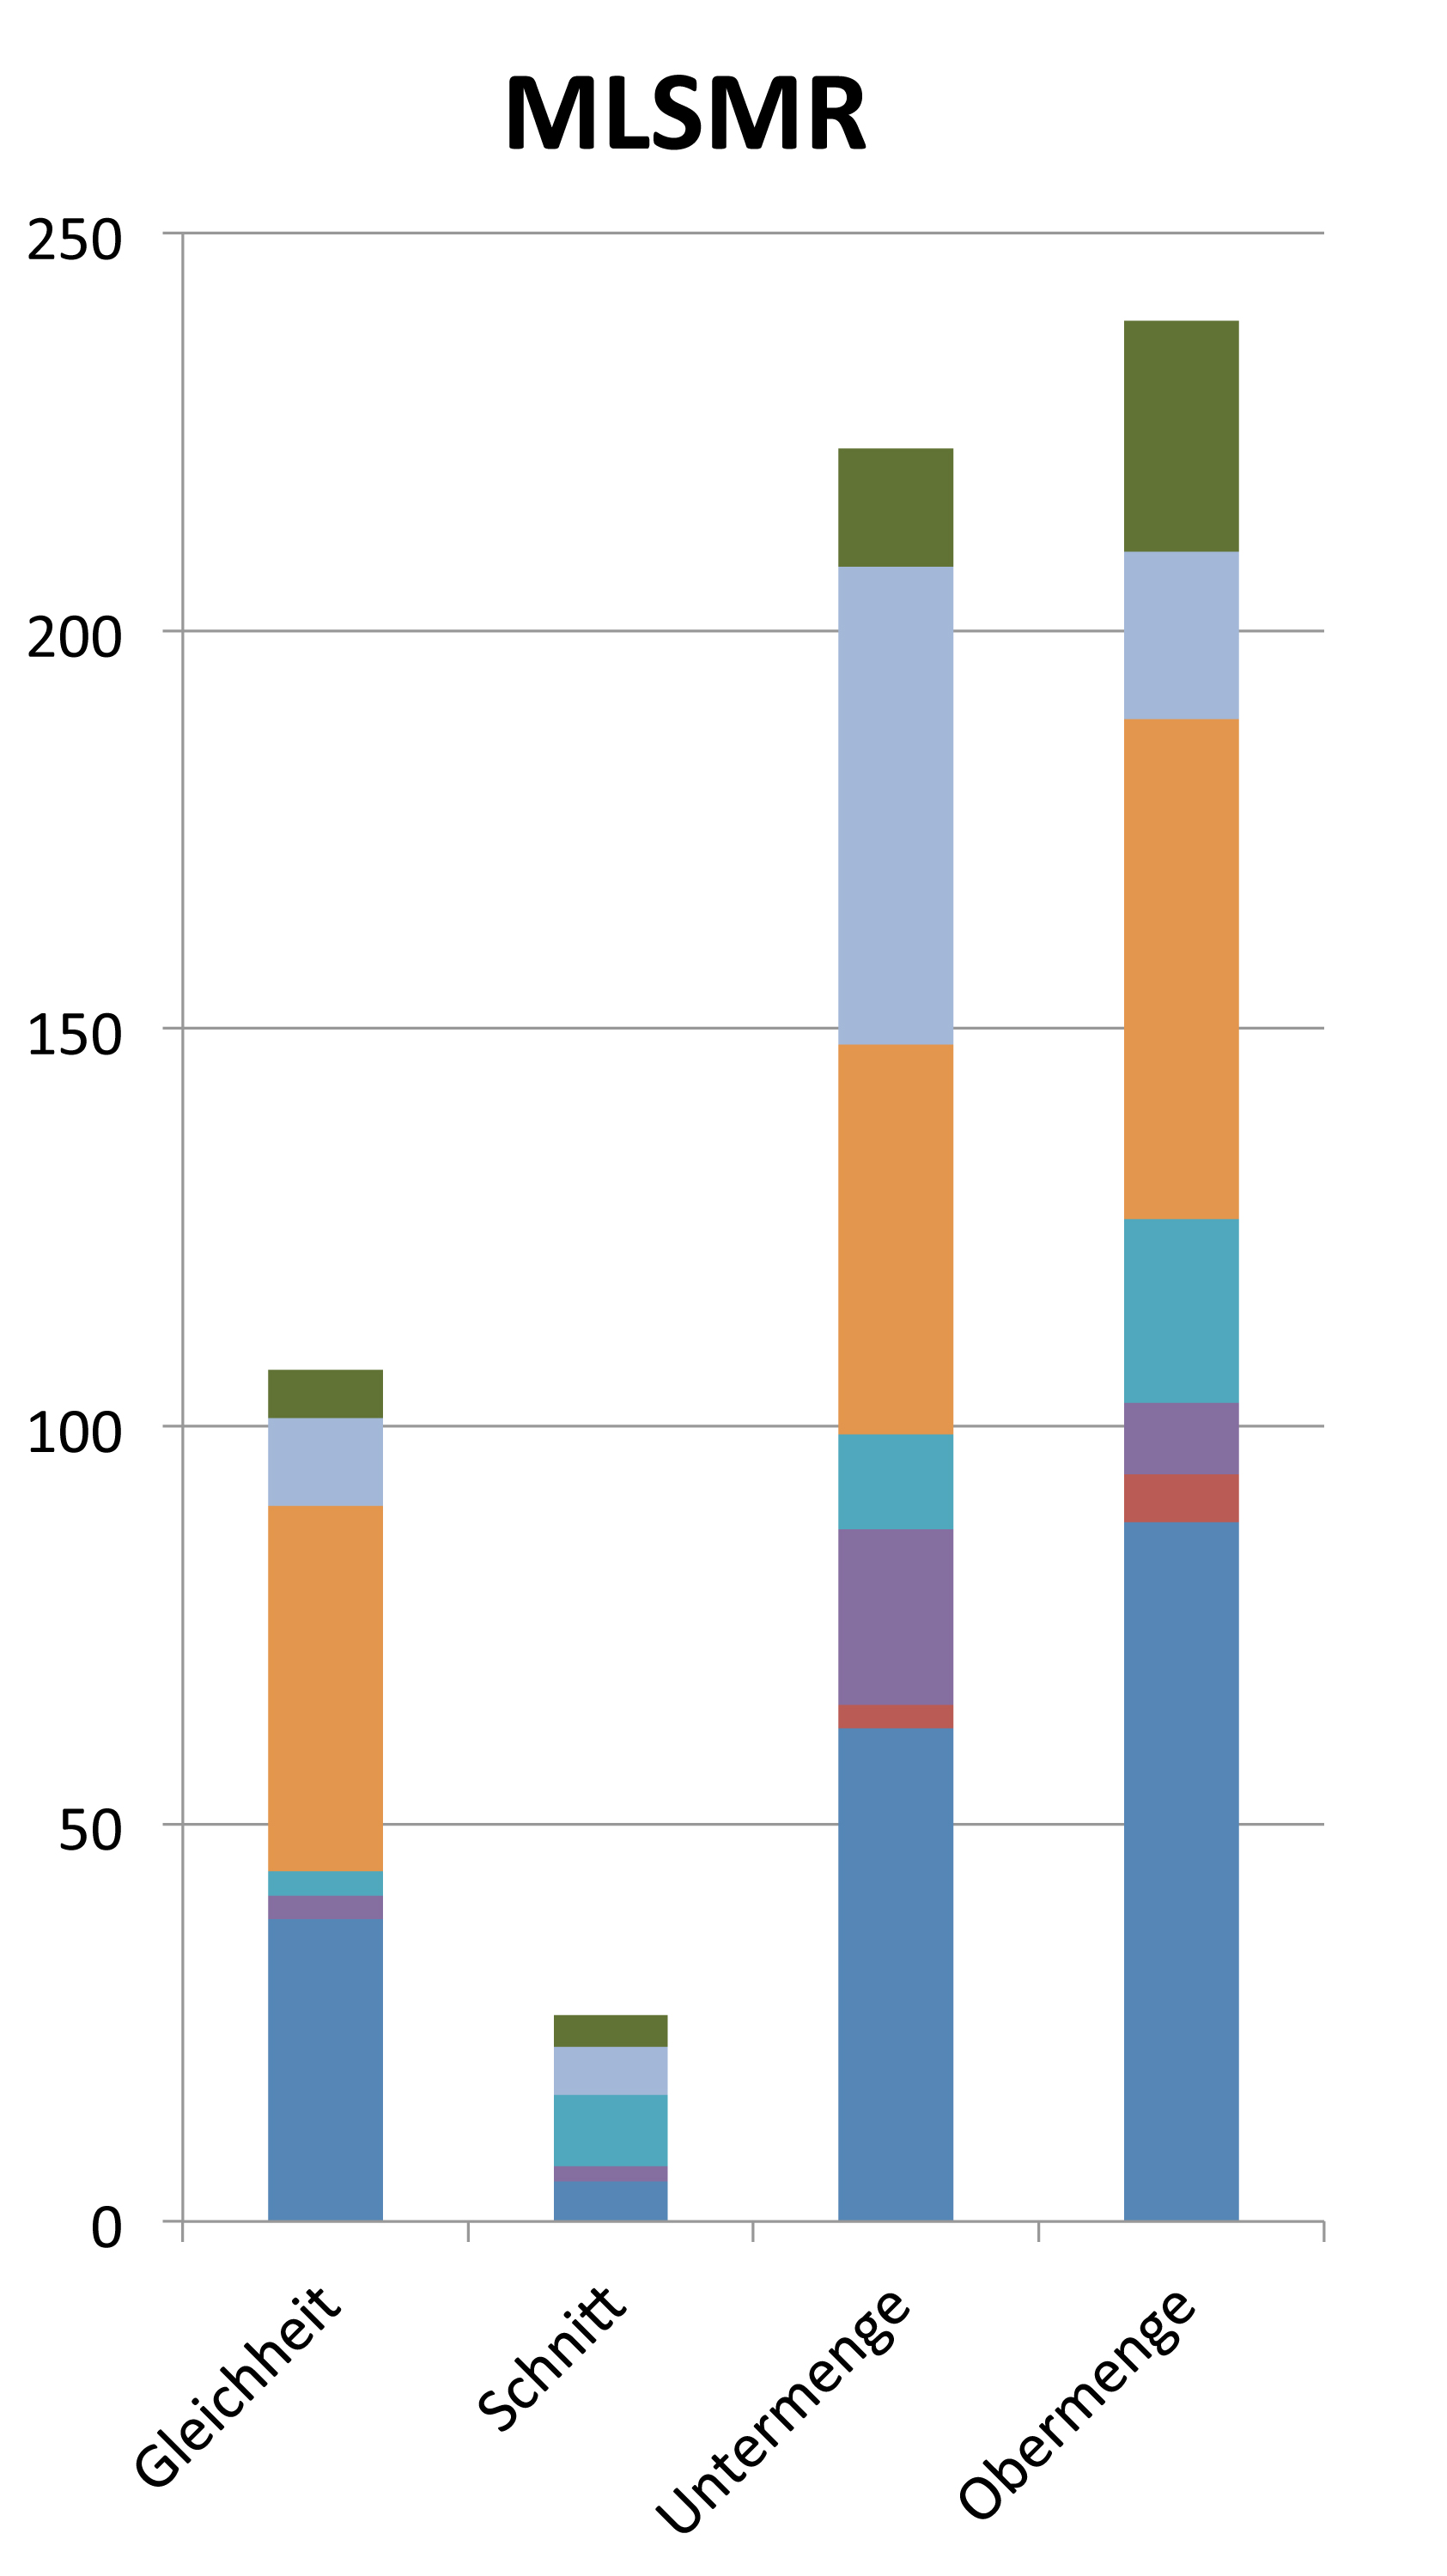
\includegraphics[width=5cm]{images/MLSMR}
		\end{minipage}
		\begin{center}
		\begin{minipage}{7cm}
			\centering
			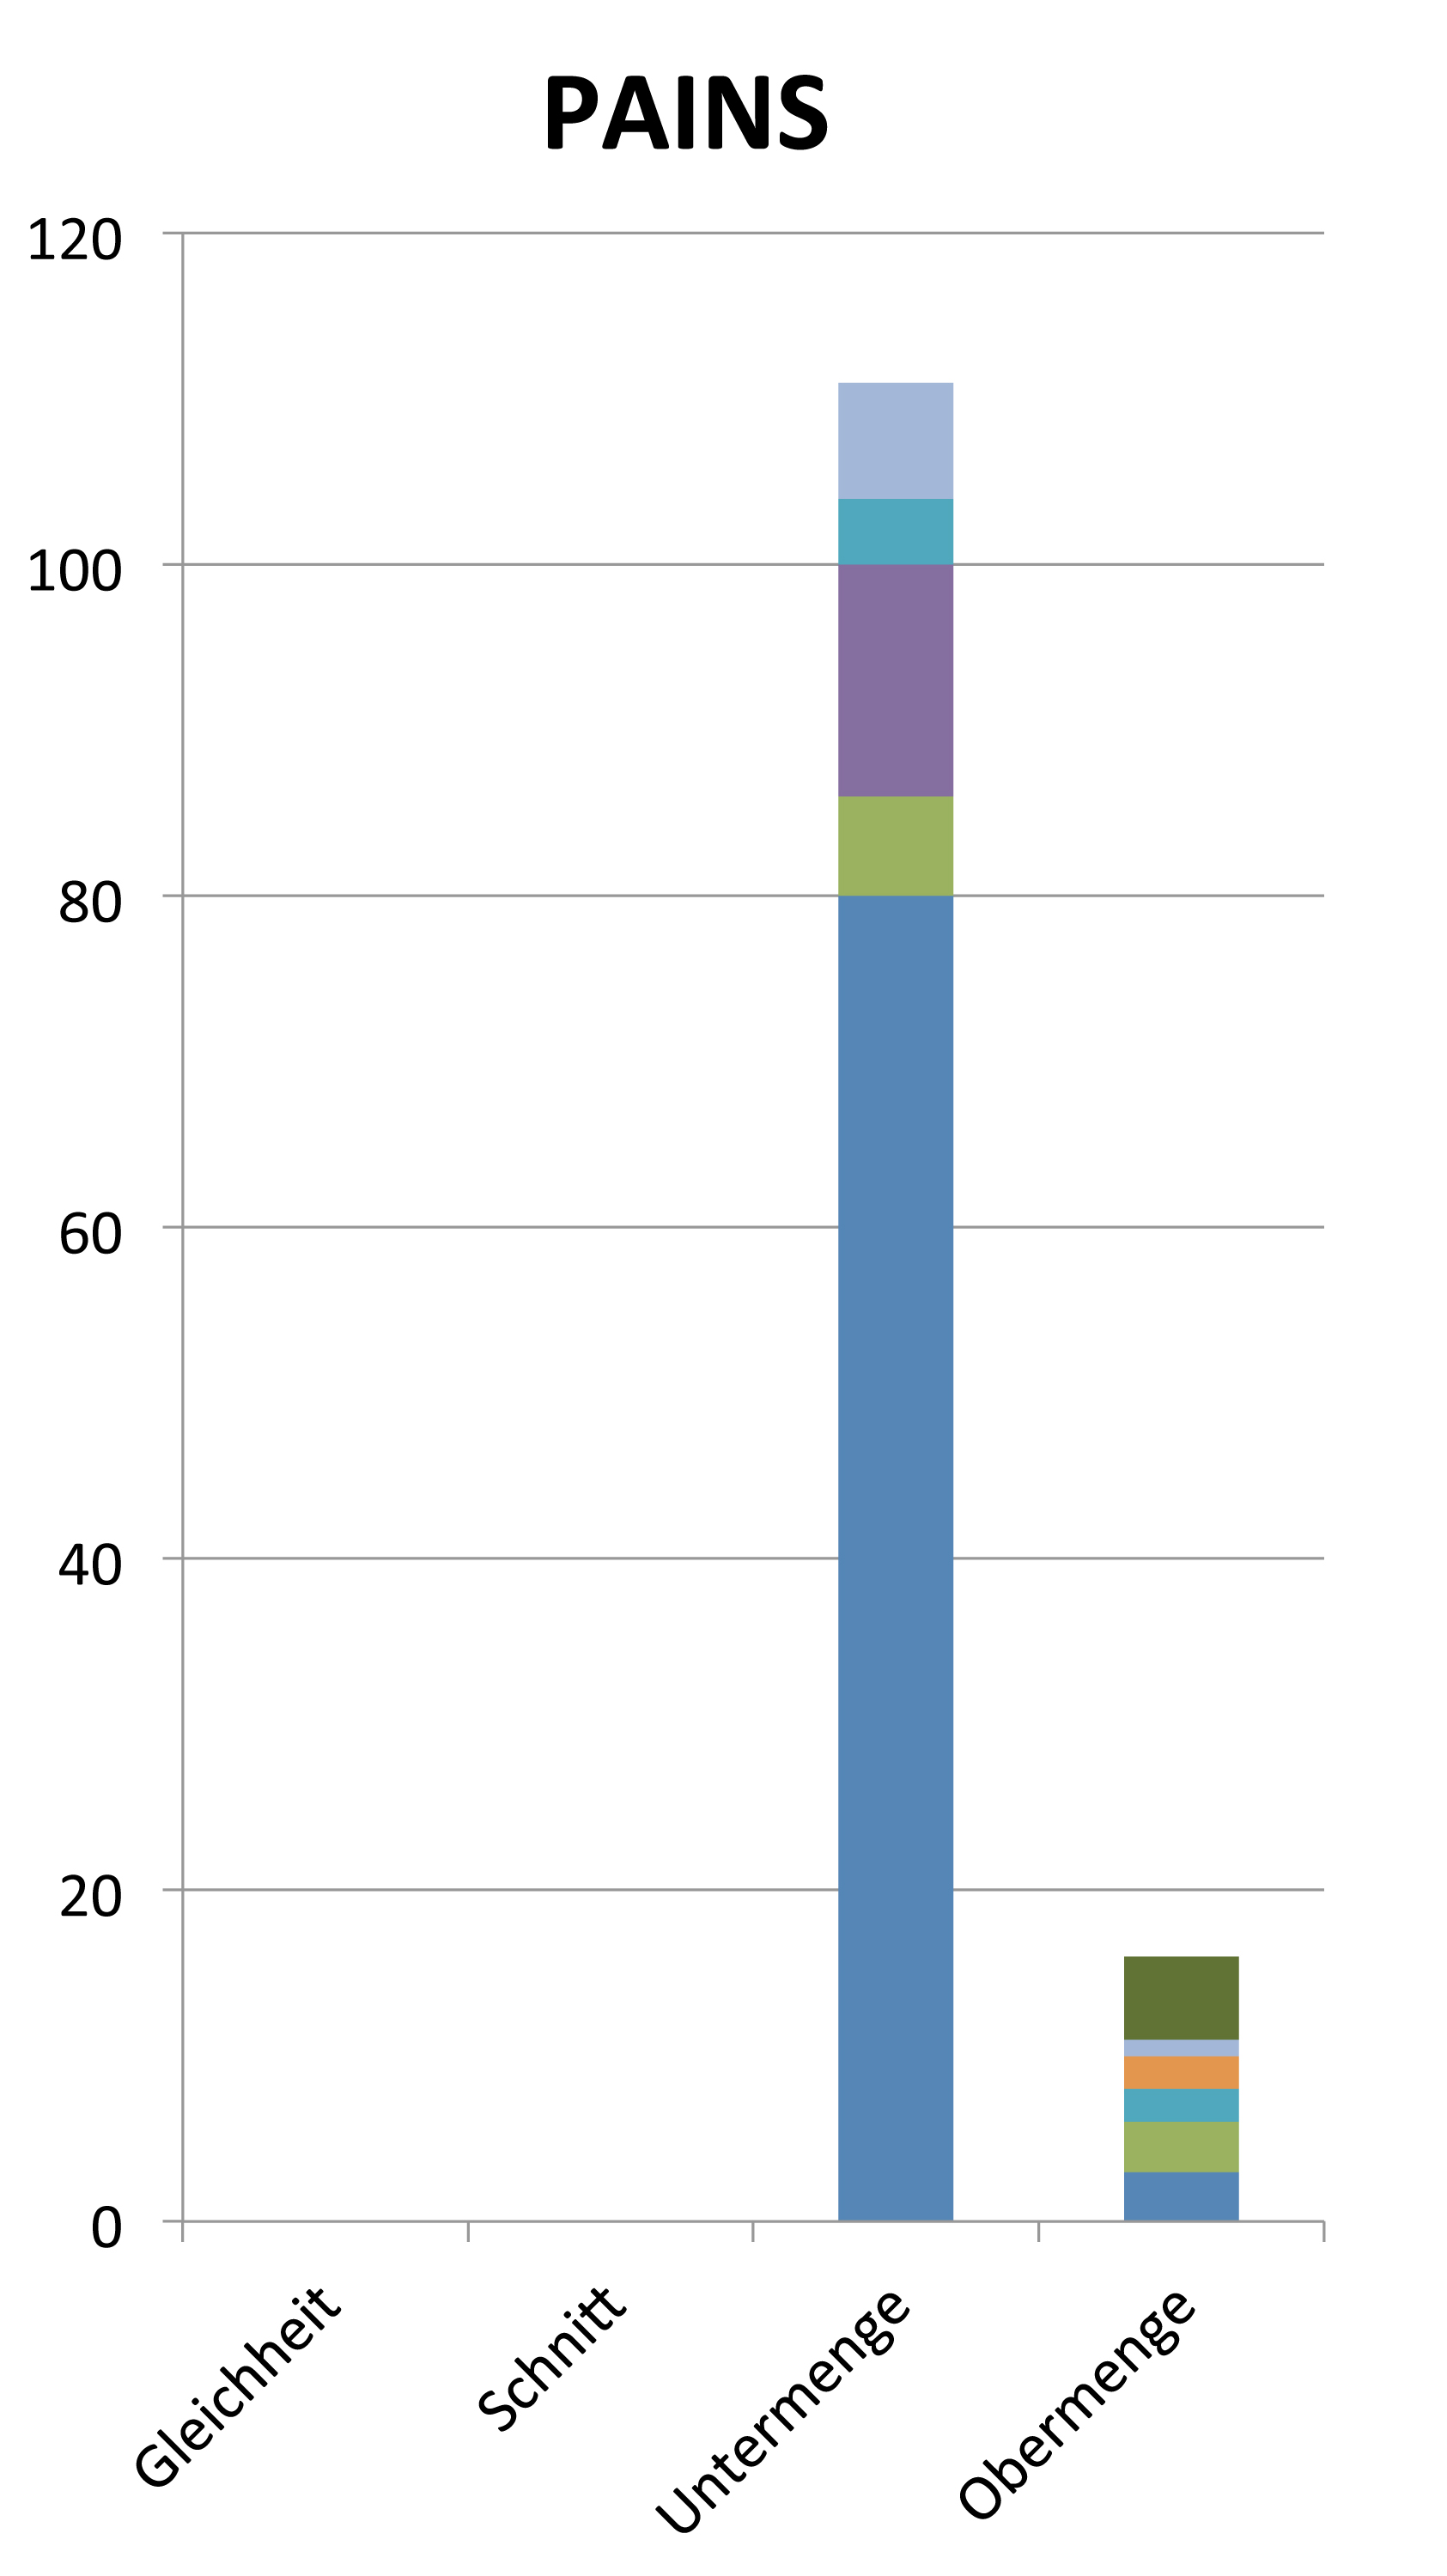
\includegraphics[width=5cm]{images/PAINS}
		\end{minipage}
		\begin{minipage}{7cm}
			\centering
			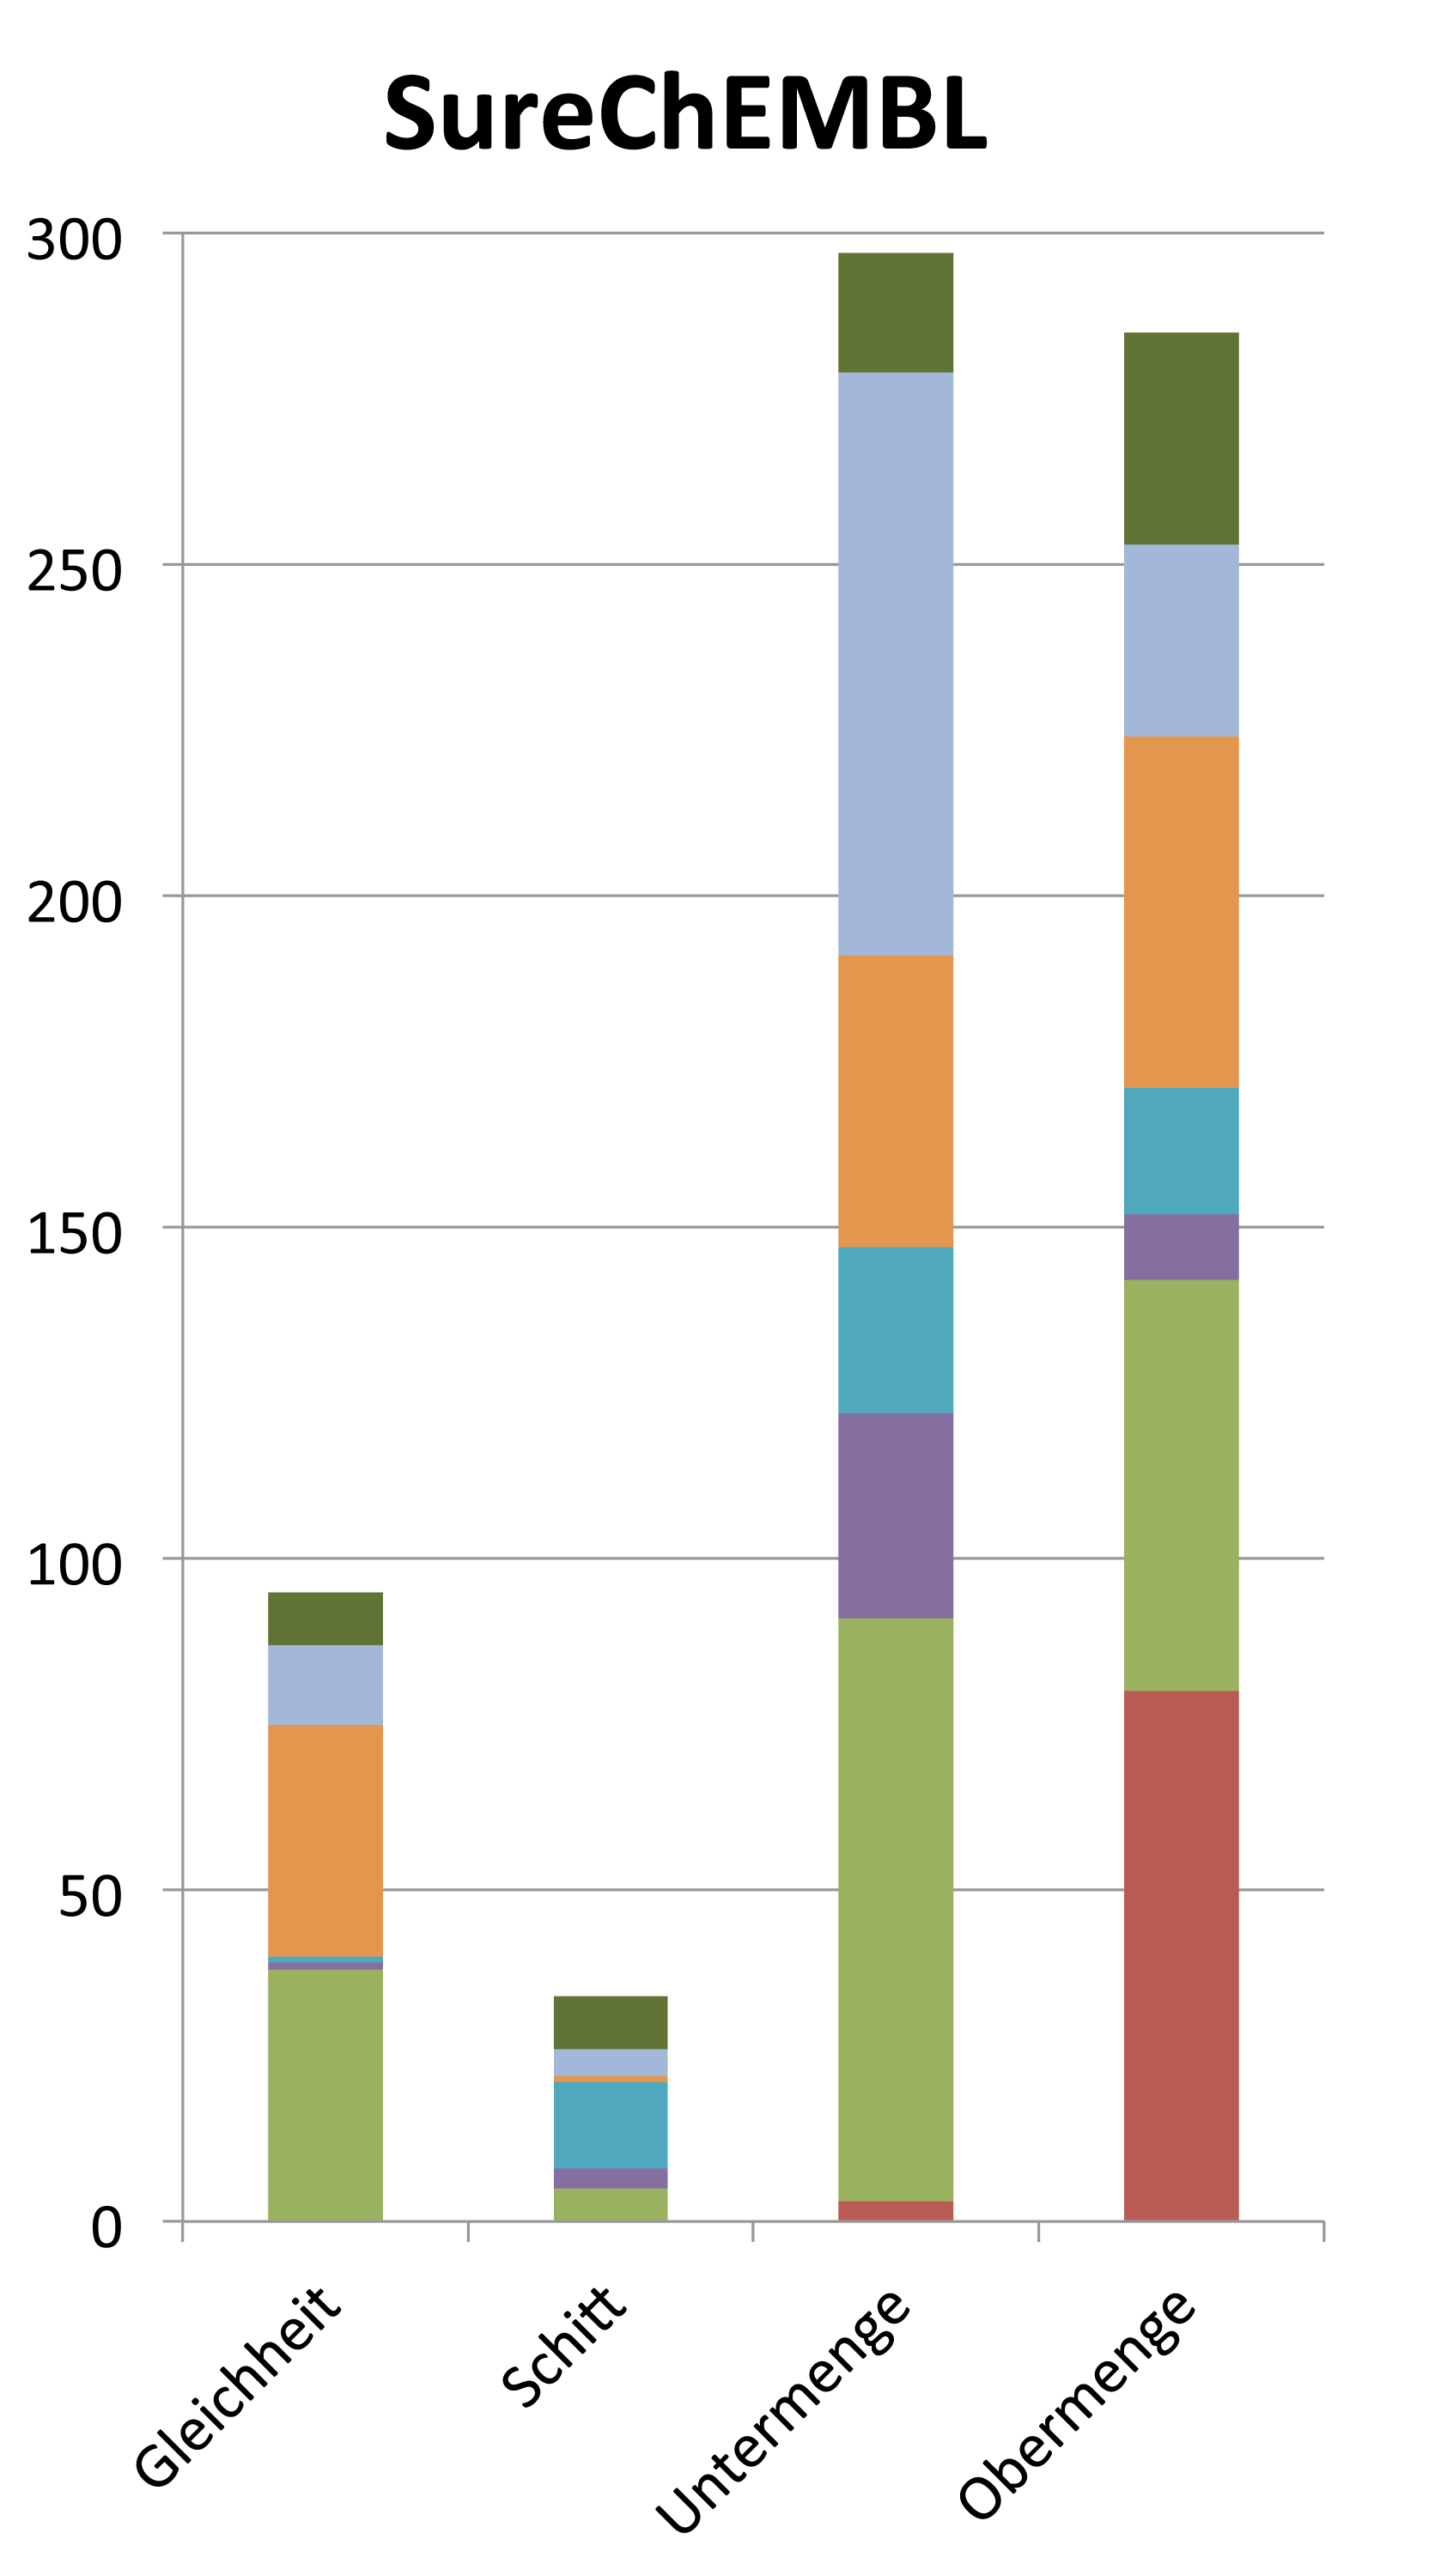
\includegraphics[width=5cm]{images/SureChEMBL}
		\end{minipage}
		\end{center}
	\end{center}
\end{minipage}}
\caption{Zweiter Teil der Experimente: Dargestellt ist f�r wie viele Ziel-SMARTS ein \textit{Mapping} zu den Anfrage-SMARTS der einzelnen SMARTS-Filter (LINT, MLSMR, PAINS, SureChEMBL) gefunden wurde. Die \textit{Mappings} sind Farbig markiert, je nachdem aus welchen anderen Filtern sie stammen. Zu beachten sind die unterschiedlichen Skalierungen (vgl. Tabelle \ref{tab:experiments}).}
\label{abb:experiments2}
\end{figure}
\newpage
\textbf{PAINS} (vgl. Abbildung \ref{abb:experiments2})\\
Die interessantesten Ergebnisse ergaben die Vergleiche mit dem SMARTS-Filter PAINS. Es wurden weder Gleichheits-\textit{Mappings} noch Schnitt-\textit{Mappings} festgestellt, obwohl der Filter mehr als 400 SMARTS-Ausdr�cke nutzt. Auch die geringe Anzahl der Ziel-SMARTS f�r die ein \textit{Mapping} festgestellt wurde weist darauf hin, dass der SMARTS-Filter PAINS nur im geringen Ma�e mit den anderen vergleichbar ist. Es wurden haupts�chlich Unter-\\mengen-\textit{Mappings} gefunden, was darauf schlie�en l�sst, dass die SMARTS-Ausdr�cke eher spezifisch sind. Diese Spezifizierung ist durch eine Konvertierung von SLN-Beschreibungen (\textit{SYBYL line notation} \cite{sln}) in SMARTS-Ausdr�cke entstanden. Dabei wurden die Wasserstoffatome, die in SMARTS-Ausdr�cken als Eigenschaft behandelt werden als Atome �berf�hrt. \cite{painssln}

\textbf{SureChEMBL} (vgl. Abbildung \ref{abb:experiments2})\\
Es wurde bei dem vorgehenden Vergleich auf redundante ein gleicher SMARTS-Ausdruck in der Liste festgestellt. SureChEMBL nutzt einen Filter, der ausgewogen Unter- und Obermengen-\textit{Mappings} aufweist. Dabei ist dieser SMARTS-Filter derjenige der dem Filter PAINS am �hnlichsten ist. SureChEMBL nutzt mit 148 SMARTS-Ausdr�cken einen eher gro�en Filter, der dennoch in ungef�hr gleichen Teilen eine Untermenge sowie eine Obermenge der anderen Filter darstellt. Dadurch l�sst sich sagen, dass SureChEMBL einen SMARTS-Filter nutzt, der ein breites Spektrum von SMARTS-Ausdr�cken nutzt.

\textbf{Zusammenfassung}\\
Abschlie�end l�sst sich sagen, dass mit Hilfe des entwickelten Verfahrens R�ckschl�sse auf die Art der genutzten Filter gezogen werden k�nnen. So Weisen die Filter Glaxo, MLSMR und SureChEMBL eine gro�e �hnlichkeit zueinander auf. Bei anderen Sets wie LINT und Dundee wurde vor allem die Untermenge als h�ufigste Relation festgestellt, was darauf hinweist, dass diese Sets Molek�le im Vergleich grob herausfiltern. BMS und Inpharmatica hingegen, f�r die vor allem \textit{Mappings} gefunden wurden, die zu einer Obermenge geh�ren weisen darauf hin, dass Molek�leigenschaften im Vergleich zu anderen Sets spezifizierter beschrieben sind, und somit weniger Molek�le herausgefiltert werden. PAINS l�sst sich kaum mit den anderen Filtern vergleichen, was auf die Konvertierung von SLNs zur SMARTS zur�ckzuf�hren ist. Filter, die ausgewogen Unter- und Obermengen-\textit{Mappings} zu anderen Filtern besitzen, scheinen gute Repr�sentanten der Filter zu sein. Festgestellt wurde, dass Filter mit einer gro�en Menge an SMARTS-Ausdr�cken, h�ufig auch spezifiziertere SMARTS-Ausdr�cke nutzen. Bis aus der Filter PAINS weisen alle Filter eine hohe �hnlichkeit zueinander auf. Abbildung \ref{abb:experimentsbsp} zeigt f�r alle Filter (au�er PAINS) ein Muster, welches in einer �hnlichen Form in allen Filtern zu finden ist und verdeutlicht die Unterschiede der Filter.

\begin{figure}[h!]
	\begin{minipage}{7cm}
	\begin{tabular}{m{0.18\textwidth} m{0.3\textwidth} m{0.01\textwidth} m{0.1\textwidth}}
		\textbf{BMS: } &\texttt{S(=O)(=O)C\#N} & $\Leftrightarrow$ & 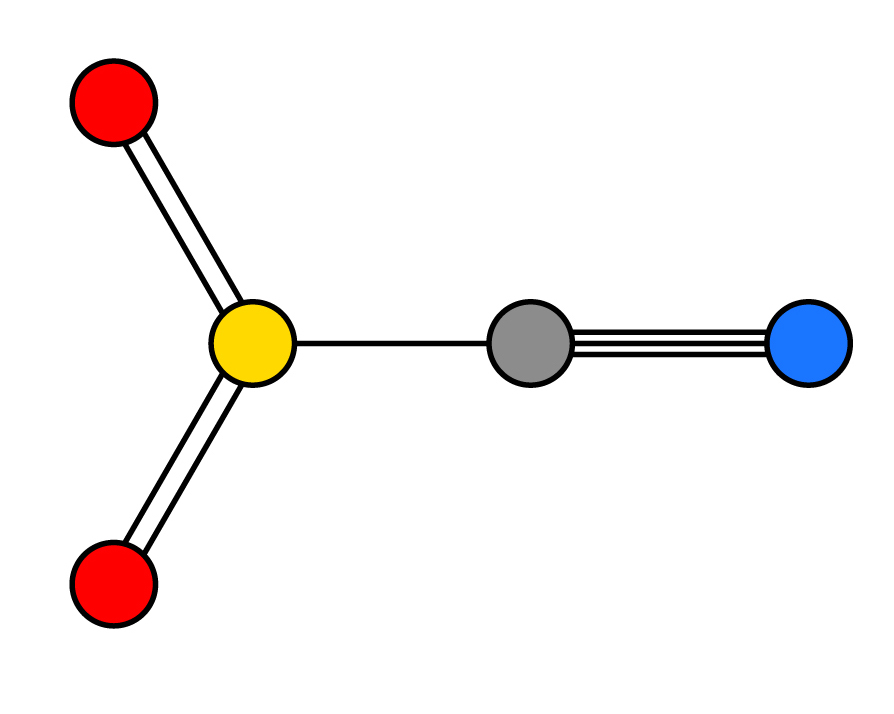
\includegraphics[width=2.2cm]{images/smartsbms}\\
		\textbf{Dundee: } & \texttt{[N,O,S]C\#N} & $\Leftrightarrow$ & 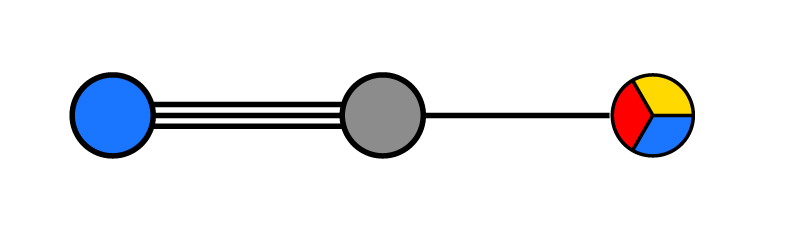
\includegraphics[width=2cm]{images/smartsdundee}\\
		\textbf{Glaxo: } & \texttt{SC\#N} & $\Leftrightarrow$ & 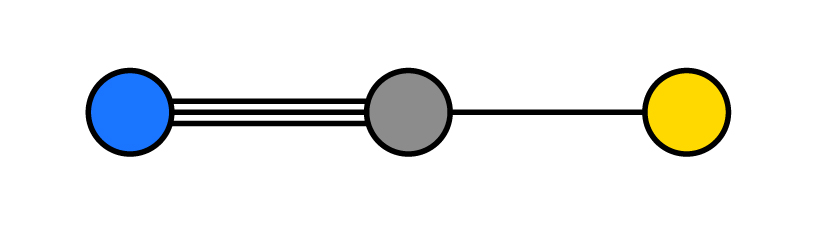
\includegraphics[width=2cm]{images/smartsglaxo}
	\end{tabular}
	\end{minipage}
	\begin{minipage}{8.5cm}
	\centering
	\begin{tabular}{m{0.35\textwidth} m{0.2\textwidth} m{0.01\textwidth} m{0.1\textwidth}}
		\textbf{Inpharmatica: } & \texttt{[O,S]C\#N} & $\Leftrightarrow$ & 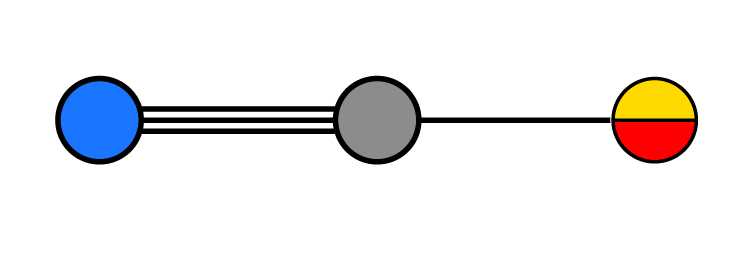
\includegraphics[width=2cm]{images/smartsinphar}\\
		\textbf{LINT: } & \texttt{S-C\#N} & $\Leftrightarrow$ & 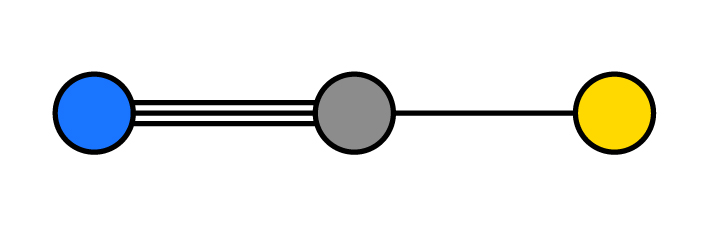
\includegraphics[width=2cm]{images/smartslint}\\
		\textbf{MLSMR: } & \texttt{SC\#N} & $\Leftrightarrow$ & 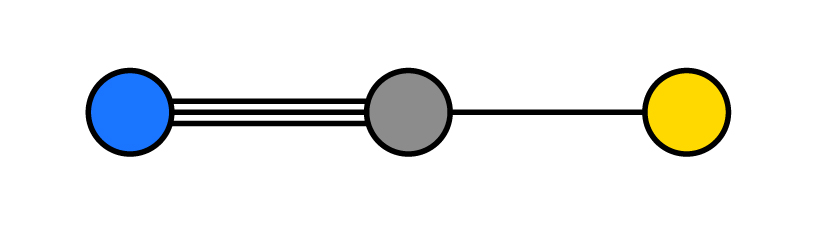
\includegraphics[width=2cm]{images/smartsglaxo}\\
		\textbf{SureChEMBL: } & \texttt{SC\#N} & $\Leftrightarrow$ & 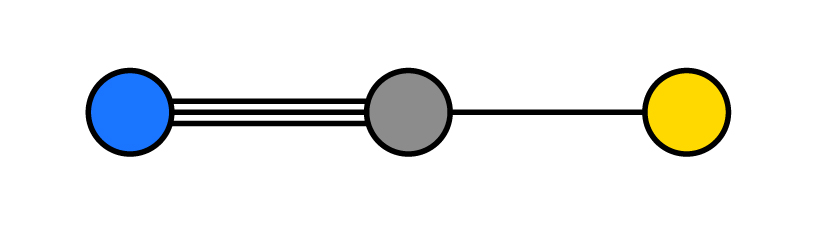
\includegraphics[width=2cm]{images/smartsglaxo}
	\end{tabular}
	\end{minipage}
	\caption{Beispiel eines Musters, welches in allgemeiner oder spezifizierten Form in den Filtern BMS, Dundee, Glaxo, Inpharmatica, LINT, MLSMR und SureChEMBL vorkommt.}
	\label{abb:experimentsbsp}
\end{figure}
%
% EOF
%
%
% Diskussion und Bewertung
%
\section{Fazit}
Das in dieser Arbeit vorgestellte und implementierte Verfahren erm�glicht eine L�sung des in Kapitel \ref{sssec:einleitung} beschriebene Problems. Mit dem entwickelten Verfahren ist es m�glich chemische Muster zu vergleichen.\\
Die bereits bestehenden Konzepte \cite{Master} konnten im Rahmen dieser Arbeit erweitert und verbessert werden.
So wurde die Untersuchung zweier Muster auf eine Schnitt-Relation neu entwickelt und implementiert. Das SMARTS-Atomprimitiv \texttt{h<n>} wurde mit der expliziten Beschreibung (\texttt{H<n>}) zusammengef�hrt, sodass kein zus�tzlicher Aufwand im Verfahren n�tig ist und das Atomprimitiv dennoch verarbeitet werden kann.\\
Die Experimente (vgl. Kapitel \ref{sec:experimente}), die mit Hilfe des entwickelten Verfahrens durchgef�hrt wurden, zeigen eine m�gliche Anwendung der implementierten Methode. Die Ergebnisse erm�glichen es R�ckschl�sse auf die Art und Spezifizierung der SMARTS-Ausdr�cke zu ziehen.

\subsection{Ungel�ste Probleme}\label{ssec:probleme}
Einige SMARTS-Atomprimitve k�nnen von dem vorgestellten Verfahren nicht behandelt werden. Dies verhindert, dass alle SMARTS-Ausdr�cke auf Teilmengen-Relationen �berpr�ft werden k�nnen.\\
Momentan werden bei der �bergabe an das implementierte Verfahren die SMARTS-Ausdr�cke �berpr�ft und gegebenenfalls aussortiert. Aussortiert werden SMARTS-Aus-\\dr�cke, die eine der folgenden Eigenschaften beinhalten:
\begin{itemize}
	\item[] \texttt{@@} oder \texttt{@}: Chiralit�t an tetraedrischen Kohlenstoffen
	\item[] \texttt{@<c><n>}: Chiralit�tsklasse \textless c\textgreater, Chiralit�t \textless n\textgreater 
	\item[] \texttt{@<c><n>?}: Chiralit�tsklasse \textless c\textgreater, Chiralit�t \textless n\textgreater oder nicht spezifiziert
	\item[] \texttt{\$(SMARTSExp)}: Rekursive Ausdr�cke
\end{itemize}
Die drei Eigenschaften betreffend der Chiralit�t sind deshalb problematisch, da sie abh�ng\-ig von den impliziten Eigenschaften sind, die aus der Molek�lgraphenstruktur resultieren.

Ein besonderer Problemfall betrifft die rekursiven Ausdr�cke (siehe Kapitel \ref{sssec:smarts}) der SMARTS-Sprache. Die Einbeziehung einer Umgebung f�r ein Atom oder eine Bindung ist f�r das hier vorgestellte Konzept der Fingerprints als Grundlage der Vergleiche nicht m�glich. Die Eigenschaft ist f�r SMARTS-Ausdr�cke extrem relevant, da sie es erm�glicht mit einer Definition der Umgebung ein chemisches Muster genauer und effizient zu beschreiben.

Es besteht das Problem, dass ein Abgleich der Atommasse durch die Fingerprintgenerierung nicht m�glich ist. Die Atommasse-Eigenschaft, die in den Valenzzust�nden beinhaltet ist, beschreibt lediglich die Masse der Elemente in ihrer nat�rlichen Form. Gewichtsangaben von Isotopen liegen in dem genutzten Konzept der Valenzzust�nde nicht vor.

Ein Problem, welches unabh�ngig von der SMARTS-Sprache ist, betrifft die Schnitt-Relation. Wie in Formel \eqref{eq:fall2} beschrieben gilt entweder f�r Knoten oder Kanten, dass es eine Unter- und eine Obermengenrelation in einem m�glichen \textit{Mapping} gibt.
Formel \eqref{eq:fallprob} beschreibt den Fall bei dem kein \textit{Mapping} erkannt wird, da die Schnitt-Relation Knoten und Kanten der Molek�lgraphen unabh�ngig voneinander beschreibt. Beispiel \ref{bsp:fallprob} zeigt den in \eqref{eq:fallprob} beschriebenen Fall.
\begin{align}
\tag{3}
\begin{split}
& \Big(\forall (v_Q,v_T) \in M_{QT}: \big(LA_{v_Q} =,\cap,\subset,\supset LA_{v_T}\big)\\
&\land \forall (e_Q,e_T) \in M_{QT}: \big(LA_{e_Q} =,\cap,\subset,\supset LA_{e_T}\big)\Big)\\
\land &\Big[\Big(\big(\exists (v'_Q,v'_T)\in M_{QT}\backslash \{(v_Q,v_T)\}: (LA_{v'_Q} \subset LA_{v'_T})\big)\\
&\qquad \lor\big(\exists (e'_Q,e'_T)\in M_{QT}\backslash \{(e_Q,e_T)\}: (LA_{e'_Q} \subset LA_{e'_T})\big) \Big)\\
&\land \Big( \big(\exists (v''_Q,v''_T) \in M_{QT}\backslash \{(e_Q,e_T)\}: ( (v''_Q,v''_T)\neq(v'_Q,v'_T) \land LA_{v''_Q} \supset LA_{v''_T})\big)\\
&\qquad \lor \big(\exists (e''_Q,e''_T) \in M_{QT}\backslash \{(e_Q,e_T)\}: ( (e''_Q,e''_T)\neq(e'_Q,e'_T) \land LA_{e''_Q} \supset LA_{e''_T})\big) \Big)\Big]
\end{split}
\label{eq:fallprob} 
\end{align}

\begin{bsp}
	\label{bsp:fallprob}
\end{bsp}
\begin{table}[h]
	\centering
	\begin{tabular}{l | c c c}
		Anfrage-SMARTS & \texttt{[Cl,I]} & $=$ & \texttt{O} \\
		Teilmengen-Relation & $\supset$ & $\subset$ & $=$ \\
		Ziel-SMARTS & \texttt{[Cl]}& $\sim$ & \texttt{O}\\
	\end{tabular}
\end{table}

Ein interessantes Problem, welches durch die Auswertung der Experimente (vgl. Kapitel \ref{sec:experimente}) aufgedeckt wurde, betrifft Ringschl�sse.
Untersucht wurden die SMARTS-Ausdr�cke auf Gleichheit und Schnitt-Relation. Beispiel \ref{bsp:problemring} zeigt das Ergebnis des Programms \textit{SmartsSmarts}. Offensichtlich wurde eine Schnitt-Relation festgestellt, obwohl Gleichheit festgestellt werden sollte.\\

\begin{bsp}
	\label{bsp:problemring}
\end{bsp}
\begin{table}[h]
	\centering
	\begin{tabular}{l l | l}
		\textbf{Schnitt:} & Anfrage-SMARTS & \texttt{[C:1]1[C:2][N,S,O:3]1}\\
		& Ziel-SMARTS & \texttt{[C:1]1[O,S,N:3][C:2]1}\\
		& Anfrage-SMARTS & \texttt{[C:1]1[C:2][N,S,O:3]1}\\
		& Ziel-SMARTS & \texttt{[C:2]1[O,S,N:3][C:1]1}
	\end{tabular}
\end{table}	

\newpage
\section{Weiterf�hrende Arbeit} \label{sec:ausblick}
Das Problem dessen L�sung am interessantesten ist, ist die der Einbeziehung der rekursiven Ausdr�cke. Ein Ansatz w�re es, falls eine Beschreibung eines Anfrage-SMARTS einen rekursiven Ausdruck besitzt, diese als Eigenschaft zu vergleichen. Eine �berpr�fung, ob es im Ziel-SMARTS eine, der Teilmengen-Relation entsprechende, rekursive Beschreibung gibt, w�rde diesen Vergleich realisieren.
Im ersten Schritt w�rde ohne Einbezug der rekursiven Ausdr�cke ein \textit{Mapping} gesucht werden. Falls es rekursive Beschreibungen von Atomen oder Bindungen gibt, w�rde im n�chsten Schritt �berpr�ft werden, ob das entsprechende Atom oder die entsprechende Bindung des Ziel-SMARTS einen rekursiven Ausdruck besitzt, der der Teilmengen-Relation entspricht. Dabei wird f�r Gleichheit und Schnitt-Relation das bestehende Verfahren genutzt. Die zu vergleichenden rekursive Ausdr�cke werden an das Verfahren �bergeben, und gepr�ft, ob es ein \textit{Mapping} gibt. Bei Unter- und Obermenge wird, falls es f�r beide Partner des \textit{Mappings} einen rekursiven Ausdruck gibt, analog vorgegangen. Falls es nur f�r einen \textit{Mapping}-Partner eine rekursiven Beschreibung gibt, gilt:\\
\textbf{Untermenge:} Der \textit{Mapping}-Partner des Anfrage-SMARTS hat eine rekursive Beschreibung.\\
\textbf{Obermenge:} Der \textit{Mapping}-Partner des Ziel-SMARTS hat eine rekursive Beschreibung.

F�r die Probleme bez�glich der nicht beachteten SMARTS-Primitive m�sste ein Konzept entwickelt werden, welches die zu beachtenden Eigenschaften behandeln kann. Ein Ansatz w�re f�r die Chiralit�t die Information als kurze String-Repr�sentation zu speichern und diese zu vergleichen. �hnlich zum Ansatz f�r die rekursiven Ausdr�cke, kann so gegebenenfalls die Eigenschaft abgeglichen werden.

Das Fehlverhalten welches f�r Beispiel \ref{bsp:problemring} festgestellt wurde, konnte bereits eingegrenzt werden. Es wurde keine Gleichheit festgestellt, da f�r die Knoten \texttt{[N,S,O]} und  \texttt{[O,S,N]} keine Gleichheit festgestellt werden konnte. �bergibt man nur diese beiden Knoten an das Programm wird eine Gleichheit festgestellt. Auch wenn die Ringbindung (gekennzeichnet durch das Zahlenpaar "`1"') entfernt wird, wird eine Gleichheit der beiden SMARTS-Ausdr�cke festgestellt. Das Problem liegt also an den beiden Knoten \texttt{[N,S,O]} und  \texttt{[O,S,N]} in Zusammenhang mit einem Ringschluss. Es wurde weiter festgestellt, dass solange die erste logische Alternative in beiden Knoten gleich ist, das Problem nicht auftritt.\\
Das Problem tritt also auf wenn es in beiden SMARTS-Ausdr�cken einen Knoten gibt, mit den gleichen logischen Alternativen. Diese Knoten m�ssen in einem Ring enthalten sein. Zudem muss an der ersten Position der Knoten unterschiedliche logische Alternativen stehen. Bis zu diesem Zeitpunkt konnte noch kein L�sungsansatz entwickelt werden.
%
% EOF
%

% Anhang
% ----------------------------------------------------------------------------------------------------------
\pagenumbering{Roman}
\setcounter{page}{1}
%\lhead{Anhang \thesection}

% Anhang
%\thispagestyle{empty}
\appendix
%\chapter{Anhang}

\section{Software User Guide} \label{userguide}

\subsection{Command Line Syntax} 

Command Line Syntax beginnt immer mit dem Command Line Programmnamen. Dem Programmnamen k�nnen dann Optionen und Dateinamen folgen. Die Optionen k�nnen in beliebiger Reihenfolge, angef�hrt von einem Minus und getrennt mit einem Leerzeichen, angegeben werden.\\

Das folgende Beispiel zeigt die Command Line Syntax, um \textit{SmartsSmarts} mit einer SMARTS Datei auszuf�hren:
\begin{itemize}
	\item
	\begin{itemize}
		\item Richtig: \textbf{\texttt{SmartsSmarts -t  /home/targetSMARTS.txt}}
		\item Falsch: \textbf{\texttt{SmartsSmarts -t/home/targetSMARTS.txt}}
	\end{itemize}
	\item Es m�ssen immer korrekte Dateiendungen mit angegeben werden (z.B.  \texttt{.txt})
\end{itemize}

\subsection{Command Line Options}

Die folgenden Optionen sind in dem \texttt{SmartsSmarts}-Programm beinhaltet:
\begin{itemize}
	\item \texttt{-h} (Hilfe)
	\item \texttt{-s} (Anfrage-SMARTS Input (String))
	\item \texttt{-l} (Anfrage-SMARTS Input (Datei))
	\item \texttt{-t} (Ziel-SMARTS Input)
	\item \texttt{-r} (Teilmengen-Relation)
	\item \texttt{-v} (Validierung (Entwickleroption))
\end{itemize}

\subsubsection*{-h (Hilfe)}
Wenn der Programmname mit dieser Option aufgerufen wird, wird eine Meldung angezeigt, die alle Optionen, exklusive der Entwickleroptionen, zusammen mit ihren ben�tigten Parametern, ihren Datentypen sowie ihren Beschreibungen f�r das Programm auflistet.\\
\textbf{Syntax:}\\
\noindent \hspace*{10mm} \textbf{\texttt{-h}}\\
\noindent \hspace*{10mm}\textbf{\texttt{--help}}

\subsubsection*{-s (Anfrage-SMARTS Input (String))}
Wenn der Programmname mit dieser Option eingeben wird, ist als weiterer Parameter ein String erforderlich, welcher in Form eines SMARTS vorliegt.\\
\textbf{Syntax:}\\
\noindent \hspace*{10mm}\textbf{\texttt{-s }}\textit{"querySMARTS"}\\
\noindent \hspace*{10mm}\textbf{\texttt{--querystring }}\textit{"querySMARTS"}\\

\subsubsection*{-l (Anfrage-SMARTS Input (Datei))}
Wenn der Programmname mit dieser Option eingeben wird, ist als weiterer Parameter ein Name einer Datei erforderlich, welche SMARTS-Strings beinhaltet.\\
\textbf{Syntax:}\\
\noindent \hspace*{10mm}\textbf{\texttt{-l }}\textit{querySMARTS}\\
\noindent \hspace*{10mm}\textbf{\texttt{--querylist }}\textit{querySMARTS}\\
\\ \textbf{Hinweis:}\\
Die SMARTS Input-Datei darf pro Zeile nur einen SMARTS-String beinhalten.

\subsubsection*{-t (Ziel-SMARTS Input)}
Wenn der Programmname mit dieser Option eingeben wird, ist als weiterer Parameter ein Name einer Datei erforderlich, welche SMARTS-Strings beinhaltet.\\
\textbf{Syntax:}\\
\noindent \hspace*{10mm}\textbf{\texttt{-t }}\textit{targetSMARTS}\\
\noindent \hspace*{10mm}\textbf{\texttt{--target }}\textit{targetSMARTS}\\
\\ \textbf{Hinweis:}\\
Die SMARTS Input-Datei darf pro Zeile nur einen SMARTS-String beinhalten.

\subsubsection*{-r (Teilmengen-Relation)}
Wenn der Programmname mit dieser Option eingeben wird, ist als weiterer Parameter ein String erforderlich, welcher in Form eines vier-elementigen Bitstrings f�r Schnitt-Relation vorliegt.\\
\textbf{Syntax:}\\
\noindent \hspace*{10mm}\textbf{\texttt{-r }}\textit{"Bitstring"}\\
\noindent \hspace*{10mm}\textbf{\texttt{--relationship }}\textit{"Bitstring"}

\textbf{Hinweis:}\\
Der Bitstring muss folgende Syntax einhalten:
\begin{itemize}
	\setlength\itemsep{0em}\setlength\parskip{0em}
	\item Der Bitstring besteht aus 4 Zeichen
	\item Erlaubte Zeichen sind "`0"' und "`1"'
	\item Mindestens ein Zeichen muss eine "`1"' sein
	\item Dabei sind die Teilmengen-Relationen folgenden Bits zugeordnet:
	\begin{itemize}
		\setlength\itemsep{0em}\setlength\parskip{0em}
		\item 1. Bit: Gleichheit \hspace{0.5cm}(\texttt{1000})
		\item 2. Bit: Schnitt \hspace{1.04cm}(\texttt{0100})
		\item 3. Bit: Untermenge \hspace{0.168cm}(\texttt{0010})
		\item 4. Bit: Obermenge \hspace{0.29cm}(\texttt{0001})
	\end{itemize}
\end{itemize}

\subsubsection*{-v (Validierung (Entwickleroption))}
Wenn der Programmname mit dieser Option eingeben wird, ist als weiterer Parameter ein Dateiname erforderlich, welche Molek�lbeschreibungen beinhaltet. M�gliche Dateiformate sind:  \texttt{.mol2}, \texttt{.pdb}, \texttt{.sdf}, \texttt{.smi}, \texttt{.smiles}\\
Die Optionen \texttt{-s} (oder \texttt{-l}), \texttt{-t} und  \texttt{-r} sind bei dieser Option erforderlich.
Es handelt sich bei dieser Option um eine Entwickleroption, mit der die Validierung des Programms ausgef�hrt wird.\\
\textbf{Syntax:}\\
\noindent \hspace*{10mm}\textbf{\texttt{-v }}\textit{molecules}\\
\noindent \hspace*{10mm}\textbf{\texttt{--validation}} \textit{molecules}

Beim Aufruf des Programmes m�ssen die Optionen \texttt{-s} (oder \texttt{-l}), \texttt{-t} und  \texttt{-r} immer mit angegeben werden.
\pagebreak
\section{Softwarearchitektur}\label{sec:softwarearch}
\begin{figure}[h!]
	\centering
	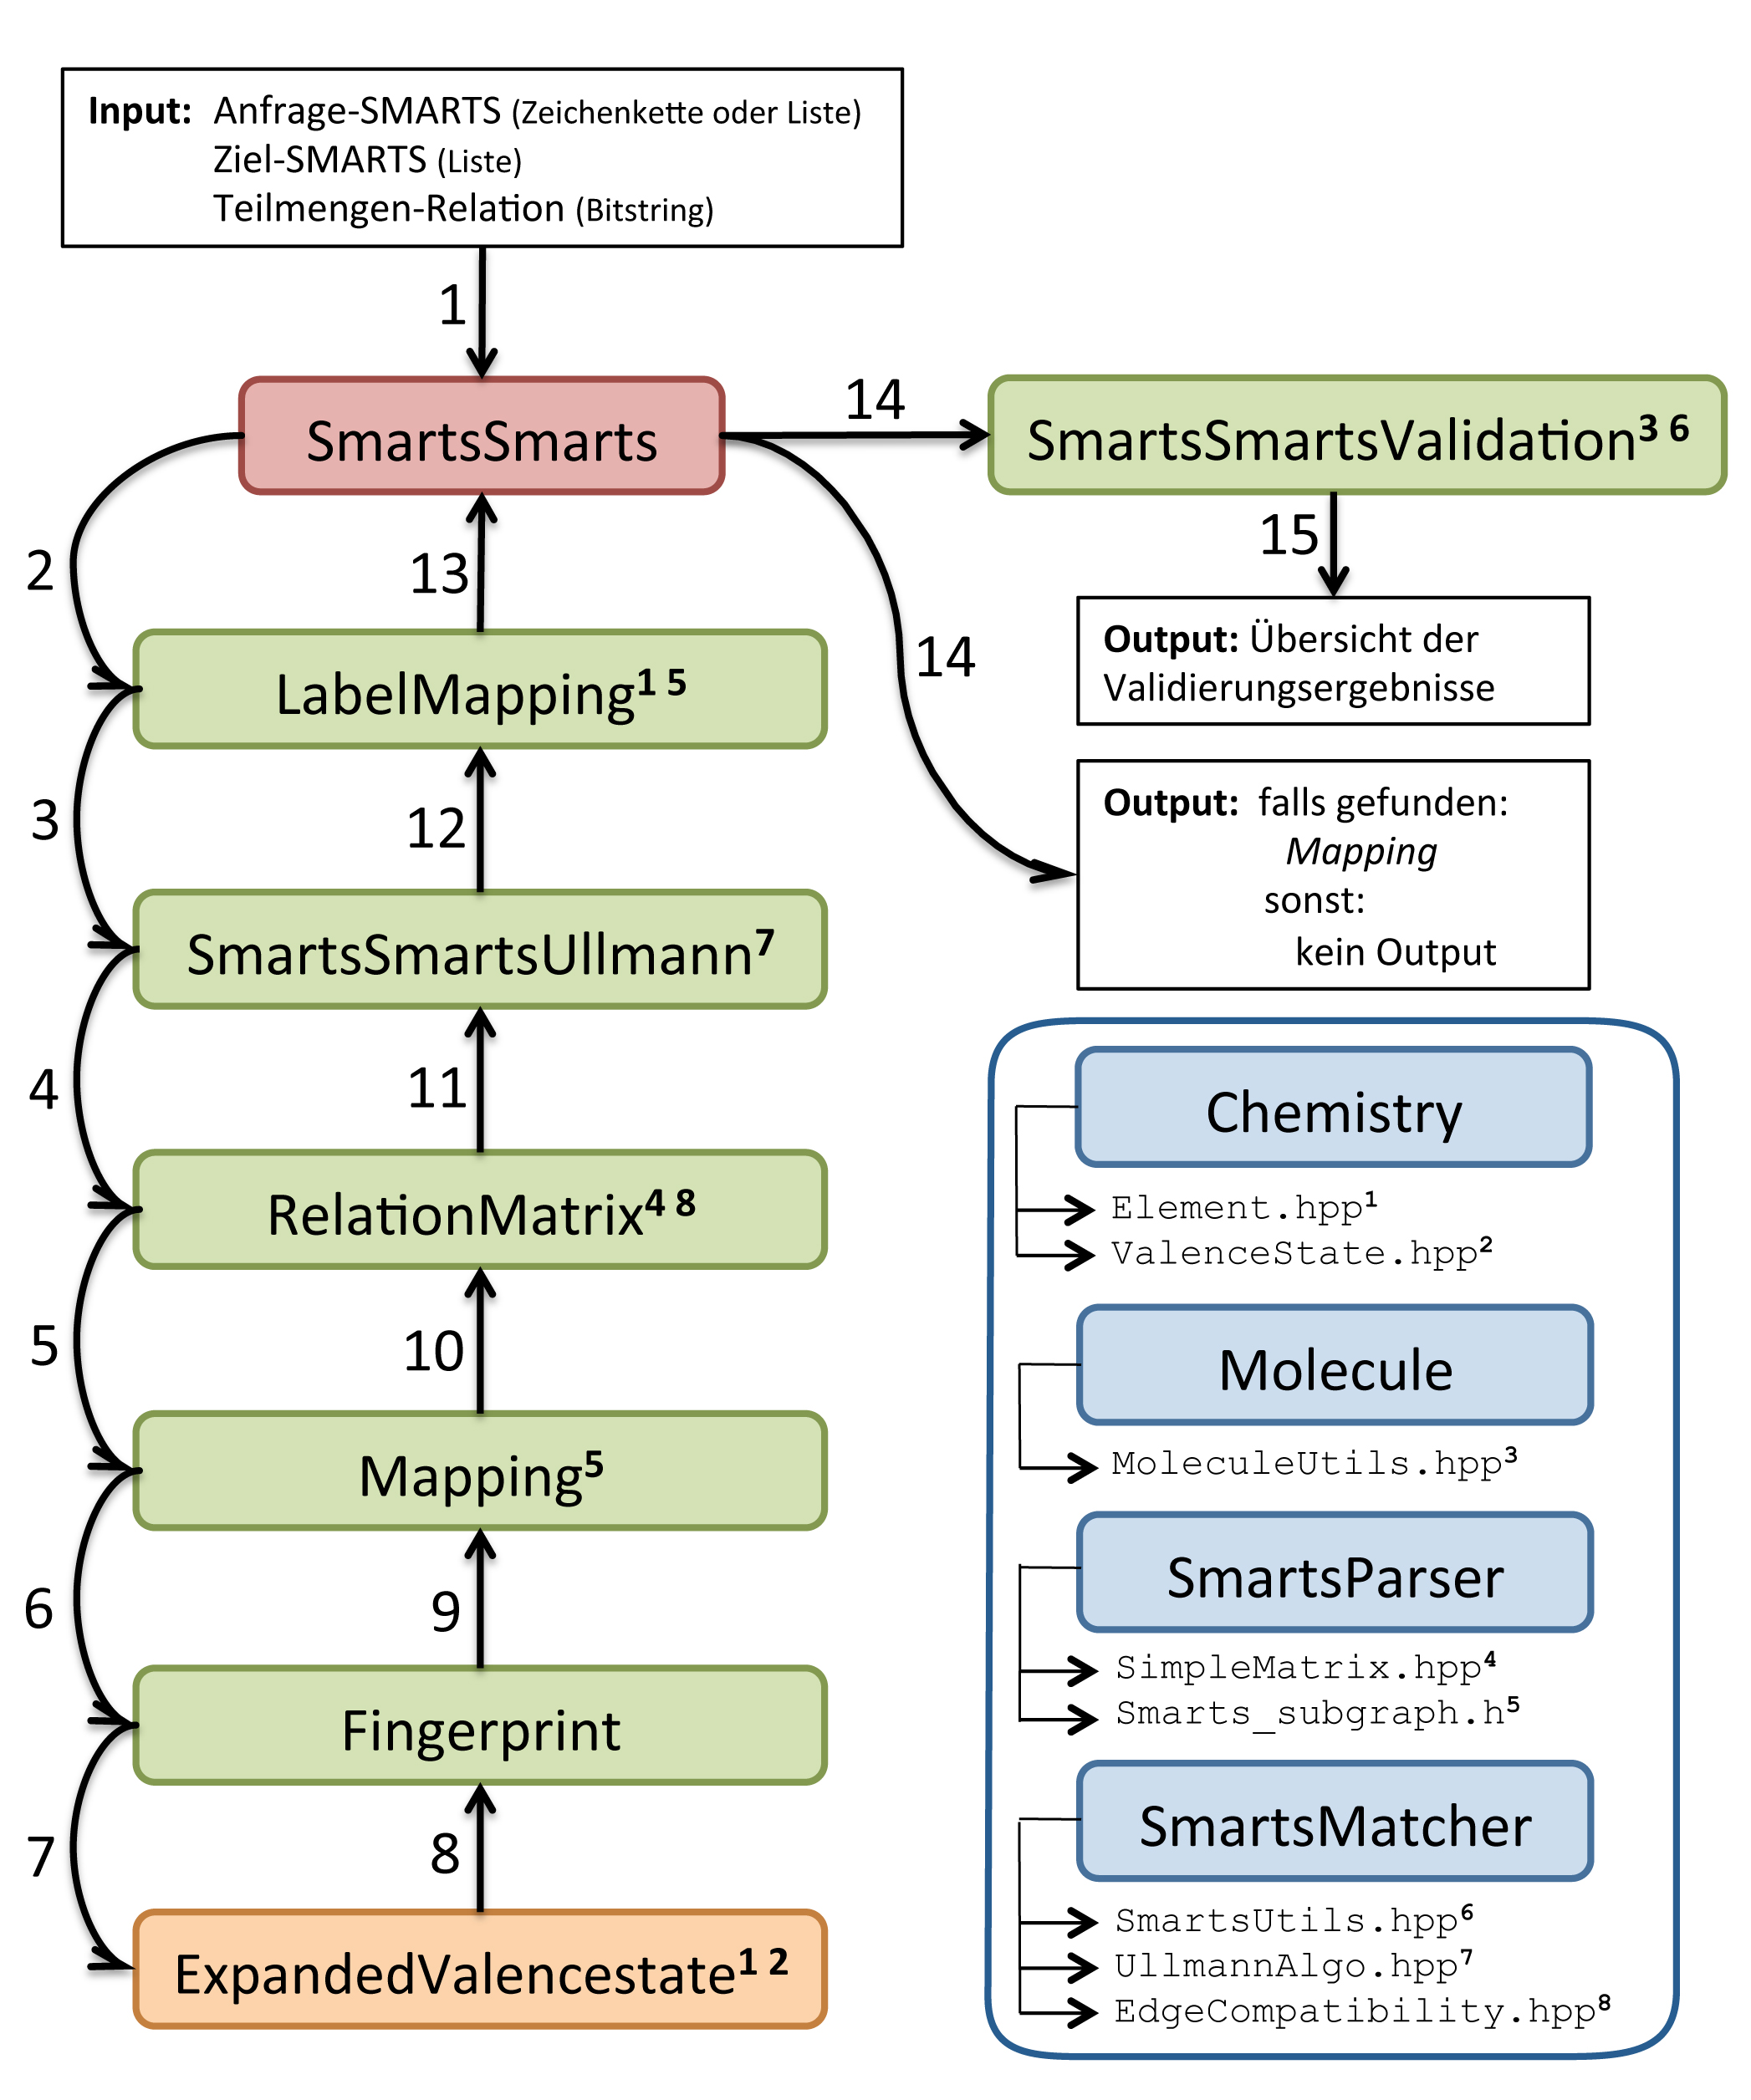
\includegraphics[width=14cm]{images/software}
	\caption{Schematische Darstellung der Softwarestruktur des Programms \textit{SmartsSmarts}}
	\label{fig:softwarestruk}
\end{figure}
\vspace{3mm}

In Abbildung \ref{fig:softwarestruk} ist die Softwarestruktur des Programms \textit{SmartSmarts} (rot) schematisch dargestellt. Ausgehend von den Eingabedateien (Input) wird durch die nummerierten Pfeile der Ablauf des Programms dargestellt. Es wird gezeigt, welche Module (gr�n) und Klassen (orange) des Programms sich gegenseitig nutzen. Welche Module aus der NAOMI-Softwarebibliothek (blau) an welchen Stellen des \textit{SmartsSmarts} Programms genutzt werden, ist durch Hochzahlen gekennzeichnet. Im folgenden Kapitel werden die wichtigsten Module und Klassen erl�utert.

\newpage
\section{Wichtige Module und Klassen}

\textbf{\large LabelMapping.hpp}
\begin{align*}
\hspace{0.3cm}\texttt{std::pair<std::string,std::string>} & \texttt{addLabels(const std::string \&smarts\_q,}\\
& \texttt{const std::string \&smarts\_t,}\\
& \texttt{const std::vector<std::vector<int>>}\\
& \qquad \texttt{existingLabels)}
\end{align*}
Diese Funktion versieht anhand von Anfrage-SMARTS, Ziel-SMARTS und einer Liste �ber die bestehenden \textit{Label} beide SMARTS-Ausdr�cke mit \textit{Labeln} zur eindeutigen Kennzeichnung und gibt diese zur�ck.
\begin{align*}
	\hspace{0.3cm}\texttt{std::pair<std::string,}&\texttt{std::string> recalculateLabels(const std::string}\\
	& \texttt{ \&smarts\_q, const std::string \&smarts\_t,}\\
	& \texttt{ const std::vector<std::vector<int>>\&existingLabels,}\\
	& \texttt{ const Base::SimpleMatrix<int>\&solutions)}
\end{align*}
	Diese Funktion bekommt Anfrage-SMARTS, Ziel-SMARTS, eine Liste �ber die bestehenden \textit{Label} und eine Permutationsmatrix, die einen Isomorphismus repr�sentiert, �bergeben. Sie setzt die \textit{Label} anhand der gefundenen L�sung neu und gibt Anfrage- und Ziel-SMARTS zur�ck.\\

\textbf{\large SmartsSmartsUllmann.hpp}
\begin{flalign*}
\hspace{0.3cm}\texttt{std::vector<Base::SimpleMatrix<int>>} &\texttt{ getUllmannSolutions}&\\
&\qquad \texttt{(const std::string \&smarts\_q,}&\\
&\qquad \texttt{ const std::string \&smarts\_t,}&\\
&\qquad \texttt{ const std::string \&relation)}&
\end{flalign*}
Diese Funktion berechnet mit einem Anfrage-SMARTS, Ziel-SMARTS und einer Teilmengen-Relation in Form eines Bitstrings ein eindeutiges \textit{Mapping} und gibt dieses als Permutationsmatrix zur�ck.\\

\textbf{\large RelationMatrix.hpp}
\begin{flalign*}
\hspace{0.3cm}\texttt{Base::SimpleMatrix<int> initialiseNodeMatrix} & \texttt{(const std::string \&smarts\_q,}&\\
& \texttt{ const std::string \&smarts\_t,}&\\
& \texttt{ const std::string \&relation)}&
\end{flalign*}
Anhand von Anfrage-SMARTS, Ziel-SMARTS und Teilmengen-Relation in Form eines Bitstrings initialisiert diese Funktion eine Relationsmatrix. Ausgegeben wird die Relationsmatrix, die die Vertr�glichkeit der Knoten der beiden SMARTS-Ausdr�cke repr�sentiert.
\begin{flalign*}
\hspace{0.3cm}\texttt{SmartsMatcher::EdgeCompatibility} & \texttt{ initialiseEdgeCompatibility}&\\
& \qquad \texttt{(const std::string \&smarts\_q,}&\\
& \qquad \texttt{ const std::string \&smarts\_t,}&\\
& \qquad \texttt{ const std::string \&relation)}&
\end{flalign*}
Anhand von Anfrage-SMARTS, Ziel-SMARTS und Teilmengen-Relation in Form eines Bitstrings initialisiert diese Funktion ein \texttt{SmartsMatcher::EdgeCompatibility}. Ausgegeben wird das \texttt{EdgeCompatibility}-Objekt, welches die Vertr�glichkeit der Kanten der beiden SMARTS-Ausdr�cke repr�sentiert.\\

\textbf{\large Mapping.hpp}
\begin{flalign*}
\hspace{0.3cm}\texttt{std::string isNodeMappable} & \texttt{(const sg\_node *node\_q, const sg\_node *node\_t,}&\\
& \texttt{ const std::string \&relation)}&
\end{flalign*}
Anfrage-Knoten, Ziel-Knoten und Teilmengen-Relation in Form eines Bitstrings werden an diese Funktion �bergeben, die anschlie�end pr�ft, welche Teilmengen-Relation bei zwei Knoten vorliegt, und diese als Bitstring zur�ckgibt.
\begin{flalign*}
\hspace{0.3cm}\texttt{std::string isEdgeMappable} & \texttt{(const sg\_edge *edge\_q, const sg\_edge *edge\_t,}&\\
& \texttt{ const std::string \&relation)}&
\end{flalign*}
Anfrage-Kante, Ziel-Kante und Teilmengen-Relation in Form eines Bitstrings werden dieser Funktion �bergeben, die pr�ft, welche Teilmengen-Relation zwischen zwei Kanten vorliegt, und diese als Bitstring zur�ckgibt.\\

\textbf{\large Fingerprint.hpp}
\begin{flalign*}
& \hspace{0.3cm}\texttt{boost::dynamic\_bitset<> takePropertyFingerprint} \texttt{(const sg\_node *node)}&
\end{flalign*}
Diese Funktion generiert einen Fingerprint f�r einen gegebenen Knoten und gibt diesen in Form eines Bitsets aus.
\begin{flalign*}
& \hspace{0.3cm}\texttt{boost::dynamic\_bitset<> takePropertyFingerprint} \texttt{(const sg\_edge *edge)}&
\end{flalign*}
Diese Funktion generiert einen Fingerprint f�r eine gegebene Kante und gibt diesen in Form eines Bitsets aus.

\textbf{\large ExpandedValencestate.hpp}
\begin{flalign*}
&\hspace{0.3cm}\texttt{std::vector<ExpandedValenceState> createAllValenceStates()}&
\end{flalign*}
Erstellt eine Liste �ber alle m�glichen Valenzzust�nde von Atom-SMARTS-Ausdr�cken und gibt diese aus.\\
\textbf{\large SmartsSmartsValidation.hpp}
\begin{flalign*}
\hspace{0.3cm}\texttt{valPair validateSolution} & \texttt{(valPair validationOutput,}&\\
& \texttt{ MolLib::MutableMolPtrVector valMolecules,}&\\
& \texttt{ std::vector<Base::SimpleMatrix<int>> solutions,}&\\
& \texttt{ std::string relation, std::string smarts\_q,}&\\
& \texttt{ std::string smarts\_t)}&
\end{flalign*}
F�gt einem gegebenen ValidierungsOutput anhand einer Liste von Molek�len, einer Liste �ber gefundene \textit{Mappings}, einem Anfrage- und einem Ziel-SMARTS neue Ergebnisse der Validierung zu.

\section{Tests}\label{ssec:test}
Zur �berpr�fung der Korrektheit des implementierten Verfahrens \textit{SmartsSmarts} wurden im ersten Schritt der Evaluation die Hauptfunktionen, die das Verfahren nutzt, auf korrekte Ergebnisse �berpr�ft. Welche Testfunktionen genutzt wurden, wird in diesem Kapitel beschrieben.

\begin{description}
	\item[\texttt{fingerprint:}]\hfill \\
	Die Testfunktion pr�ft, ob bei der �bergabe von einem Knoten eines SMARTS-Ausdrucks ein Fingerprint generiert wurde, der die richtigen Bits gesetzt hat.
	
	\item[\texttt{mapping:}]\hfill \\
	�berpr�ft die Korrektheit der Funktion, bei der anhand von zwei Fingerprints und einer Teilmengen-Relation ermittelt wird, ob die gew�nschte Teilmengen-Relation gefunden wurde.
	
	\item[\texttt{nodeRelationMatrix:}]\hfill \\
	Initialisiert eine Relationsmatrix und �berpr�ft, ob diese korrekt erstellt wurde.
	
	\item[\texttt{smartsSmartsUllmann:}]\hfill \\
	Testfunktion die ermittelt, ob bei der �bergabe von zwei SMARTS-Ausdr�cken und einer Teilmengen-Relation das erwartete \textit{Mapping} in Form einer Permutationsmatrix ausgegeben wird.
	
\end{description}

Durch die Testfunktionen konnten Fehler in der Fingerprintgenerierung und der Isomorphismus-Analyse durch den Algorithmus nach Ullmann identifiziert und behoben werden.

\newpage
\section{APIs}
Um das \textit{SmartsSmarts}-Programm einzubinden, m�ssen folgende Funktionen aufgerufen werden:

\textbf{Prototyp:}
\begin{lstlisting}
std::vector<int> extractExistingLabels(const std::string &smarts);
\end{lstlisting}
\textbf{Header:}\\
"`LabelMapping.hpp"'

\textbf{Beschreibung:}\\
Gewinnt aus einem gegebenen SMARTS-Ausdruck bestehende \textit{Label} und speichert diese in einem \texttt{std::vector}. Dieser Aufruf muss f�r Anfrage- und Ziel-SMARTS ausgef�hrt werden und in einem \texttt{std::vector<std::vector<int>>} gespeichert werden.

\textbf{Prototyp:}
\begin{lstlisting}
std::pair<std::string,std::string> addLabels(const std::string &querySmarts, const std::string &targetSmarts, const std::vector<std::vector<int>> &existingLabels);
\end{lstlisting}
\textbf{Header:}\\
"`LabelMapping.hpp"'

\textbf{Beschreibung:}\\
F�gt an alle Atome eines Anfrage- und eines Ziel-SMARTS, falls noch nicht vorhanden, \textit{Label} hinzu, sodass jedes Atom eine eindeutige Kennzeichnung hat.

\textbf{Prototyp:}
\begin{lstlisting}
std::vector<Base::SimpleMatrix<int>> getUllmannSolutions(const std::string &querySmarts,
const std::string &targetSmarts,
const std::string &relation);
\end{lstlisting}
\textbf{Header:}\\
"`SmartsSmartsUllmann.hpp"'

\textbf{Beschreibung:}\\
Pr�ft f�r einen Anfrage-, Ziel-SMARTS und eine Teilmengen-Relation, ob es einen oder mehrere Isomorphismen gibt, und gibt diesen in Form eines\\ \texttt{std::vector<Base::SimpleMatrix<int>>} zur�ck.
\newpage
\textbf{Prototyp:}
\begin{lstlisting}
std::pair<std::string,std::string> recalculateLabels(const std::string &querySmarts, const std::string &targetSmarts, const std::vector<std::vector<int>> &existingLabels, const Base::SimpleMatrix<int> &solutions);
\end{lstlisting}
\textbf{Header:}\\
"`LabelMapping.hpp"'

\textbf{Beschreibung:}\\
Kennzeichnet einen gefundenen Isomorphismus durch Neusetzung der \textit{Label} und gibt Anfrage- und Ziel-SMARTS als \texttt{std::pair<std::string,std::string>} zur�ck.

%Bitte gany am Ende belassen.
\nocite{*}

\section{Genutzte Datens�tze}
Alle genutzten Datens�tze finden sich auf dem Datentr�ger (Seite \pageref{endoffile})
\subsection*{ZINC-6k-Molek�lliste}\label{ssec:zinc}
siehe \texttt{zinc\_rand\_6k.smi}
\subsection*{SMARTS Datensatz (ZBH)}\label{ssec:aasmarts}
siehe \texttt{all\_smarts\_zbh.txt}
\subsection*{SMARTS Filter (Experimente)}\label{ssec:experiments}
\textbf{Bristol-Myers Squibb HTS Deck Filters}\\
\noindent \hspace*{10mm}siehe \texttt{ChEMBL\_BMS.txt}

\textbf{University of Dundee NTD Screening Library Filters}\\
\noindent \hspace*{10mm}siehe \texttt{ChEMBL\_Dundee.txt}

\textbf{Glaxo Wellcome Hard Filters}\\
\noindent \hspace*{10mm}siehe \texttt{ChEMBL\_Glaxo.txt}

\textbf{Inpharmatica Unwanted Fragments}\\
\noindent \hspace*{10mm}siehe \texttt{ChEMBL\_Inpharmatica.txt} 

\textbf{Pfizer LINT filters}\\
\noindent \hspace*{10mm}siehe \texttt{ChEMBL\_LINT.txt}

\textbf{NIH MLSMR Excluded Functionality Filters}\\
\noindent \hspace*{10mm}siehe \texttt{ChEMBL\_MLSMR.txt}

\textbf{Pan Assay Interference Compounds Filters}\\
\noindent \hspace*{10mm}siehe \texttt{ChEMBL\_PAINS.txt}

\textbf{SureChEMBL Data}\\
\noindent \hspace*{10mm}siehe \texttt{ChEMBL\_SureChEMBL.txt}

\section{Ergebnisse der Experimente} \label{ssec:exp}
Ergebnisse, die durch das Experiment (vgl. Kapitel \ref{sec:experimente}) der acht Filter entstanden sind. 28 Dateien mit Ergebnissen nach Ausf�hrung des \textit{SmartsSmarts}-Programms. Siehe Datentr�ger (Seite \pageref{endoffile}).

\section{Implementation}
Siehe Datentr�ger (Seite \pageref{endoffile})

 
\label{endoffile}
%
% EOF
%
\phantomsection
\renewcommand\bibname{Literaturverzeichnis}

%Beim zweifachen kompilieren wird der toc String falsch initialisiert und ein Feh�er wird geworfen.
%\addcontentsline{toc}{chapter}{Literaturverzeichnis}

\pagebreak
\bibliographystyle{unsrt}
 % Din 1505 nach Lorenzen (Das konkrete Aussehen des Litverzeichnisses ist im header festgelegt)
\bibliography{bibliography/literatur}  % Pfad zur *.bib-Datei (Dateiendung wird weggelassen)
\cleardoublepage

\section*{Erkl�rung}
\thispagestyle{empty}
%\addcontentsline{toc}{chapter}{Eidesstattliche Erkl�rung}

Ich versichere, dass ich die Bachelorarbeit im Studiengang Computing in Science SP Biochemie selbstst�ndig verfasst und keine anderen als die angegebenen Hilfsmittel ? insbesondere keine im Quellenverzeichnis nicht benannten Internet-Quellen ? benutzt habe. Alle Stellen, die w�rtlich oder sinngem�� aus Ver�ffentlichungen entnommen wurden, sind als solche kenntlich gemacht. Ich versichere weiterhin, dass ich die Arbeit vorher nicht in einem anderen Pr�fungsverfahren eingereicht habe und die eingereichte schriftliche Fassung der auf dem elektronischen Speichermedium entspricht.

%\noindent Ich bin mit einer Einstellung in den Bestand der Bibliothek des Fachbereiches einverstanden.

\vspace{1cm} 

\noindent Hamburg, den \uline{~~~~~~~~~~~~~~~~~~~~}~~~~~Unterschrift: \uline{~~~~~~~~~~~~~~~~~~~~~~~~~~~~~~~~~~~~~~~~~~~~~~~~~~}

\vspace{2cm}

Ich bin mit einer Einstellung der Bachelorarbeit in den Bestand der Bibliothek des Departments Informatik einverstanden.

\vspace{1cm} 

\noindent Hamburg, den \uline{~~~~~~~~~~~~~~~~~~~~}~~~~~Unterschrift: \uline{~~~~~~~~~~~~~~~~~~~~~~~~~~~~~~~~~~~~~~~~~~~~~~~~~~}

\end{document}
